%************************************************
\chapter{Learning Asynchronously from Experience}
\label{chapter:learning_asynchronously_from_experience}
%************************************************

In the previous chapter,
{\mbox{\autoref{chapter:learning_from_being_told}}}, I have described
the details of one of two main types of learning in the SALS cognitive
architecture.  To briefly review, every planning layer in the SALS
cognitive architecture, including the deliberative, reflective and
super-reflective layers, is capable of learning in two different ways:
(1) from ``being told'' and (2) from ``experience.''  Learning from
being told occurs in terms of natural language plans that are
programmed into the different planning layers of the AI by the user or
potentially another AI.  When plans are told to a planning layer in
the AI, the planning layer reasons about different interpretations and
imagined effects of the natural language plans.  In
{\mbox{\autoref{figure:learning_from_being_told_in_layers}}}, which is
reproduced in
{\mbox{\autoref{figure:learning_from_being_told_in_layers_2}}} for
convenience, shows the information pathways in SALS that are involved
in learning from being told as well as learning from experience.  When
a layer of the AI learns from being told, a natural language plan is
communicated to that layer from a source external to the AI, such as a
human user.  When a layer of the AI learns from experience, two
streams of trace events are received from the layer below that are
asynchronously woven into hypothetical causal models of the effects of
actions.
\begin{figure}
\centering
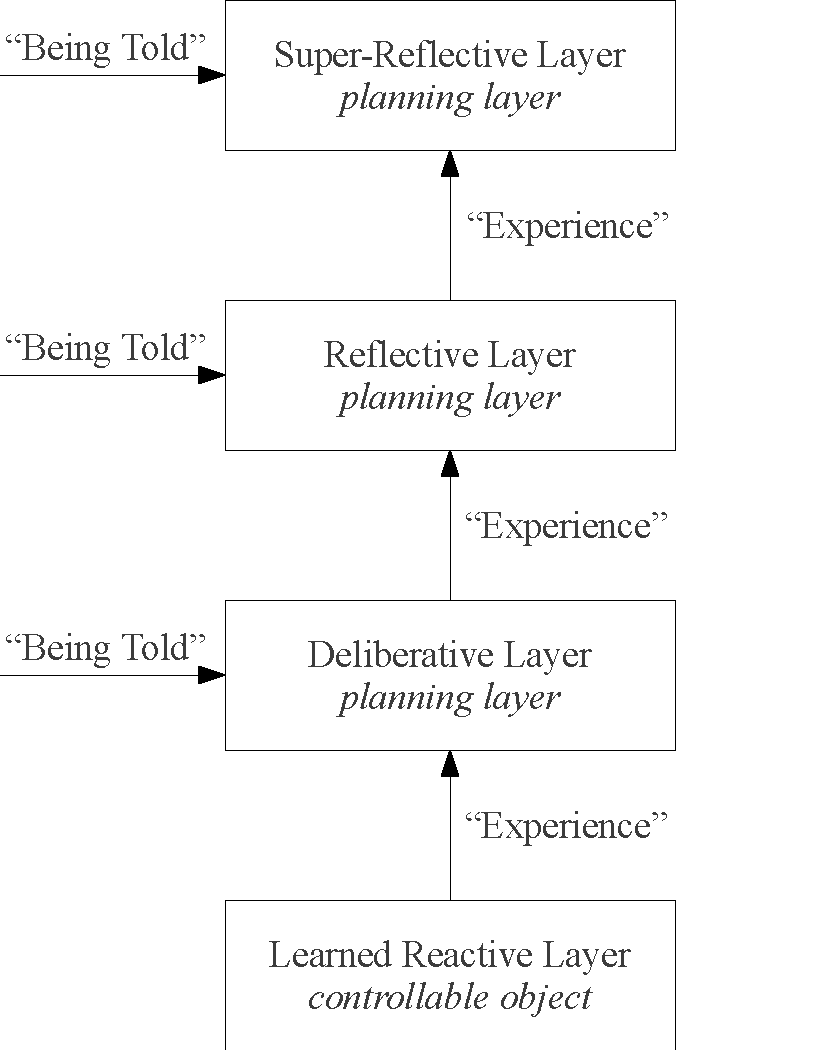
\includegraphics[width=6cm]{gfx/learning_from_being_told_in_layers}
\caption[Learning from being told and learning from experience both
  occur in each SALS planning layer.  (Reproduced from
  {\mbox{\autoref{figure:learning_from_being_told_in_layers}}})]{Learning
  from being told and learning from experience both occur in each SALS
  planning layer.  This figure is reproduced from
  {\mbox{\autoref{figure:learning_from_being_told_in_layers}}} on
  {\mbox{page~\pageref{figure:learning_from_being_told_in_layers}}} of
  the previous chapter.}
\label{figure:learning_from_being_told_in_layers_2}
\end{figure}
In this chapter, I will focus on how the SALS AI learns from the
experience of actually executing the compiled natural language plans
that result from the successful interpretation and imagination
described in the previous chapter.  Learning from experience gives the
SALS AI new hypothetical models of the effects of activating resources
in the layers below that a given planning layer is trying to control.

\section{Two Experiential Event Streams}
\label{section:two_experiential_event_streams}

Each planning layer in the SALS AI receives two event streams from the
layer below that it is trying to control: (1) a stream of all changes
in the knowledge base that the planning layer is trying to control and
(2) a stream of all activations and completions of resource
executions.  I will refer to these two asynchronous information
processing pathways as:
\begin{packed_enumerate}
\item{{\emph{partial state event reification}}, and}
\item{{\emph{resource causal rule-learning}}.}
\end{packed_enumerate}
For the deliberative planning layer, these two streams of events come
from (1) the changes in the physical knowledge base in the learned
reactive layer and (2) the activation and completion events for the
resources in the learned reactive physical agency.  Analogously, for
the reflective layer, these two streams of events come from (1)
changes in the deliberative plan knowledge base in the deliberative
layer and (2) the activation and completion events for the resources
in the deliberative plan agency.  The super-reflective layer follows
the same pattern with the two streams of events coming from (1) the
changes in the reflective plan knowledge base in the reflective layer
and (2) the activation and completion events for the resources in the
reflective plan agency.
{\mbox{\autoref{figure:deliberative_two_experiential_event_streams}}}
shows two experiential event streams that flow into the deliberative
planning layer from the learned reactive layer.
\begin{figure}
\centering
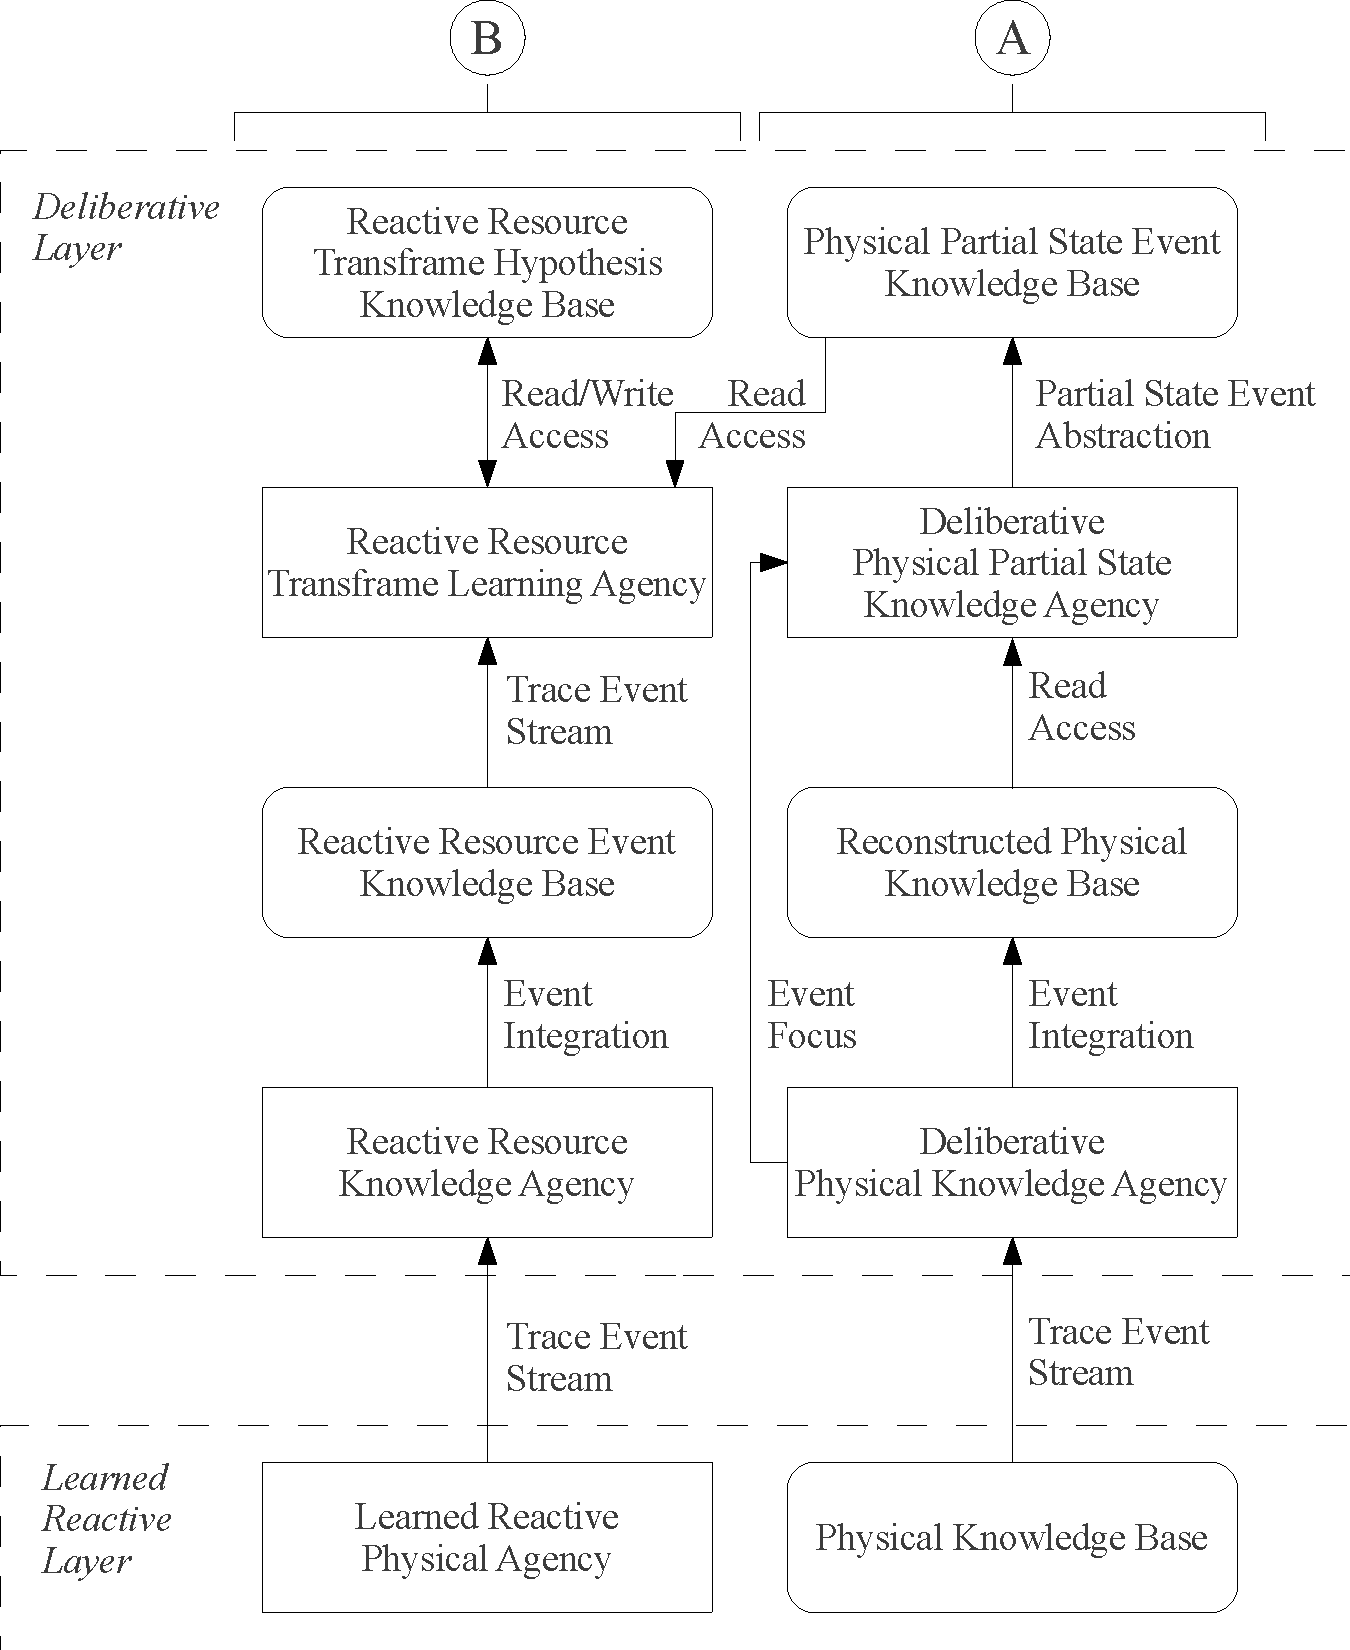
\includegraphics[width=10cm]{gfx/deliberative_two_experiential_event_streams}
\caption[Two experiential event streams flow from the learned reactive
  layer into the deliberative planning layer in the SALS AI.]{Two
  experiential event streams flow from the learned reactive layer into
  the deliberative planning layer in the SALS AI.  Analogous event
  streams flow from the deliberative planning layer to the reflective
  planning layer and from the reflective planning layer to the
  super-reflective planning layer.  Each of these two event streams
  are processed by separate information processing pathways each
  involving multiple planning layer agencies and knowledge bases
  before being woven into hypothetical models of the effects of
  resource executions of the learned reactive layer.  (A) Partial
  state event reification is performed in the first stage of
  asynchronous information processing.  Changes in the physical
  knowledge base are streamed to the deliberative planning layer where
  they are reified into the physical partial state event knowledge
  base.  (B) Resource causal rule-learning is performed in the second
  stage of asynchronous information processing.  Activation and
  completion events of resources in the learned reactive physical
  agency are streamed to the deliberative planning layer where they
  are correlated with the physical partial state event knowledge base
  where rule learning is used to develop hypothetical models of the
  effects of actions.}
\label{figure:deliberative_two_experiential_event_streams}
\end{figure}
Analogous event streams flow from the deliberative planning layer to
the reflective planning layer and from the reflective planning layer
to the super-reflective planning layer.  Each of these two event
streams are processed by separate information processing pathways each
involving multiple planning layer agencies and knowledge bases before
being woven into hypothetical models of the effects of resource
executions of the learned reactive layer.  Partial state event
reification is performed in the first stage of asynchronous
information processing.  Changes in the physical knowledge base are
streamed to the deliberative planning layer where they are reified
into the physical partial state event knowledge base.  Resource causal
rule-learning is performed in the second stage of asynchronous
information processing.  Activation and completion events of resources
in the learned reactive physical agency are streamed to the
deliberative planning layer where they are correlated with the
physical partial state event knowledge base where rule learning is
used to develop hypothetical models of the effects of actions.

{\mbox{\autoref{figure:reflective_two_experiential_event_streams}}}
shows the two experiential event streams that flow into the reflective
planning layer from the deliberative planning layer.
\begin{figure}
\centering
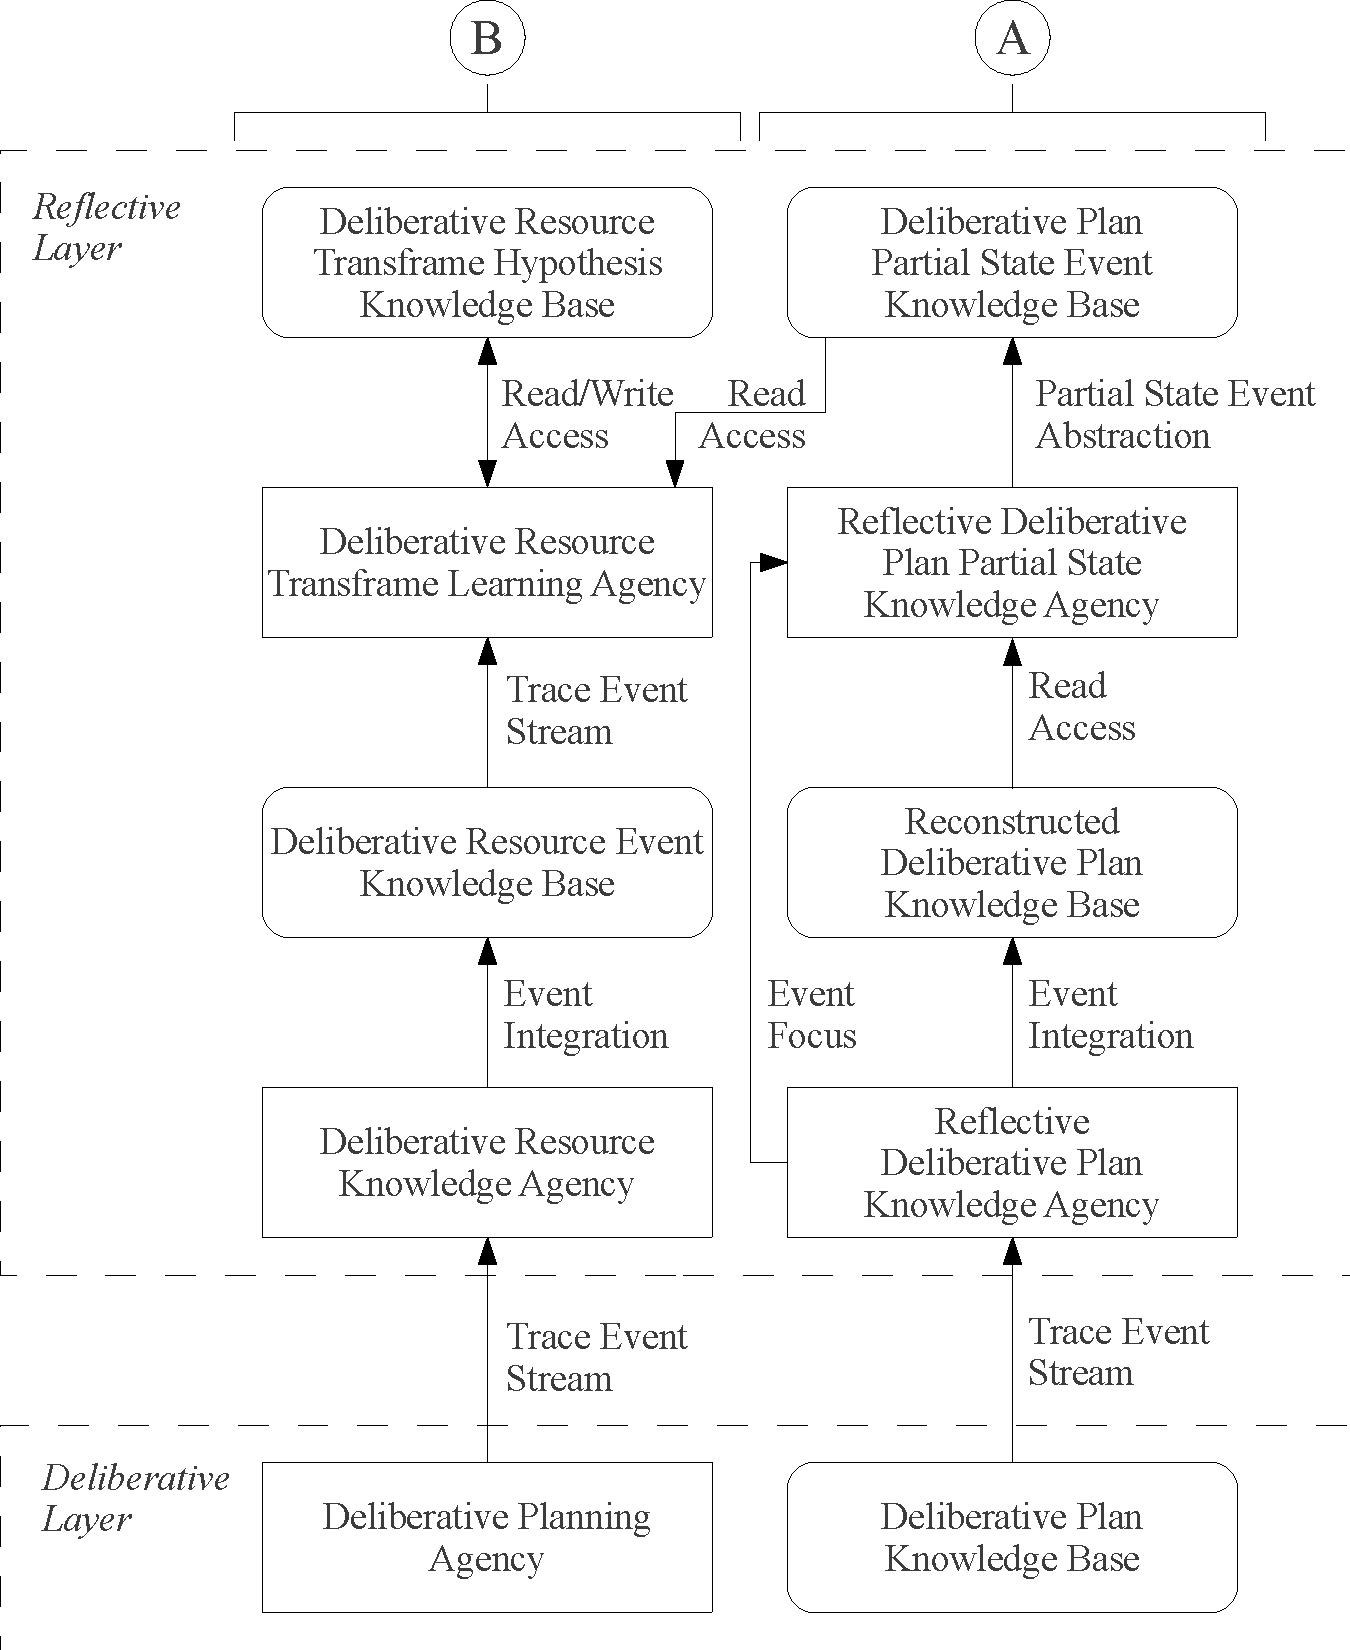
\includegraphics[width=10cm]{gfx/reflective_two_experiential_event_streams}
\caption[Two experiential event streams flow from the deliberative
  planning layer into the reflective planning layer in the SALS
  AI.]{Two experiential event streams flow from the deliberative
  planning layer into the reflective planning layer in the SALS AI.
  Analogous event streams flow from the learned reactive layer to the
  deliberative planning layer and from the reflective planning layer
  to the super-reflective planning layer.  Each of these two event
  streams are processed by separate information processing pathways
  each involving multiple planning layer agencies and knowledge bases
  before being woven into hypothetical models of the effects of
  resource executions of the deliberative planning layer.  (A) Partial
  state event reification is performed in the first stage of
  asynchronous information processing.  Changes in the deliberative
  plan knowledge base are streamed to the reflective planning layer
  where they are reified into the deliberative plan partial state
  event knowledge base.  (B) Resource causal rule-learning is
  performed in the second stage of asynchronous information
  processing.  Activation and completion events of resources in the
  deliberative planning agency are streamed to the reflective planning
  layer where they are correlated with the deliberative plan partial
  state event knowledge base where rule learning is used to develop
  hypothetical models of the effects of actions.}
\label{figure:reflective_two_experiential_event_streams}
\end{figure}
Analogous event streams flow from the learned reactive layer to the
deliberative planning layer and from the reflective planning layer to
the super-reflective planning layer.  Each of these two event streams
are processed by separate information processing pathways each
involving multiple planning layer agencies and knowledge bases before
being woven into hypothetical models of the effects of resource
executions of the deliberative planning layer.  Partial state event
reification is performed in the first stage of asynchronous
information processing.  Changes in the deliberative plan knowledge
base are streamed to the reflective planning layer where they are
reified into the deliberative plan partial state event knowledge base.
Resource causal rule-learning is performed in the second stage of
asynchronous information processing.  Activation and completion events
of resources in the deliberative planning agency are streamed to the
reflective planning layer where they are correlated with the
deliberative plan partial state event knowledge base where rule
learning is used to develop hypothetical models of the effects of
actions.

{\mbox{\autoref{figure:super_reflective_two_experiential_event_streams}}}
shows the two experiential event streams that flow into the
super-reflective planning layer from the reflective planning layer.
\begin{figure}
\centering
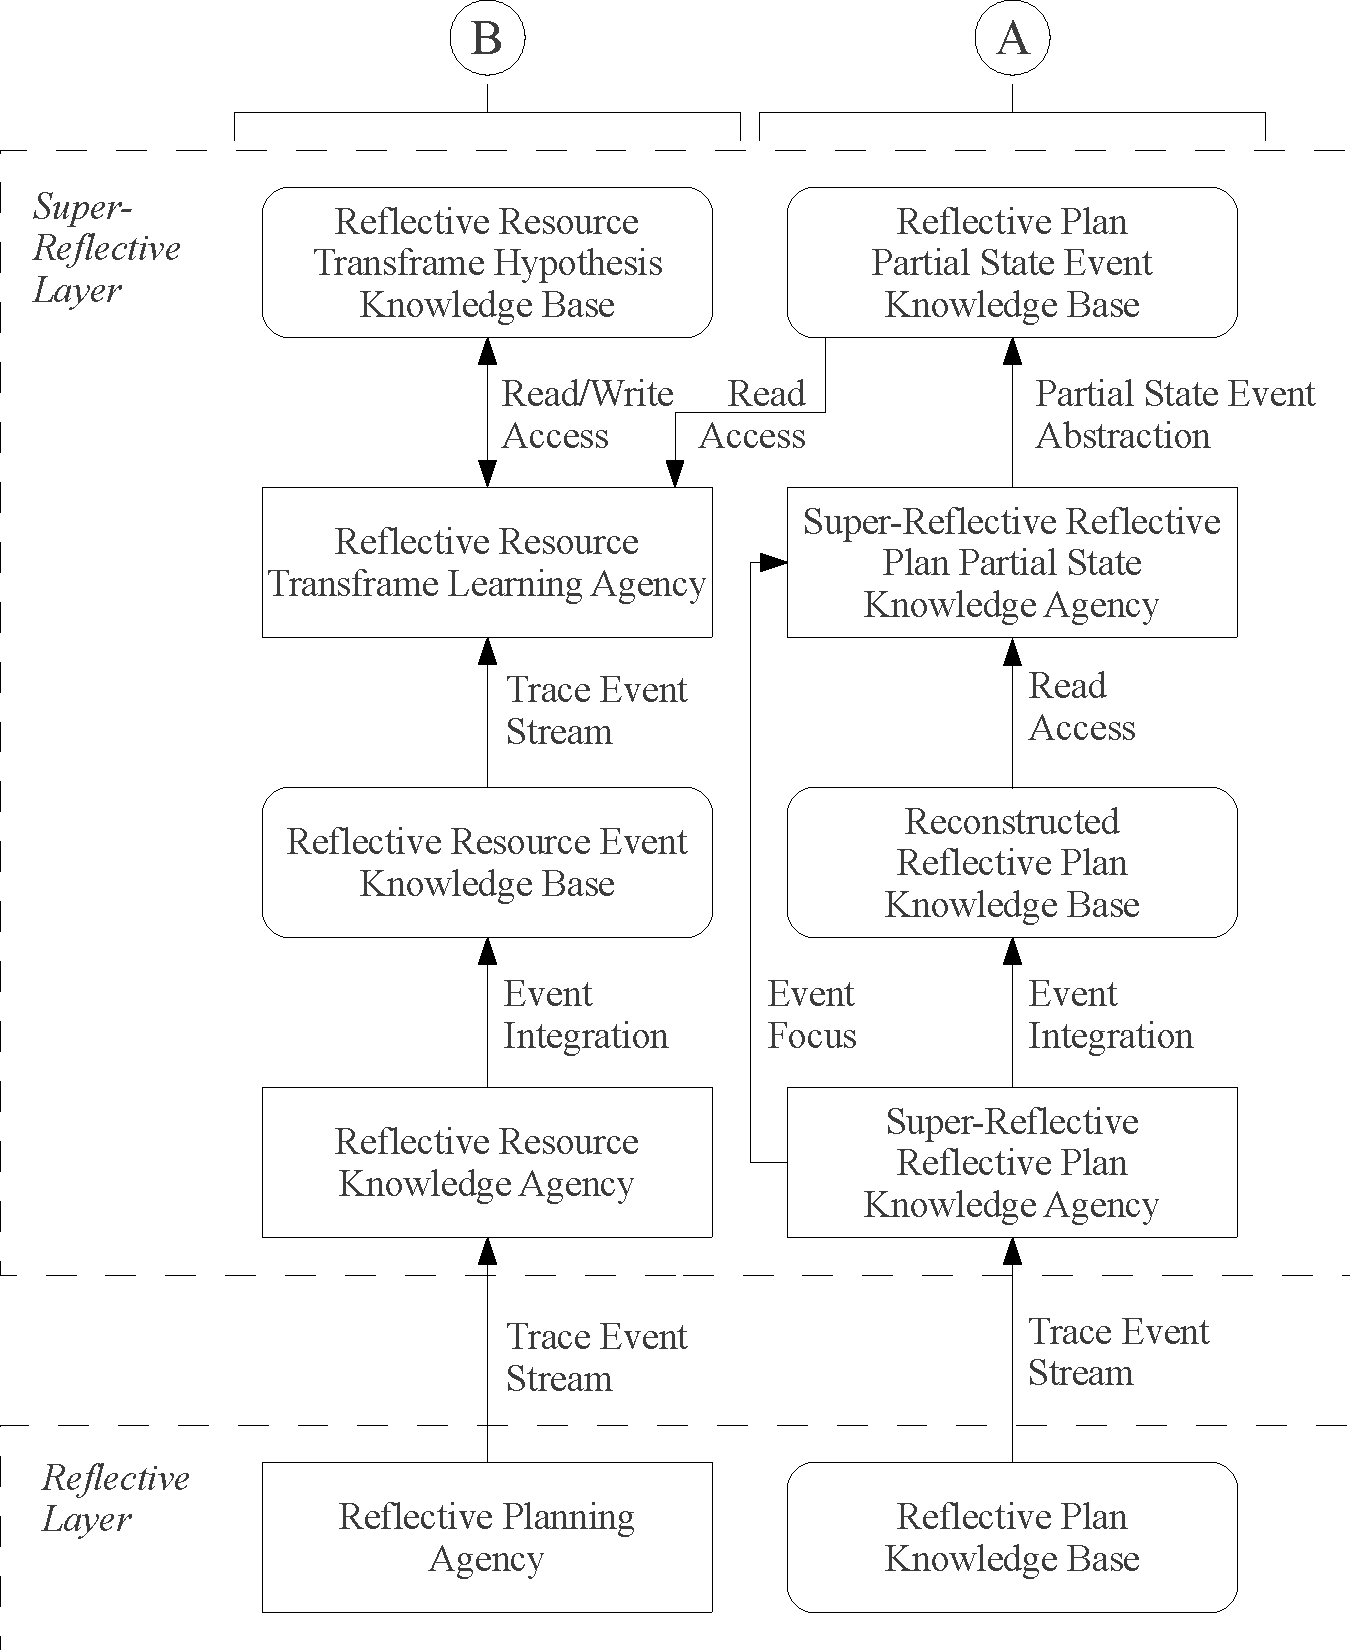
\includegraphics[width=10cm]{gfx/super_reflective_two_experiential_event_streams}
\caption[Two experiential event streams flow from the reflective
  planning layer into the super-reflective planning layer in the SALS
  AI.]{Two experiential event streams flow from the reflective
  planning layer into the super-reflective planning layer in the SALS
  AI.  Analogous event streams flow from the learned reactive layer to
  the deliberative planning layer and from the deliberative planning
  layer to the reflective planning layer.  Each of these two event
  streams are processed by separate information processing pathways
  each involving multiple planning layer agencies and knowledge bases
  before being woven into hypothetical models of the effects of
  resource executions of the reflective planning layer.  (A) Partial
  state event reification is performed in the first stage of
  asynchronous information processing.  Changes in the reflective plan
  knowledge base are streamed to the super-reflective planning layer
  where they are reified into the reflective plan partial state event
  knowledge base.  (B) Resource causal rule-learning is performed in
  the second stage of asynchronous information processing.  Activation
  and completion events of resources in the reflective planning agency
  are streamed to the super-reflective planning layer where they are
  correlated with the reflective plan partial state event knowledge
  base where rule learning is used to develop hypothetical models of
  the effects of actions.}
\label{figure:super_reflective_two_experiential_event_streams}
\end{figure}
Analogous event streams flow from the learned reactive layer to the
deliberative planning layer and from the deliberative planning layer
to the reflective planning layer.  Each of these two event streams are
processed by separate information processing pathways each involving
multiple planning layer agencies and knowledge bases before being
woven into hypothetical models of the effects of resource executions
of the reflective planning layer.  Partial state event reification is
performed in the first stage of asynchronous information processing.
Changes in the reflective plan knowledge base are streamed to the
super-reflective planning layer where they are reified into the
reflective plan partial state event knowledge base.  Resource causal
rule-learning is performed in the second stage of asynchronous
information processing.  Activation and completion events of resources
in the reflective planning agency are streamed to the super-reflective
planning layer where they are correlated with the reflective plan
partial state event knowledge base where rule learning is used to
develop hypothetical models of the effects of actions.

\section{Partial State Event Reification}
\label{section:partial_state_event_abstraction}

Partial state event reification is the first stage of asynchronous
information processing of an experiential event stream that any given
planning layer receives from the changes in the knowledge base that it
is trying to control.  {\emph{Reification}} is the process that allows
a subgraph in the layer below to be replaced by a symbol in the layer
above.  A change event object has the following six properties:
\begin{packed_enumerate}
\item{{\tt{time}}}
\item{{\tt{change-type}}}
\item{{\tt{source}}}
\item{{\tt{key-type}}}
\item{{\tt{key}}}
\item{{\tt{target}}}
\end{packed_enumerate}
The ``{\tt{time}}'' of the change event object is the clock time at
which the change occurred.  The ``{\tt{change-type}}'' property of the
change event object is one of two symbolic values: (1) ``{\tt{add}}''
or (2) ``{\tt{remove}}.''  The ``{\tt{source}}'' property of the
change event object is the frame-based object in the knowledge base
that has had a slot value added or removed.  The ``{\tt{key-type}}''
and ``{\tt{key}}'' properties of the change event object are both
symbolic values that together refer to the name of the slot of the
frame-based object in the knowledge base that has been added or
removed.  The ``{\tt{target}}'' property of the change event object is
the slot value of the frame-based object in the knowledge base that
has been added or removed.  The ``{\tt{target}}'' property can either
be a symbolic property or another frame-based object.

Every single change that occurs within the knowledge base that a
planning layer is trying to control results in a change event object
being appended to a procedurally reflective event stream that flows
into the planning layer above.  The first agency in the planning layer
that receives this event stream reconstructs a copy of the knowledge
base that it is trying to control.  Because an event stream can be
buffered, this reconstructed knowledge base can move forward in time
more slowly than the knowledge base that the planning layer is trying
to control.  Creating a reconstruction of the knowledge base under
control is important because this allows the partial state event
reification to occur asynchronously with the process that is making
changes to the knowledge base under control.  In practice, because
sets of changes to knowledge bases often occur in bursts, the
buffering of event streams usually does not lead to arbitrarily long
buffer lengths.  Once an event has been integrated into the knowledge
base reconstruction, this change results in adding or removing a
subset of partial states from the knowledge base reconstruction.  This
subset of partial state changes is computed and each change in this
subset is integrated into the partial state event knowledge base.
Computing all possible partial states would be an intractable problem,
so the SALS AI does not reify all partial states that occur in the
reconstructed knowledge base, but instead only focuses on two specific
types of partial states: (1) ``{\tt{relationship}}'' partial states
and (2) ``{\tt{property}}'' partial states.

The SALS ``{\tt{relationship}}'' and ``{\tt{property}}'' types of
partial states are the same as those described in
{\mbox{\autoref{chapter:learning_from_being_told}}} as the return
values of the ``{\tt{relationship}}'' and ``{\tt{property}}''
expressions of the SALS natural programming language.  To briefly
review, the following are the ten arguments to the
``{\tt{relationship}}'' expression, which define a SALS
``{\tt{relationship}}'' partial state:
\begin{packed_enumerate}
\item{{\tt{source-type}}}
\item{{\tt{source-key-type}}}
\item{{\tt{source-key}}}
\item{{\tt{source-value}}}
\item{{\tt{key-type}}}
\item{{\tt{key}}}
\item{{\tt{target-type}}}
\item{{\tt{target-key-type}}}
\item{{\tt{target-key}}}
\item{{\tt{target-value}}}
\end{packed_enumerate}
{\mbox{\autoref{figure:relationship_partial_state_graph_2}}} shows how
the arguments to the SALS ``{\tt{relationship}}'' partial state map to
the frame types, slot values, and properties of a frame-based
knowledge base as it is represented as a graph.
\begin{figure}
\centering
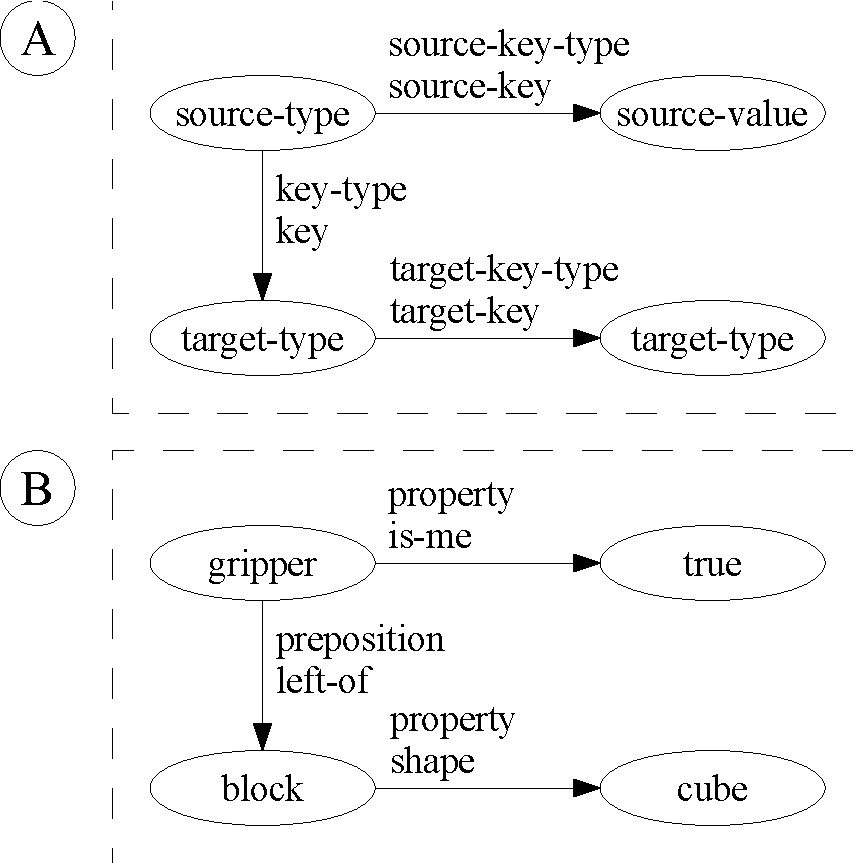
\includegraphics[width=6cm]{gfx/relationship_partial_state_graph-handdrawn}
\caption[A SALS ``{\tt{relationship}}'' partial state.  (Reproduced
  from {\mbox{\autoref{figure:relationship_partial_state_graph}}})]{A
  SALS ``{\tt{relationship}}'' partial state.  This figure is
  reproduced from
  {\mbox{\autoref{figure:relationship_partial_state_graph}}} on
  {\mbox{page~\pageref{figure:relationship_partial_state_graph}}} for
  convenience.  The (A) top graph shows the ten argument names for the
  ``{\tt{relationship}}'' expression.  The (B) bottom graph shows a
  potential partial state of the physical knowledge base that
  literally means, ``{\tt{a cube shaped block to be to the left of a
      gripper that is me}}.''}
\label{figure:relationship_partial_state_graph_2}
\end{figure}
The SALS ``{\tt{property}}'' partial state represents the conjunction
of two different properties of a frame-based object and takes the
following seven arguments:
\begin{packed_enumerate}
\item{{\tt{source-type}}}
\item{{\tt{source-key-type}}}
\item{{\tt{source-key}}}
\item{{\tt{source-value}}}
\item{{\tt{key-type}}}
\item{{\tt{key}}}
\item{{\tt{value}}}
\end{packed_enumerate}
{\mbox{\autoref{figure:relationship_partial_state_graph_2}}} shows how
the arguments to the ``{\tt{property}}'' expression map to the frame
types, slot values, and properties of a frame-based knowledge base
that is represented as a graph.
\begin{figure}
\centering
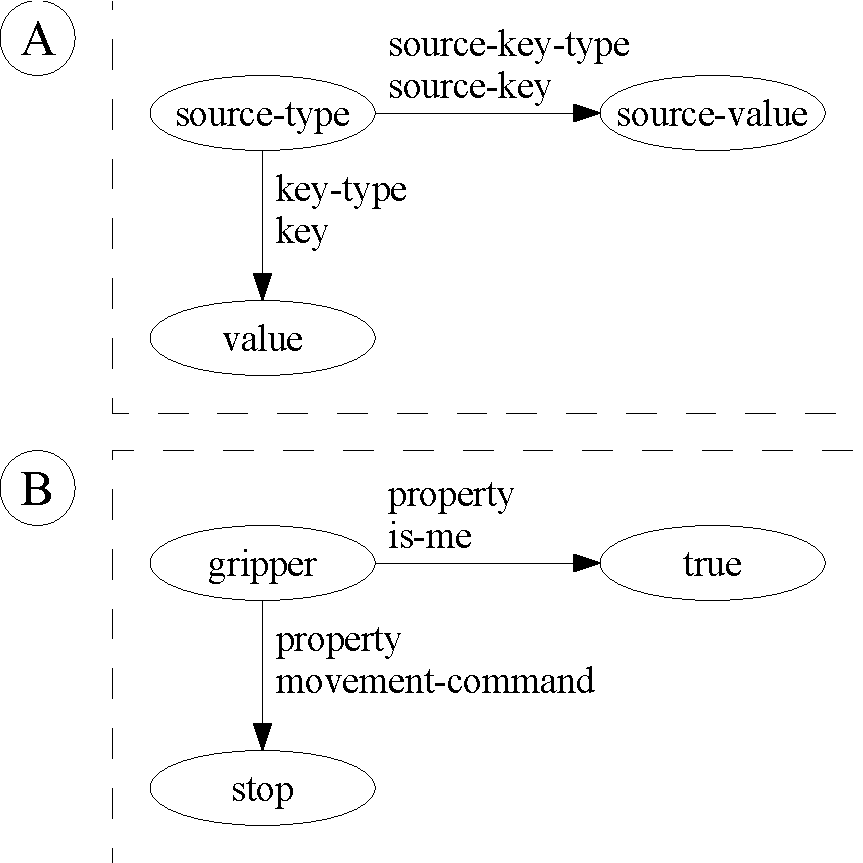
\includegraphics[width=6cm]{gfx/property_partial_state_graph-handdrawn}
\caption[The SALS ``{\tt{property}}'' partial state object.
  (Reproduced from
  {\mbox{\autoref{figure:property_partial_state_graph}}})]{The SALS
  ``{\tt{property}}'' partial state object.  This figure is reproduced
  from {\mbox{\autoref{figure:property_partial_state_graph}}} on
  {\mbox{page~\pageref{figure:property_partial_state_graph}}} for
  convenience.  The (A) top graph shows the seven argument names for
  the ``{\tt{property}}'' expression.  The (B) bottom graph shows a
  potential partial state of the physical knowledge base that
  literally means, ``{\tt{a gripper to be me and have a stop movement
      command}}.''}
\label{figure:property_partial_state_graph_2}
\end{figure}
While the reception of a single ``{\tt{add}}'' or ``{\tt{remove}}''
change event object only adds or removes a single edge from the
knowledge base, this results in potentially adding or removing many
``{\tt{relationship}}'' and ``{\tt{property}}'' type partial states to
or from that knowledge base.
{\mbox{\autoref{figure:relationship_partial_state_abstraction_remove}}}
shows how a ``{\tt{remove}}'' change event object is integrated into
the reconstructed physical knowledge base.
\begin{figure}
\centering
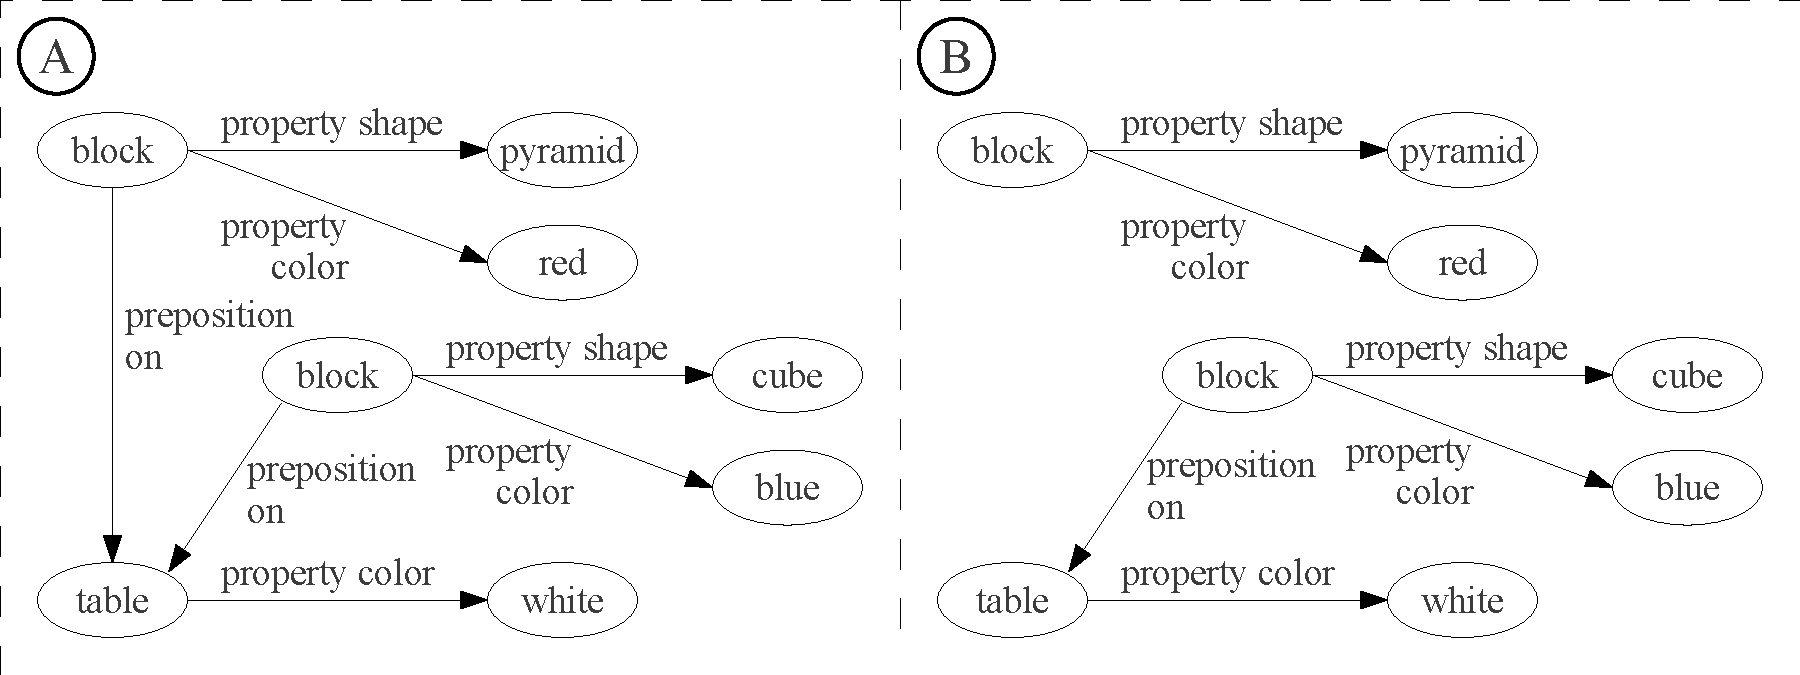
\includegraphics[width=12cm]{gfx/relationship_partial_state_abstraction_remove}
\caption[A ``{\tt{remove}}'' change event object is integrated into
  the reconstructed physical knowledge base.]{A ``{\tt{remove}}''
  change event object is integrated into the reconstructed physical
  knowledge base.  In this case, a pyramid shaped block is no longer
  related by the ``{\tt{on}}'' relationship to a white colored table
  object.  While the reception of a single ``{\tt{remove}}'' change
  event object only removes a single edge from the knowledge base,
  this results in potentially removing many partial states from that
  knowledge base.  (A) The reconstructed physical knowledge base in
  the deliberative layer \emph{before} a ``{\tt{remove}}'' change
  event object is received by the deliberative physical knowledge
  agency.  (B) The reconstructed physical knowledge base in the
  deliberative layer \emph{after} a ``{\tt{remove}}'' change event
  object is received by the deliberative physical knowledge agency.}
\label{figure:relationship_partial_state_abstraction_remove}
\end{figure}
{\mbox{\autoref{figure:relationship_partial_state_abstraction_add}}}
shows how an ``{\tt{add}}'' change event object is integrated into the
reconstructed physical knowledge base.
\begin{figure}
\centering
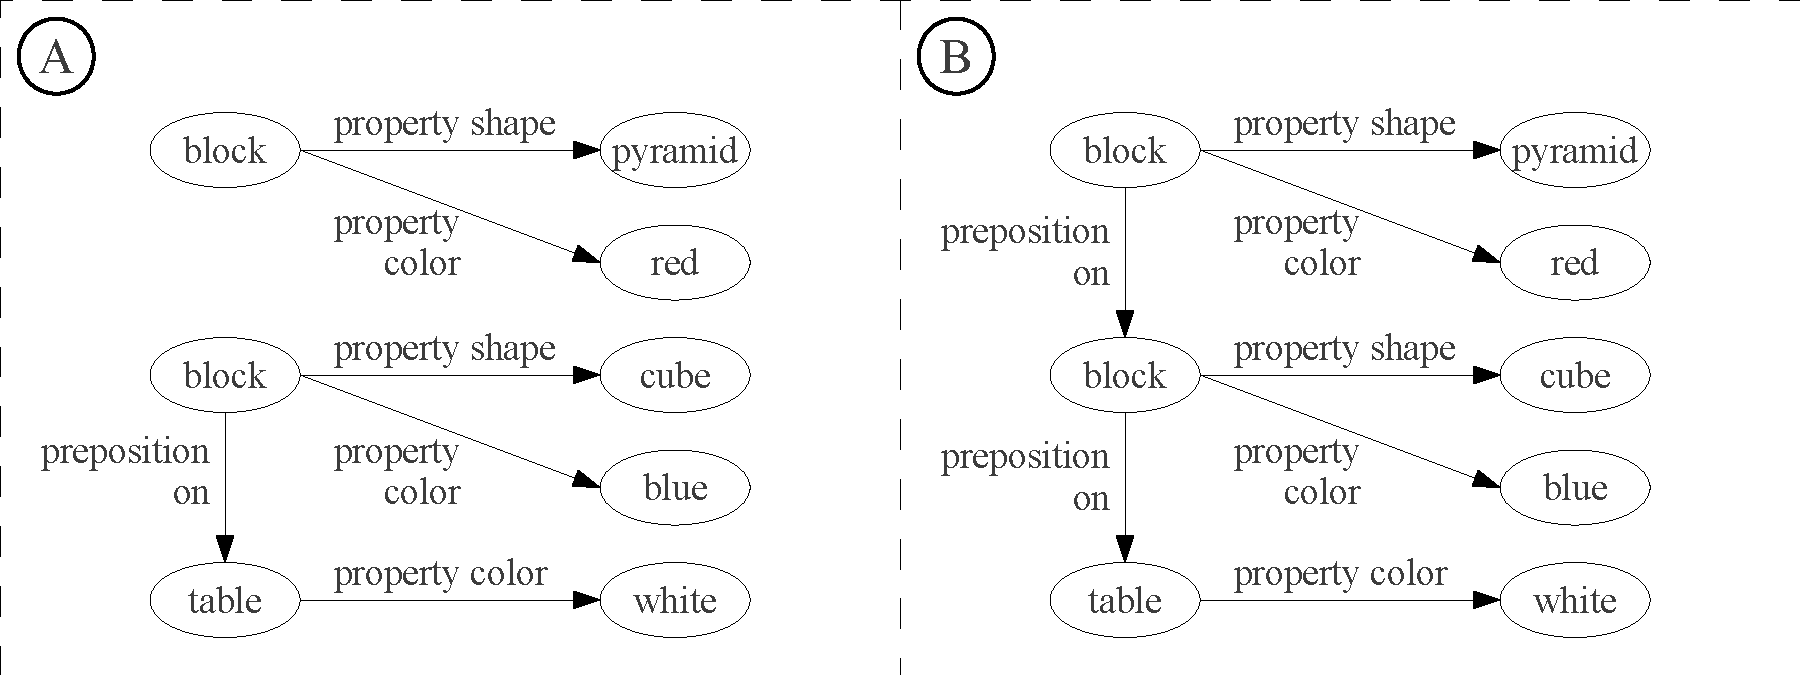
\includegraphics[width=12cm]{gfx/relationship_partial_state_abstraction_add}
\caption[An ``{\tt{add}}'' change event object is integrated into the
  reconstructed physical knowledge base.]{An ``{\tt{add}}'' change
  event object is integrated into the reconstructed physical knowledge
  base.  In this case, a pyramid shaped block is now related by the
  ``{\tt{on}}'' relationship to a cube shaped block object.  While the
  reception of a single ``{\tt{add}}'' change event object only adds a
  single edge to the knowledge base, this results in potentially
  adding many partial states to that knowledge base.  (A) The
  reconstructed physical knowledge base in the deliberative layer
  \emph{before} an ``{\tt{add}}'' change event object is received by
  the deliberative physical knowledge agency.  (B) The reconstructed
  physical knowledge base in the deliberative layer \emph{after} an
  ``{\tt{add}}'' change event object is received by the deliberative
  physical knowledge agency.}
\label{figure:relationship_partial_state_abstraction_add}
\end{figure}

The fact that the SALS cognitive architecture only has two types of
partial state objects, the ``{\tt{relationship}}'' and
``{\tt{property}}'' partial state objects, is a current limitation of
the SALS cognitive architecture.  This means that the architecture
cannot pursue goals or make judgments about other potentially more
complex types of partial states in the knowledge bases that planning
layers are attempting to control.  For example, the
``{\tt{property}}'' partial state object is only able to describe
partial states of a knowledge base that involve two properties of a
single frame-based object, while the ``{\tt{relationship}}'' partial
state object is only able to describe partial states of a knowledge
base that involve one relationship between two frame-based objects
with one symbolic property each.  While these two types of partial
state objects can sometimes be combined in clever ways to describe
some more complex partial states, generally, if a goal condition
requires a partial state object description of three or more
frame-based objects that are related with three or more properties
each, there are not currently SALS partial state objects that directly
describe these more complex types of partial states.  In
{\mbox{\autoref{chapter:future}}}, I will describe an idea for how
types of partial states in the SALS cognitive architecture could be
reified in future research to include any specific type of subgraph in
a frame-based knowledge base, but for now, the reification of the
``{\tt{relationship}}'' and ``{\tt{property}}'' types in SALS are each
specially implemented to efficiently reify each of these types of
partial state objects from a frame-based knowledge base, avoiding the
NP-complete subgraph isomorphism decision problem
\cite[]{messmer:1995,messmer:2000} implied by a careless
implementation of this more specific problem, which gains in
efficiency by taking advantage of specially implemented locally
directed searches for each different type of partial state object.
After a change event from the physical knowledge base is received by
the deliberative physical knowledge agency, the same change event is
passed to the deliberative physical partial state agency to focus a
local search around this change in the reconstructed physical
knowledge base that searches for ``{\tt{property}}'' and
``{\tt{relationship}}'' partial state objects.  If the change event
object is a ``{\tt{remove}}'' event object, the local search in the
reconstructed physical knowledge base is performed \emph{before} the
reconstructed physical knowledge base is updated, while if the change
event object is an ``{\tt{add}}'' event object, the local search in
the reconstructed physical knowledge base is performed \emph{after}
the reconstructed physical knowledge base is updated.

When a partial state object is found to be added by the deliberative
physical partial state agency, a {\emph{partial state event}} object
is added to the physical partial state event knowledge base in the
deliberative layer.  A partial state event object consists of the
following three properties:
\begin{packed_enumerate}
\item{{\tt{start-time}}}
\item{{\tt{end-time}}}
\item{{\tt{partial-state}}}
\end{packed_enumerate}
A partial state event object that has just been created has an
absolute ``{\tt{start-time}}'' value, which is a copy of the
``{\tt{time}}'' slot value of the change event object from the
physical knowledge base in the learned reactive layer.  The
``{\tt{end-time}}'' value for the partial state event object is
initially unknown, so the symbol ``{\tt{after}}'' is used to indicate
that the partial state event object has not yet ended.  The
``{\tt{partial-state}}'' slot of the partial state event object is a
reference to the partial state object that has been found in the
reconstructed physical knowledge base in the deliberative layer.  When
a partial state object is found to be removed by the deliberative
physical partial state agency, an absolute ``{\tt{end-time}}'' slot
value is added to the partial state event object that was previously
added to the physical partial state event knowledge base.

Although I have described this process of partial state event
reification in terms of the deliberative layer reifying partial state
event objects from a stream of change event objects derived from
changes in the physical knowledge base in the learned reactive layer,
an analogous process exists between each planning layer and the
knowledge base in the layer below that it is trying to control.  The
reflective deliberative plan knowledge agency receives a stream of
change event objects from the deliberative plan knowledge base in the
deliberative layer, and the reflective deliberative plan partial state
knowledge agency in the reflective layer reifies the partial states in
the reconstructed deliberative plan knowledge base into partial state
event objects that are added to the deliberative plan partial state
event knowledge base in the reflective layer.  Similarly, the
super-reflective layer reifies partial states of the reflective plan
knowledge base and adds new partial state event objects to the
reflective plan partial state event knowledge base.

\section{Resource Causal Rule-Learning}
\label{section:resource_execution_event_causal_rule_learning}

The second asynchronous stage of information processing involved in
asynchronously learning from experience in the SALS AI is the
{\emph{resource causal rule-learning}} stage.  I will first focus on
how this stage works when the deliberative layer receives a stream of
procedurally reflective events from the learned reactive layer with
the understanding that an analogous asynchronous information process
exists in each planning layer in the SALS AI.  The reactive resource
knowledge agency in the deliberative layer receives a stream of
activation and completion event objects from the resources in the
learned reactive physical agency of the learned reactive layer.  When
an activation event object is received by the reactive resource
knowledge agency in the deliberative layer, a {\emph{resource
    execution event}} object is added to the reactive resource event
knowledge base.  Like the partial state event object, a resource
execution event object consists of the following three properties:
\begin{packed_enumerate}
\item{{\tt{start-time}}}
\item{{\tt{end-time}}}
\item{{\tt{resource}}}
\end{packed_enumerate}
When a new resource execution event object is created, its
``{\tt{start-time}}'' slot value is copied from the ``{\tt{time}}''
slot of the activation event object that the reactive resource
knowledge agency in the deliberative layer has received from the
learned reactive physical agency in the learned reactive layer.  When
a completion event object is received from the learned reactive layer,
the ``{\tt{end-time}}'' slot value of the appropriate resource
execution event object is copied from the ``{\tt{time}}'' slot of the
completion event object.  Transframes \cite[]{minsky:1975} represent
change.  When a resource execution event has completed, a transframe
is created that keeps track of the added or removed information in
the physical partial state event knowledge base between the
``{\tt{start-time}}'' and ``{\tt{end-time}}'' slot values of the
resource execution event.  Creating this transframe requires
retrieving all of the partial state events that intersect with the
``{\tt{start-time}}'' slot value as well as all of the partial state
events that intersect with the ``{\tt{end-time}}'' slot value.

Every knowledge base that contains event objects in the SALS AI is
organized for indexing by time by using an interval tree that stores
all events that have been added to that knowledge base.  These types
of knowledge bases in the SALS AI are called {\emph{event knowledge
    bases}}, and they have a $O(\log{(n)})$ time complexity for
retrieving events by time, given that $n$ is the number of events in
the event knowledge base.  To maintain consistency within the interval
tree within the event knowledge base, some precautions must be taken
when changing the values of the ``{\tt{start-time}}'' and
``{\tt{end-time}}'' slots of any event object, which could potentially
invalidate the entire interval tree.  To make this bookkeeping
transparent to the plan execution, reflectively traced callbacks are
called whenever a slot value is added to or removed from the event
knowledge base.  If the slot value refers to the ``{\tt{start-time}}''
or the ``{\tt{end-time}}'' of an event object, the event object is
first removed from the interval tree with its old slot value, the slot
value is changed, then the event object is inserted into the interval
tree once the slot value change is complete.  This means that the plan
simply executes normally, which reflectively causes the addition and
removal of event objects to the reconstructed event knowledge base,
freely changing their ``{\tt{start-time}}'' and ``{\tt{end-time}}''
slot values as callbacks take care of the interval tree organization.

\section{Deliberatively Learning about Physical Actions}

\begin{table}
\centering
\begin{tabular}{p{0.5cm}p{7cm}}
A. & \begin{tabular}{|p{7cm}|}
       \hline
       ``{\tt{a pyramid shaped block to be sitting on a white colored table}}'' \\
       \hline
     \end{tabular} \\
B. & \begin{tabular}{|p{7cm}|}
       \hline
       ``{\tt{a gripper that is me to be above a pyramid shaped block}}'' \\
       \hline
     \end{tabular} \\
C. & \begin{tabular}{|p{7cm}|}
       \hline
       ``{\tt{a gripper that is me to be holding a cube shaped block}}'' \\
       \hline
     \end{tabular} \\
D. & \begin{tabular}{|p{7cm}|}
       \hline
       ``{\tt{a cube shaped block to be sitting on a pyramid shaped block}}'' \\
       \hline
     \end{tabular} \\
E. & \begin{tabular}{|p{7cm}|}
       \hline
       ``{\tt{a cube shaped block to be sitting on a white colored table}}'' \\
       \hline
     \end{tabular} \\
\end{tabular}
\caption[A selection of physical partial states that occur during the
  example learning story presented in
  {\mbox{\autoref{chapter:introduction}}}.]{A selection of physical
  partial states that occur during the example learning story
  presented in {\mbox{\autoref{chapter:introduction}}}.}
\label{table:example_physical_partial_states_during_learning}
\end{table}
\begin{table}
\centering
\begin{tabular}{p{1cm}|p{1.5cm}|p{1.5cm}p{1.5cm}|p{1.5cm}p{1.5cm}|}
{\emph{Partial State}} &{\emph{Precond.}} &{\emph{Expected Trans.}}  &{\emph{Expected Postcond.}}  &{\emph{Actual Trans.}}  &{\emph{Actual Postcond.}}  \\
\hline
A                      & $1$            &                       & $1$                   &                       & $1$                   \\
B                      & $1$            &                       & $1$                   &                       & $1$                   \\
C                      & $1$            & $-$                   & $0$                   & $-$                   & $0$                   \\
D                      & $0$            & \cellcolor{red!10}$+$ & \cellcolor{red!10}$1$ & \cellcolor{red!10}    & \cellcolor{red!10}$0$ \\
E                      & $0$            & \cellcolor{red!10}    & \cellcolor{red!10}$0$ & \cellcolor{red!10}$+$ & \cellcolor{red!10}$1$ \\
\hline
\end{tabular}
\caption[An example expectation failure when the deliberative layer
  incorrectly hypothesizes physical partial states.]{An example
  expectation failure when the deliberative layer incorrectly
  hypothesizes physical partial states.  Refer to
  {\mbox{\autoref{table:example_physical_partial_states_during_learning}}}
  for definitions of partial states, A--E.  Shown are the imagined and
  actual transitions for executing the action of dropping a cube on a
  pyramid.  The fact that the expected transframe does not match the
  actual transframe presents the AI with a learning opportunity.  The
  shaded area highlights the expectation failure.  The symbol ``$1$''
  represents that the partial state exists.  The symbol ``$0$''
  represents that the partial state does not exist.  The symbol
  ``$+$'' represents that the partial state is added.  The symbol
  ``$-$'' represents that the partial state is removed.}
\label{table:example_physical_expectation_failure}
\end{table}
{\mbox{\autoref{table:example_physical_partial_states_during_learning}}}
and {\mbox{\autoref{table:example_physical_expectation_failure}}}
present an example of a learning opportunity in the deliberative layer
because of a failure to predict the effects of physical actions during
deliberative planning.  This learning opportunity results from an
expectation failure that occurs when the SALS AI imagines and then
actually executes the action of dropping a cube on a pyramid.  Once
the partial state transframe has been computed for a given action
resource execution event, this transframe is used to train a
rule-learning algorithm that attempts to categorize the partial state
preconditions for different sets of the possible ``{\tt{add}}'' ($+$)
and ``{\tt{remove}}'' ($-$) changes.  A rule-learning algorithm is
used in the SALS AI to predict the transframe that will result from
executing a resource in given preconditions.  This rule-learning
algorithm is based on {\emph{version spaces}} \cite[]{mitchell:1997}.

Version spaces are an efficient representation for all possible
conjunctive functions that map a set of binary inputs to a single
binary output.  These functions are also called {\emph{hypotheses}}.
When these hypotheses turn out to be wrong given new data, the
hypothesis version space is refined.  In the case of a false positive,
the most general functions of the version space are specialized.  In
the case of a false negative, the most specific hypotheses of the
version space are generalized.
\begin{table}
\centering
\begin{tabular}{p{1cm}|p{1.5cm}|p{1.5cm}|}
{\emph{change}}        & {\emph{positive example}}      & {\emph{negative example}}      \\
                       & {\tt{ABCDE}}                   & {\tt{ABCDE}}                   \\
\hline
$-$A                   &                                & {\tt{11100}}                   \\
$+$A                   &                                & {\tt{11100}}                   \\
$-$B                   &                                & {\tt{11100}}                   \\
$+$B                   &                                & {\tt{11100}}                   \\
$-$C                   & {\tt{11100}}                   &                                \\
$+$C                   &                                & {\tt{11100}}                   \\
$-$D                   &                                & {\tt{11100}}                   \\
\cellcolor{red!10}$+$D & \cellcolor{red!10}             & \cellcolor{red!10}{\tt{11100}} \\
$-$E                   &                                & {\tt{11100}}                   \\
\cellcolor{red!10}$+$E & \cellcolor{red!10}{\tt{11100}} & \cellcolor{red!10}             \\
\hline
\end{tabular}
\caption[Positive and negative training preconditions from the
  physical learning example presented previously in
  {\mbox{\autoref{table:example_physical_expectation_failure}}}.]{Positive
  and negative training preconditions from the physical learning
  example presented previously in
  {\mbox{\autoref{table:example_physical_expectation_failure}}}.  This
  learning situation involves two changes that led to incorrect
  predictions: ``$+$D'' and ``$+$E.''  The addition of partial state
  ``D'' is incorrectly expected, while the addition of partial state
  ``E'' is incorrectly {\emph{not}} expected.  The shaded areas
  represent the expectation failure, the failure to predict the
  correct state changes.  The precondition state, ``{\tt{11100}},''
  can be used as a positive or negative training example for the
  appropriate version hypothesis spaces for learning new rules for
  predicting these changes correctly in the future.}
\label{table:example_physical_transframe_rule_learning}
\end{table}
{\mbox{\autoref{table:example_physical_transframe_rule_learning}}}
shows an example of preconditions being used as positive and negative
training examples for the version hypothesis spaces that lead to an
expectation failure in the example previously presented in
{\mbox{\autoref{table:example_physical_expectation_failure}}}.  In the
SALS AI, the binary inputs to the rule-learning algorithm represent
whether or not a partial state exists in the preconditions of the
resource execution event.  The single binary output from the
rule-learning algorithm represents whether or not a set of partial
state transframe changes will be the result of executing the resource
in the given partial state preconditions.  These hypothesis version
spaces are used to predict the effects of natural language plans in
the counterfactual knowledge base of each planning layer during the
interpretation and imagination process described in
{\mbox{\autoref{chapter:learning_from_being_told}}}.

\section{Reflectively Learning about Deliberative Actions}

\begin{table}
\centering
\begin{tabular}{p{0.5cm}p{7cm}}
A. & \begin{tabular}{|p{7cm}|}
       \hline
       ``{\tt{a deliberative planner to be focusing on a plan that has been imagined}}'' \\
       \hline
     \end{tabular} \\
B. & \begin{tabular}{|p{7cm}|}
       \hline
       ``{\tt{a deliberative planner to be focused on a plan that is hypothesized to cause a cube to be on a pyramid}}'' \\
       \hline
     \end{tabular} \\
C. & \begin{tabular}{|p{7cm}|}
       \hline
       ``{\tt{a deliberative planner to be focused on a plan that is hypothesized to cause a pyramid to be on a cube}}'' \\
       \hline
     \end{tabular} \\
D. & \begin{tabular}{|p{7cm}|}
       \hline
       ``{\tt{a deliberative planner to be focusing on a plan that has been executed}}'' \\
       \hline
     \end{tabular} \\
E. & \begin{tabular}{|p{7cm}|}
       \hline
       ``{\tt{a deliberative planner to be focused on a plan that has failed in execution}}'' \\
       \hline
     \end{tabular} \\
\end{tabular}
\caption[A selection of deliberative plan partial states that occur
  during the example learning story presented in
  {\mbox{\autoref{chapter:introduction}}}.]{A selection of
  deliberative plan partial states that occur during the example
  learning story presented in
  {\mbox{\autoref{chapter:introduction}}}.}
\label{table:example_deliberative_plan_partial_states_during_learning}
\end{table}
\begin{table}
\centering
\begin{tabular}{p{1cm}|p{1.5cm}|p{1.5cm}p{1.5cm}|p{1.5cm}p{1.5cm}|}
{\emph{Partial State}} &{\emph{Precond.}} &{\emph{Expected Trans.}} &{\emph{Expected Postcond.}} &{\emph{Actual Trans.}} &{\emph{Actual Postcond.}} \\
\hline
A                      & $1$              &                         & $1$                        &                       & $1$                      \\
B                      & $1$              &                         & $1$                        &                       & $1$                      \\
C                      & $0$              &                         & $0$                        &                       & $0$                      \\
D                      & $0$              & $+$                     & $1$                        & $+$                   & $1$                      \\
E                      & $0$              & \cellcolor{red!10}      & \cellcolor{red!10}$0$      & \cellcolor{red!10}$+$ & \cellcolor{red!10}$1$    \\
\hline
\end{tabular}
\caption[An example expectation failure when the reflective layer
  incorrectly hypothesizes deliberative plan partial states.]{An
  example expectation failure when the reflective layer incorrectly
  hypothesizes deliberative plan partial states.  Refer to
  {\mbox{\autoref{table:example_deliberative_plan_partial_states_during_learning}}}
  for definitions of partial states, A--E.  Shown are the imagined and
  actual transitions for executing the action of executing a plan to
  ``{\tt{stack a cube on a pyramid}}.''  The fact that the expected
  transframe does not match the actual transframe presents the AI with
  a learning opportunity.  The shaded area highlights the expectation
  failure.  The symbol ``$1$'' represents that the partial state
  exists.  The symbol ``$0$'' represents that the partial state does
  not exist.  The symbol ``$+$'' represents that the partial state is
  added.  The symbol ``$-$'' represents that the partial state is
  removed.}
\label{table:example_deliberative_plan_expectation_failure}
\end{table}
{\mbox{\autoref{table:example_deliberative_plan_partial_states_during_learning}}}
and
{\mbox{\autoref{table:example_deliberative_plan_expectation_failure}}}
present an example of a learning opportunity in the reflective layer
because of a failure to predict the effects of deliberative planning
actions during reflective planning.  This learning opportunity results
from an expectation failure that occurs when the SALS AI imagines and
then actually executes the action of executing a plan to ``{\tt{stack
    a cube on a pyramid}}.''  In the example story presented in
{\mbox{\autoref{chapter:introduction}}}, the reflective layer predicts
that executing the plan to ``{\tt{stack a cube on a pyramid}}'' will
not result in any deliberative plans having physical execution
failures, a negative goal state that the reflective planner is trying
to avoid in the deliberative plan knowledge base.  When the reflective
plan decides to execute this deliberative plan, based on the
prediction that it will not lead to failure, there is an expectation
failure at the reflective layer when the deliberative plan actually
does fail during its execution.  This expectation failure in the
reflective layer is shown as highlighted areas of
{\mbox{\autoref{table:example_deliberative_plan_partial_states_during_learning}}}
and
{\mbox{\autoref{table:example_deliberative_plan_expectation_failure}}}.
This failure of the reflective layer to predict the effects of
deliberative actions on the deliberative plan knowledge base presents
the SALS AI with a learning opportunity at the reflective layer.
\begin{table}
\centering
\begin{tabular}{p{1cm}|p{1.5cm}|p{1.5cm}|}
{\emph{change}}        & {\emph{positive example}}      & {\emph{negative example}}      \\
                       & {\tt{ABCDE}}                   & {\tt{ABCDE}}                   \\
\hline
$-$A                   &                                & {\tt{11000}}                   \\
$+$A                   &                                & {\tt{11000}}                   \\
$-$B                   &                                & {\tt{11000}}                   \\
$+$B                   &                                & {\tt{11000}}                   \\
$-$C                   &                                & {\tt{11000}}                   \\
$+$C                   &                                & {\tt{11000}}                   \\
$-$D                   &                                & {\tt{11000}}                   \\
$+$D                   & {\tt{11000}}                   &                                \\
$-$E                   &                                & {\tt{11000}}                   \\
\cellcolor{red!10}$+$E & \cellcolor{red!10}{\tt{11000}} & \cellcolor{red!10}             \\
\hline
\end{tabular}
\caption[Positive and negative training preconditions from the
  deliberative plan learning example presented previously in
  {\mbox{\autoref{table:example_physical_expectation_failure}}}.]{Positive
  and negative training preconditions from the deliberative plan
  learning example presented previously in
  {\mbox{\autoref{table:example_deliberative_plan_expectation_failure}}}.
  This learning situation involves one change that led to an incorrect
  prediction: ``$+$E.''  The addition of partial state ``E'' is
  incorrectly {\emph{not}} expected.  The shaded areas represent the
  expectation failure, the failure to predict the correct state
  changes.  The precondition state, ``{\tt{11000}},'' can be used as a
  positive training example for the appropriate version hypothesis
  spaces for learning new rules for predicting this change correctly
  in the future.}
\label{table:example_deliberative_plan_transframe_rule_learning}
\end{table}
{\mbox{\autoref{table:example_deliberative_plan_transframe_rule_learning}}}
shows an example of preconditions being used as positive and negative
training examples for the version hypothesis spaces that lead to an
expectation failure in the example previously presented in
{\mbox{\autoref{table:example_physical_expectation_failure}}}.

\section{Lazy Allocation of Hypothesis Spaces}

It would be inefficient to allocate a new hypothesis version space
object for each type of ``{\tt{add}}'' or ``{\tt{remove}}'' change in
a partial state transframe for a given action resource because sets of
partial state changes often occur together and multiple hypothesis
version space rule-learning algorithms would contain redundant
information for these sets of partial state changes.  To reduce the
number of hypothesis version spaces that are allocated to each action
resource to predict the partial state changes that it may cause when
executed, each co-occurring set of partial state changes for each
action resource is calculated.

For example, consider the physical partial state changes presented in
{\mbox{\autoref{table:example_physical_transframe_rule_learning}}}.
For the moment, imagine that the AI has had no previous experience and
that the information in this table is the only experience available to
the deliberative layer's hypothesis version space rule-learning
algorithm.  In this case, notice that many of the partial state
changes have exactly the same positive and negative training examples
thus far.
\begin{table}
\centering
\begin{tabular}{p{2cm}|p{1cm}|p{1.5cm}|p{1.5cm}|}
hypothesis version space change set & {\emph{change}}        & {\emph{positive example}}      & {\emph{negative example}}      \\
                                    &                        & {\tt{ABCDE}}                   & {\tt{ABCDE}}                   \\
\hline
\#1                                 & $-$A                   &                                & {\tt{11100}}                   \\
                                    & $+$A                   &                                & {\tt{11100}}                   \\
                                    & $-$B                   &                                & {\tt{11100}}                   \\
                                    & $+$B                   &                                & {\tt{11100}}                   \\
                                    & $+$C                   &                                & {\tt{11100}}                   \\
                                    & $-$D                   &                                & {\tt{11100}}                   \\
                                    & $+$D                   &                                & {\tt{11100}}                   \\
                                    & $-$E                   &                                & {\tt{11100}}                   \\
\hline
\#2                                 & $-$C                   & {\tt{11100}}                   &                                \\
                                    & $+$E                   & {\tt{11100}}                   &                                \\
\hline
\end{tabular}
\caption[Lazy allocation of hypothesis version spaces by grouping sets
  of transframe changes that occur in identical contexts.]{Lazy
  allocation of hypothesis version spaces by grouping sets of
  transframe changes that occur in identical contexts.  Each of these
  sets is only allocated one hypothesis version space rule-learning
  algorithm.}
\label{table:example_lazy_hypothesis_space_allocation}
\end{table}
{\mbox{\autoref{table:example_lazy_hypothesis_space_allocation}}}
shows how hypothesis version spaces are not allocated in order to
predict every partial state change.  Given only the information in
{\mbox{\autoref{table:example_physical_transframe_rule_learning}}},
{\mbox{\autoref{table:example_lazy_hypothesis_space_allocation}}}
shows that only two hypothesis version spaces are allocated in order
to predict $10$ different partial state changes.  As more learning
experience is added to each layer of the SALS AI, these sets of
partial state changes are subdivided and new hypothesis version spaces
are allocated in this conservative manner.  I refer to this
conservative method of hypothesis version space allocation as
``lazy,'' which avoids allocating what would be redundant hypotheses
in multiple version spaces.

\section{Summary}

In this chapter, I have described how a planning layer reifies a
select subset of partial states from the layer below that it uses as
an efficient representation for learning, imagination, and goal
recognition.  Also, I have discussed two examples of learning: (1) one
focused on the deliberative planning layer learning from expectation
failures in physical knowledge, and (2) one focused on the reflective
planning layer learning from expectation failures in deliberative plan
knowledge.  Finally, I have described a method of ``lazy'' hypothesis
version space allocation that avoids redundant hypotheses from being
stored in multiple version spaces, allowing learning to predict entire
sets of partial state changes from the layer below by using fewer
non-redundant hypothesis version spaces.  In the next chapter, I will
describe how the examples in this thesis are programmed in the
low-level lisp-like programming language and virtual machine.  I hope
that the open-source nature of the SALS AI implementation will allow
this Substrate for Accountable Layered Systems to enable other
researchers to apply these techniques to their own research problem
domains, given the practical programming knowledge presented in the
next chapter.

%% \section{Representing Hypotheses for the Effects of Natural Langauge Plans}

%% Predicting the effects of natural language plans requires a
%% representation for hypotheses that predict what types of changes
%% natural language plans cause to occur in the knowledge base that a
%% given planning layer is trying to control.  Given these models, any
%% knowledge base that is being controlled by a planning layer can be
%% simulated as different plans are imaginatively interpretted.
%% \cite{fikes:1972} describe an action representation, called
%% ``STRIPS,'' which includes an ``add'' list and a ``delete'' list to
%% represent the change between states in the world.  In the STRIPS
%% model, the world is a set of symbols.  A transframe is composed of two
%% sets: one for the removals from the world and one for the additions to
%% the world.  An object called a ``frame transition''
%% \cite[]{minsky:1975} or a ``transframe'' \cite[]{minsky:1988} is
%% similar to a STRIPS operator with add and delete lists; however, a
%% transframe represents changes between two states of a frame-based or
%% other relational domain.  The SALS AI uses a transframe object as the
%% representation for the changes between two states of a knowledge base
%% that a given planning layer is trying to control.

%% Transframes can also be dependent on the current state of the world.
%% Although many function approximation methods could be used, in my
%% simulation model I have addressed the problem of learning to predict
%% the correct transframes in the terms of
%% {\mbox{\citeauthor{mitchell:1997}'s~\citeyearpar{mitchell:1997}}}
%% ``hypothesis spaces,'' which provide a simple and understandable
%% formulation of the category hypothesis learning problem, given
%% labelled examples.  Hypothetical models are learned to predict the
%% effects of actions.  The physical state space informs sets of
%% hypotheses that can be used to support assumptions, thus, the creation
%% of new knowledge from an absence of knowledge, given the listed
%% assumptions.

%% \newpage
%% \section{Old Stuff from last chapter}

%% In order to explain my implemented solution to the problem of
%% reflectively learning-to-control, I will focus on a running example
%% within the physical block building domain shown in
%% \autoref{figure:an_example_problem_domain}.  Consider that the AI 
%% \begin{wrapfigure}{r}{6.125cm}
%%   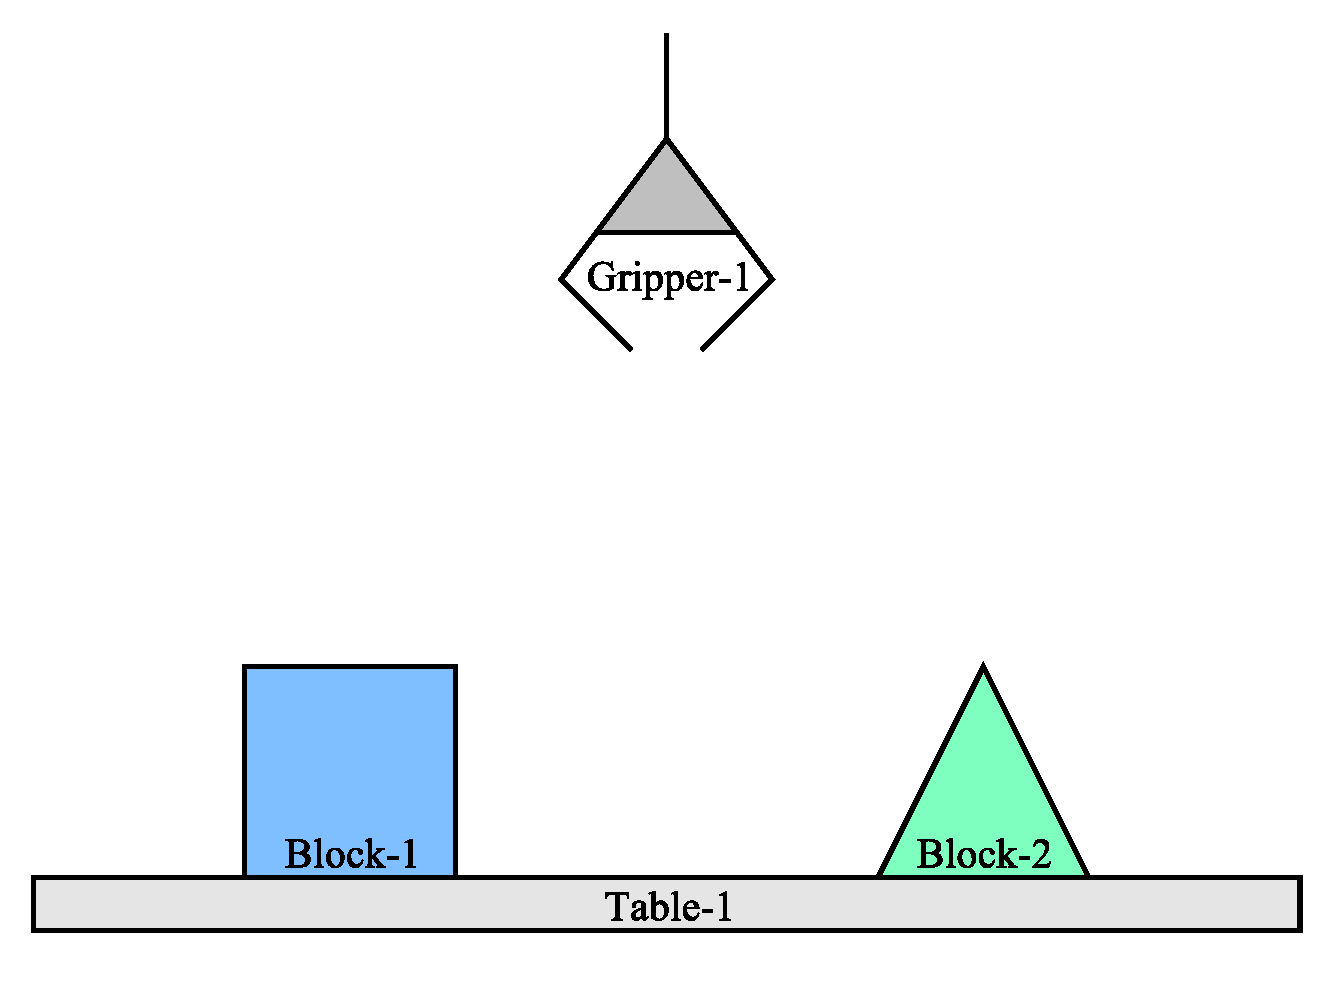
\includegraphics[width=6cm]{gfx/blocks_world_example-1}
%%   \caption[An example problem domain.]{An example problem domain.}
%%   \label{figure:an_example_problem_domain}
%% \end{wrapfigure}
%% has the goal of making a stack of two blocks.  The AI is now
%% confronted with the task of reasoning about how to get the physical
%% world into a state that matches this goal condition.  Specifically,
%% the AI must decide upon a plan of action, either creating a new plan
%% from scratch, or recalling a plan from memory that with some
%% modifications seems like it might work in this case.  When the AI
%% considers the plans that it knows, it remembers a plan that it has
%% been told will result in a stack of two blocks.  For example, the plan
%% shown in {\mbox{\autoref{table:a_plan_learned_from_being_told}}}
%% asserts that there is a stack of two blocks as its final operation.
%% If the AI were to recall this plan and execute it in the situation
%% shown in \autoref{figure:an_example_problem_domain}, the AI would
%% encounter an expectation failure at the final assertion of the
%% expected post-conditions of this plan.
%% {\mbox{\autoref{figure:failure_to_stack_cube_on_pyramid}}} shows how
%% executing this plan in this situation might fail to result in a stack
%% of two blocks: the pyramid does not support the cube, so the cube
%% falls off of the pyramid and onto the table.  In the case of a failure
%% of expectations, a refined hypothetical model of the physical world is
%% learned, so that the same planning mistake will never be made again.
%% \begin{wraptable}{l}{8cm}
%% \centering
%% \begin{tabular}{|rl|}
%% \hline
%%  1. & Move left.\\
%%  2. & Wait until a gripper is above a cube.\\
%%  3. & Reach and grab.\\
%%  4. & Wait until a gripper stops moving.\\
%%  5. & Move right.\\
%%  6. & Wait until a gripper is above a pyramid.\\
%%  7. & Drop and wait for block to fall.\\
%%  8. & Assert a cube is sitting on a pyramid.\\
%% \hline
%% \end{tabular}
%% \caption[A plan learned from ``being told''.]{A plan learned from
%%   ``being told''.}
%% \label{table:a_plan_learned_from_being_told}
%% \end{wraptable}
%% In my AI, learning a new physical model of the world amounts to
%% relearning the hypotheses for the expected transframes that result
%% from executing different physical actions, leading from one collection
%% of physical situation type events to another.  In this case, the AI
%% learns many new refined hypotheses about the physical world.  For
%% example, the AI learns that executing the action of moving to the left
%% until a cube is below the gripper results in a cube being below the
%% gripper.  Of course, this may not generally be true, but the AI's
%% physical action hypotheses are refined in light of this added
%% experiential knowledge that predicts this change given the specific
%% preconditions.  The AI still retains many hypotheses that leave room
%% for the possibility that executing this action in other preconditions
%% may or may not result in this specific change.  For example, at this
%% point, the AI has no experience executing this action when there is
%% not a block to the left of the gripper.  In that case, the AI cannot
%% be sure that this action will result in a block being below the
%% gripper, and this uncertainty is represented in the hypothesis space
%% of the AI's concept learning algorithm.

%% In addition to learning a refined hypothetical model of the physical
%% world, the AI also learns a better model of how to control its
%% planning machine that chose this plan for some reason and decided to
%% execute it.  In other words, not only has the AI failed to act
%% physically but also the AI has failed in thinking about its plans.
%% The AI decided to execute a plan that ended up failing.  Because the
%% AI has a reflective learning algorithm, it has the additional ability
%% to learn a better model of the planning process itself---the planning
%% process that selected this plan, imagined its physical effects, and
%% decided to execute it.

%% Deliberative planning processes are plans of the reflective
%% metacognitive reasoning layer.  The reflective layer contains a
%% metacognitive planning machine that creates, reasons about, and
%% executes plans for how to control the deliberative planning machine.
%% Thus, the AI has two layers of planners: one planner that learns about
%% physical processes and another planner that learns about planning
%% processes.  A plan for physical action is manipulated by resources in
%% the deliberative layer, while a plan for deliberative action is
%% manipulated by resources in the reflective layer.

%% In this example, the goal of the reflective planning machine is to
%% attempt to avoid plan execution failures, while executing plans that
%% are hypothesized to accomplish physical goals.  The plan executed in
%% the deliberative planner resulted in a physical expectation failure.
%% The plan attempted to assert that a cube is supported by a pyramid,
%% which was not true at the point when the assertion was executed in the
%% deliberative planning machine.  When a plan encounters a specific type
%% of failure, properties of the failure event are represented as a
%% failure object that is associated with the plan object that failed.
%% As seen by the reflective layer, the deliberative failure knowledge is
%% related to the plan in a way that is analogous to the way that the
%% deliberative layer sees a physical block sitting on another physical
%% block.  The deliberative layer learns how to control relationships
%% between physical objects, while the reflective layer learns how to
%% control relationships between deliberative objects, such
%% \begin{figure}{h}
%%   \centering
%%   \begin{tabular}{p{5cm}p{5cm}}
%%     1. 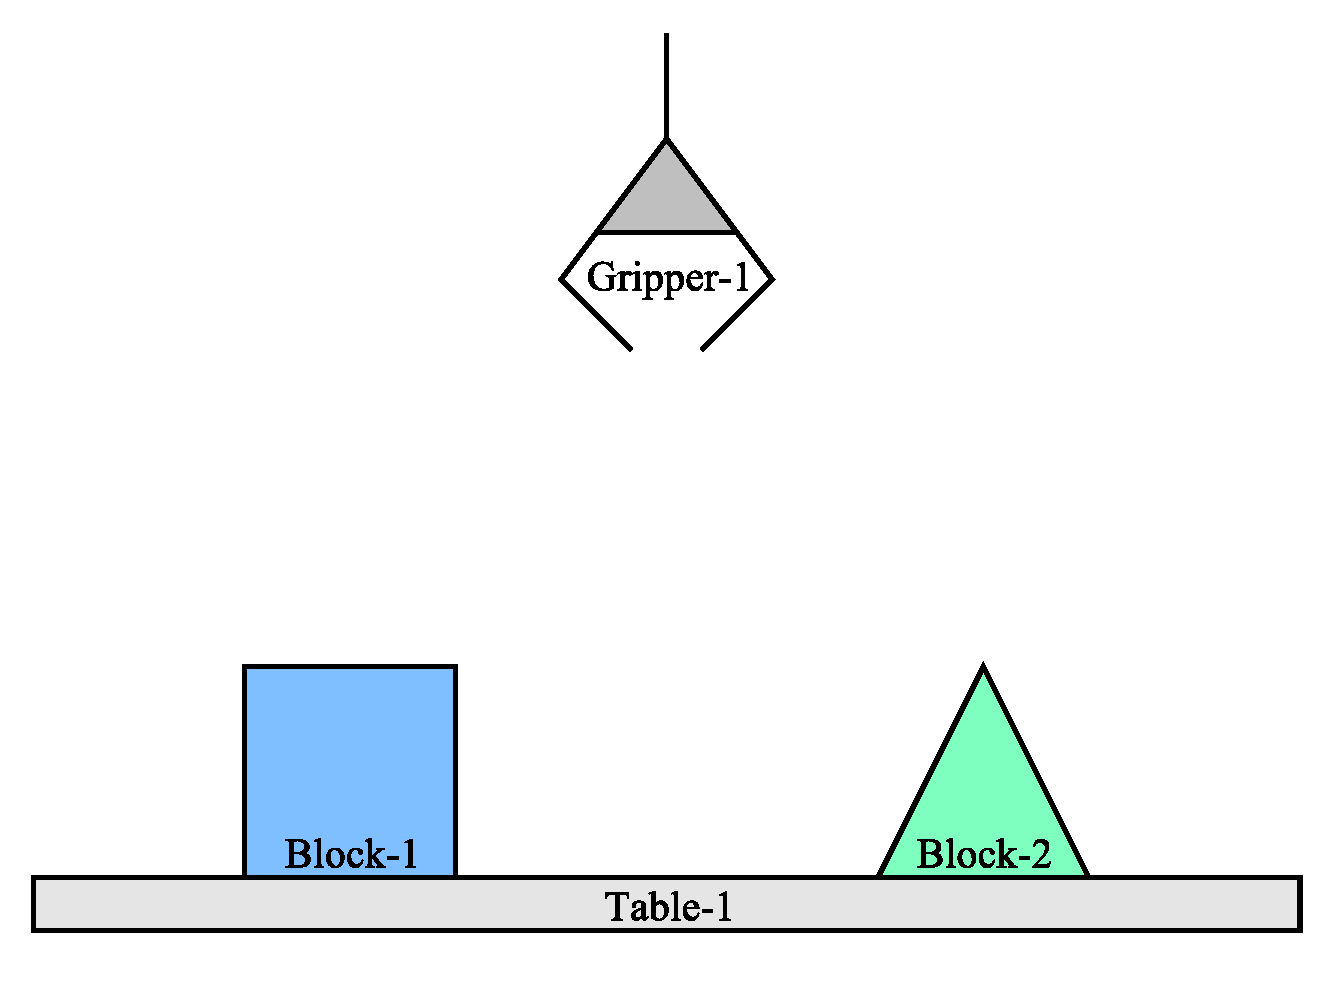
\includegraphics[width=5cm]{gfx/blocks_world_example-1}  & 2. 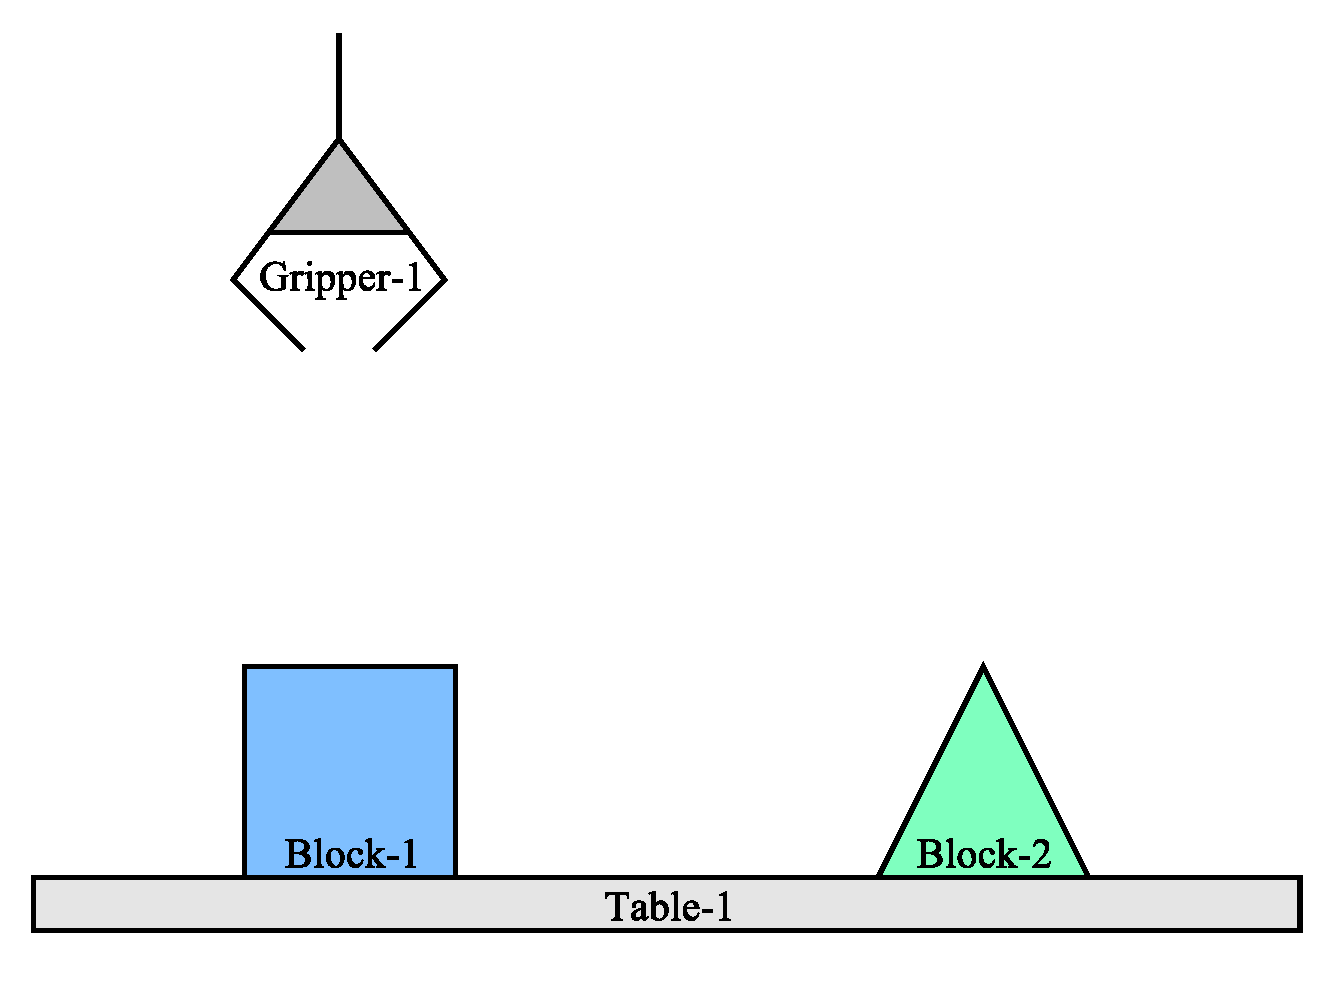
\includegraphics[width=5cm]{gfx/blocks_world_example-2} \\
%%     3. 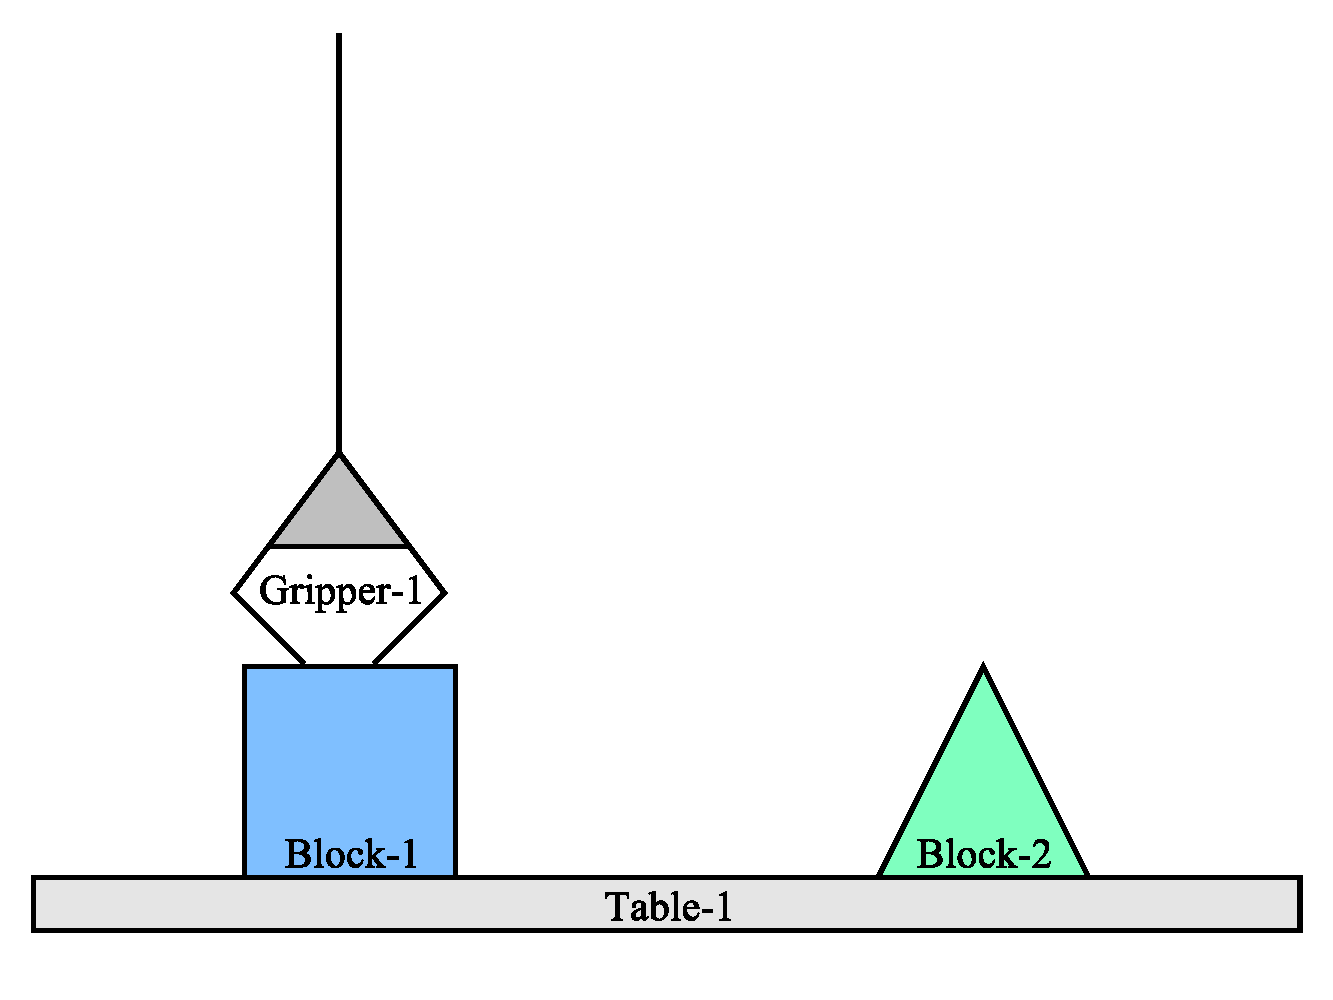
\includegraphics[width=5cm]{gfx/blocks_world_example-3}  & 4. 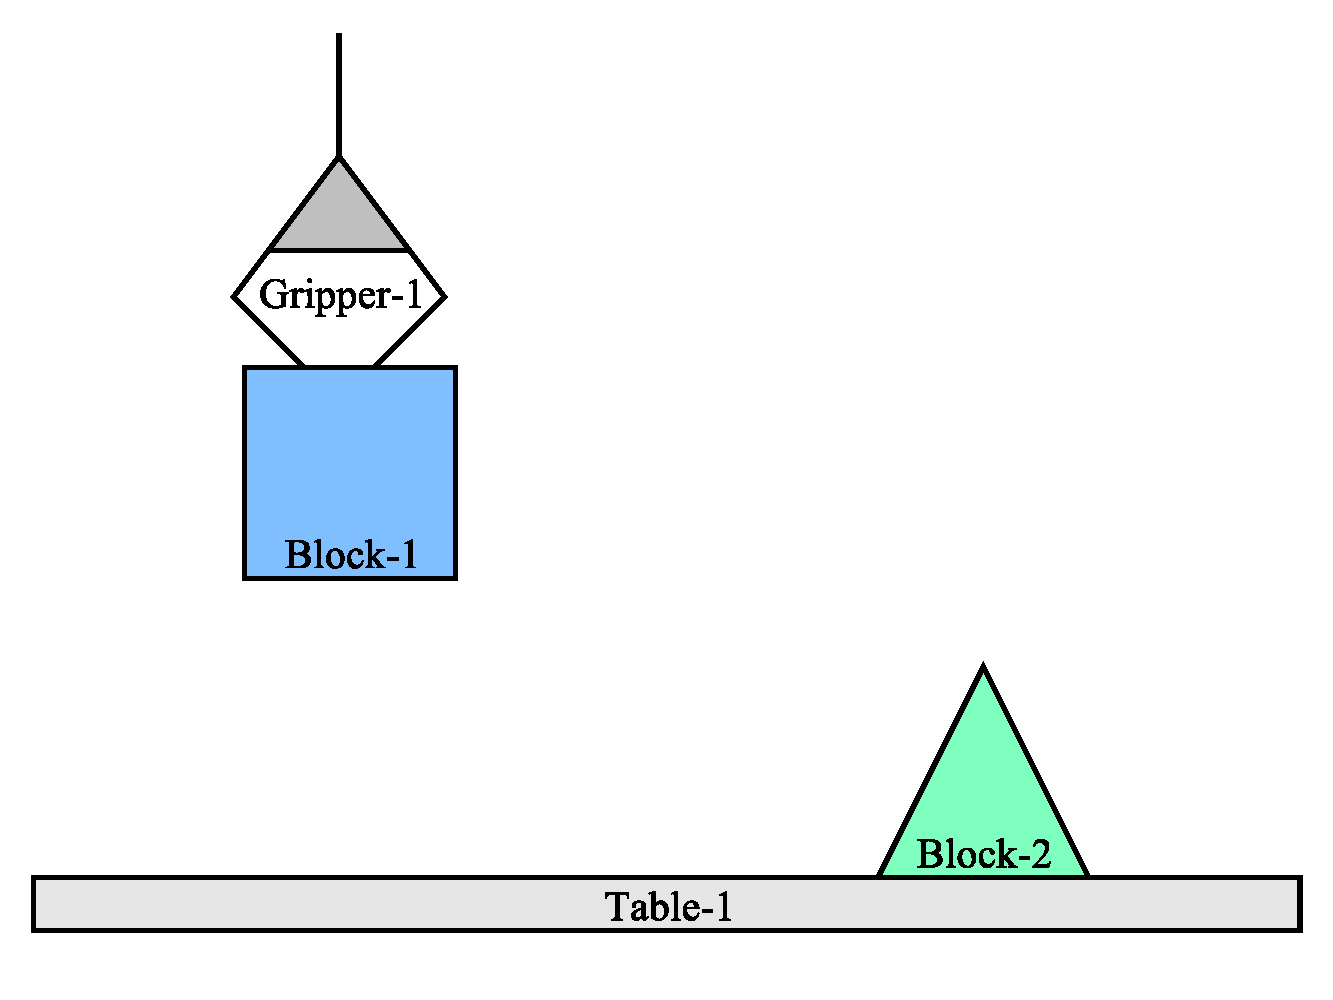
\includegraphics[width=5cm]{gfx/blocks_world_example-4} \\
%%     5. 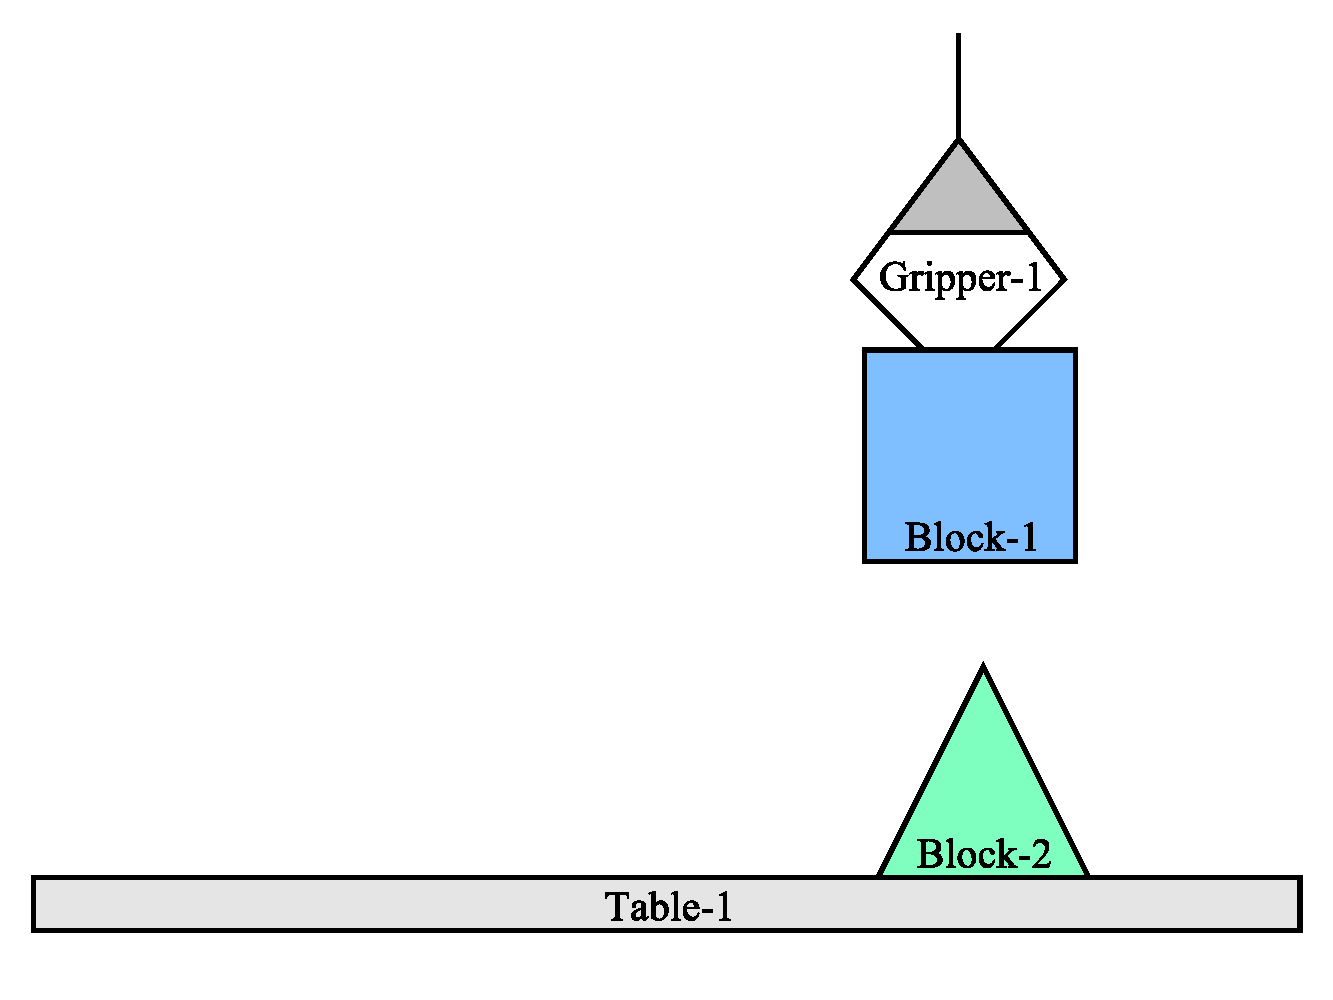
\includegraphics[width=5cm]{gfx/blocks_world_example-5}  & 6. 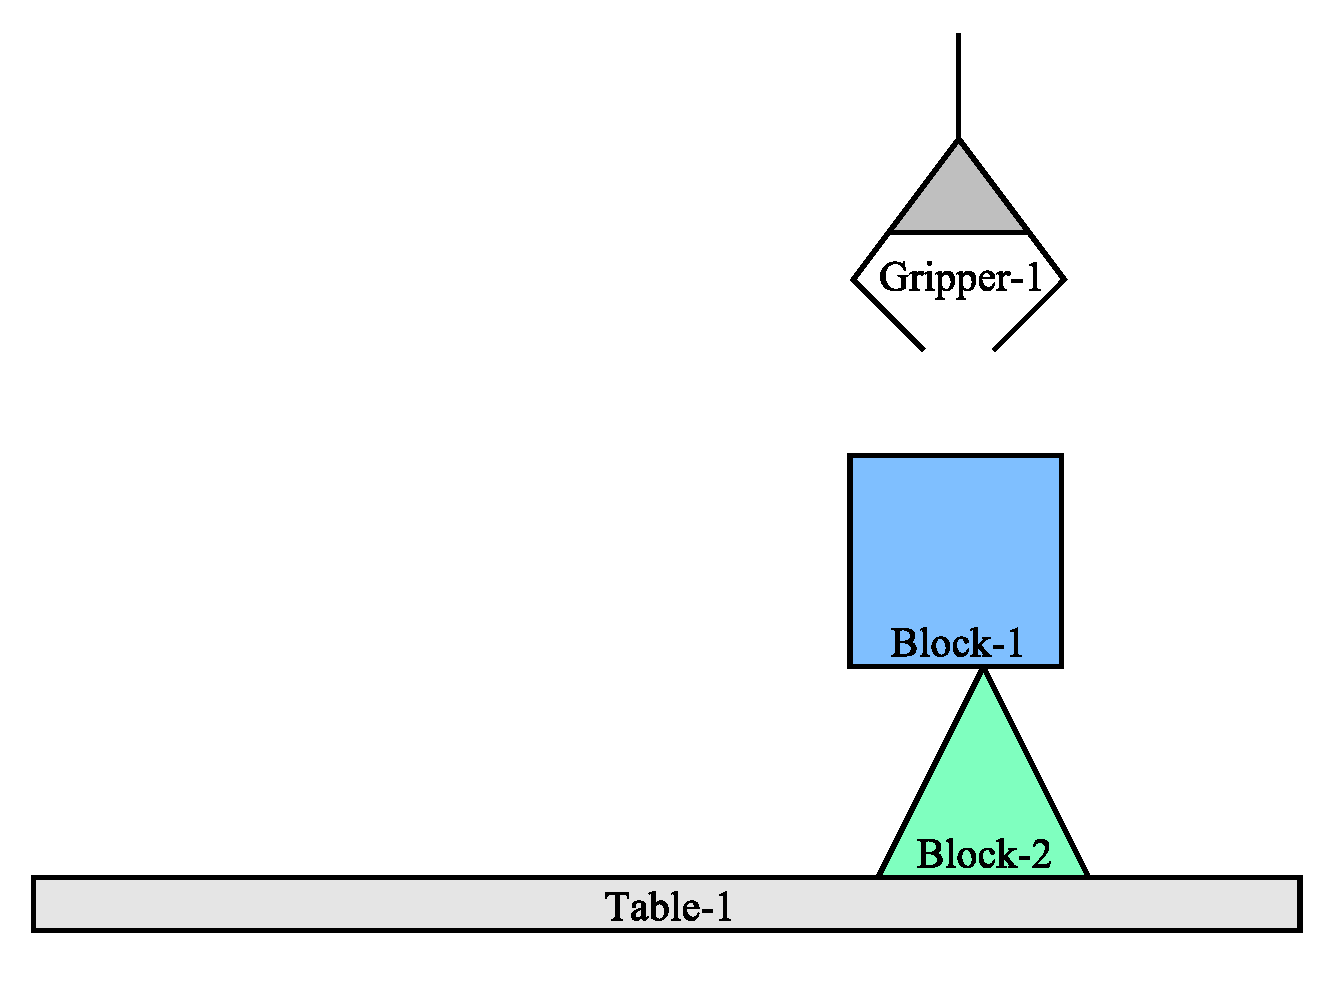
\includegraphics[width=5cm]{gfx/blocks_world_example-6} \\
%%     7. 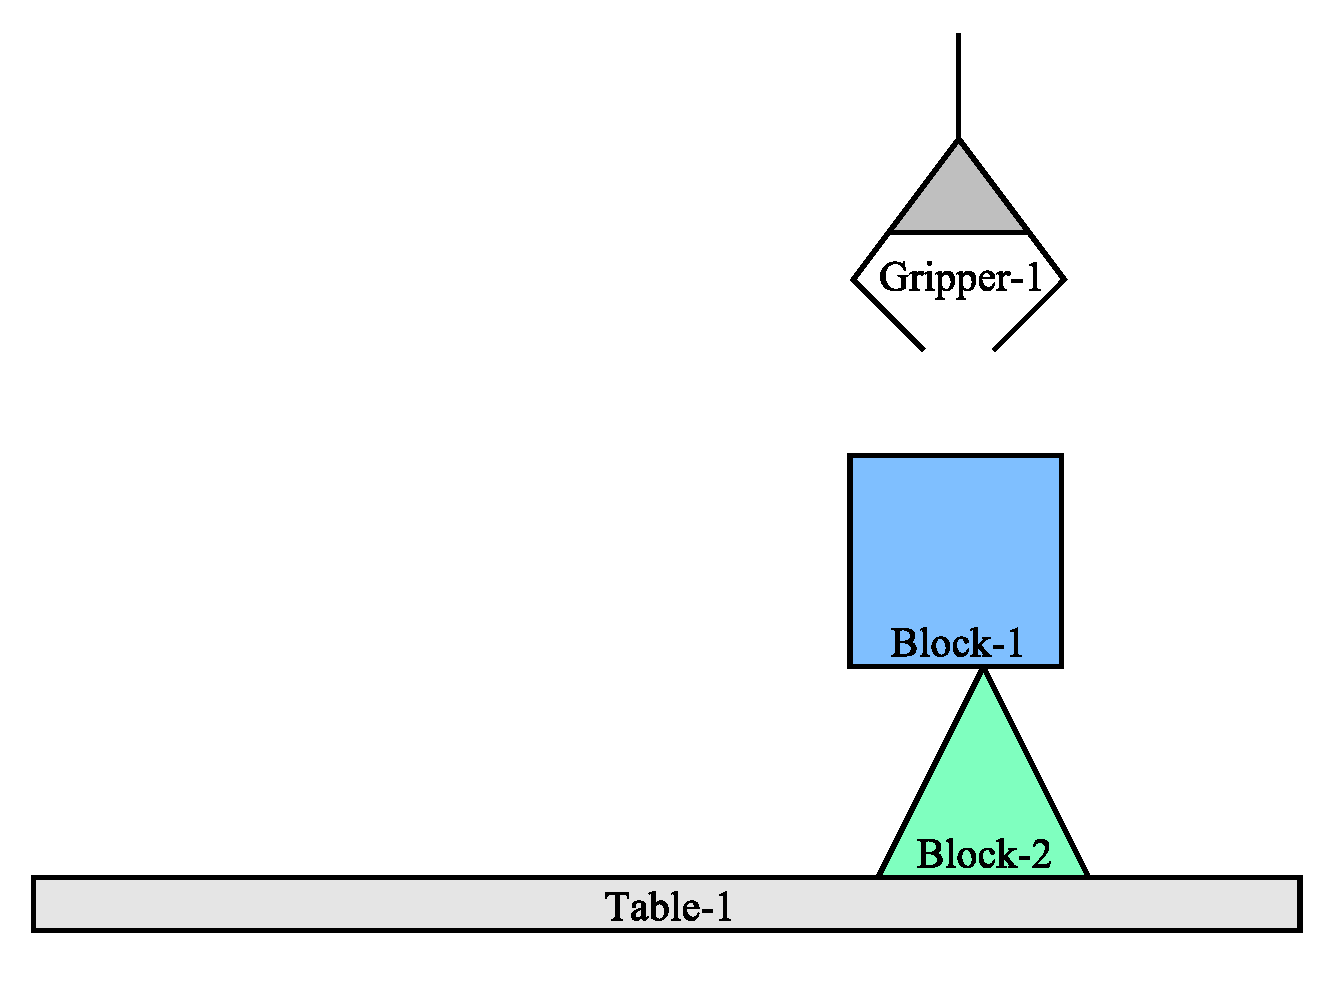
\includegraphics[width=5cm]{gfx/blocks_world_example-7}  & 8. 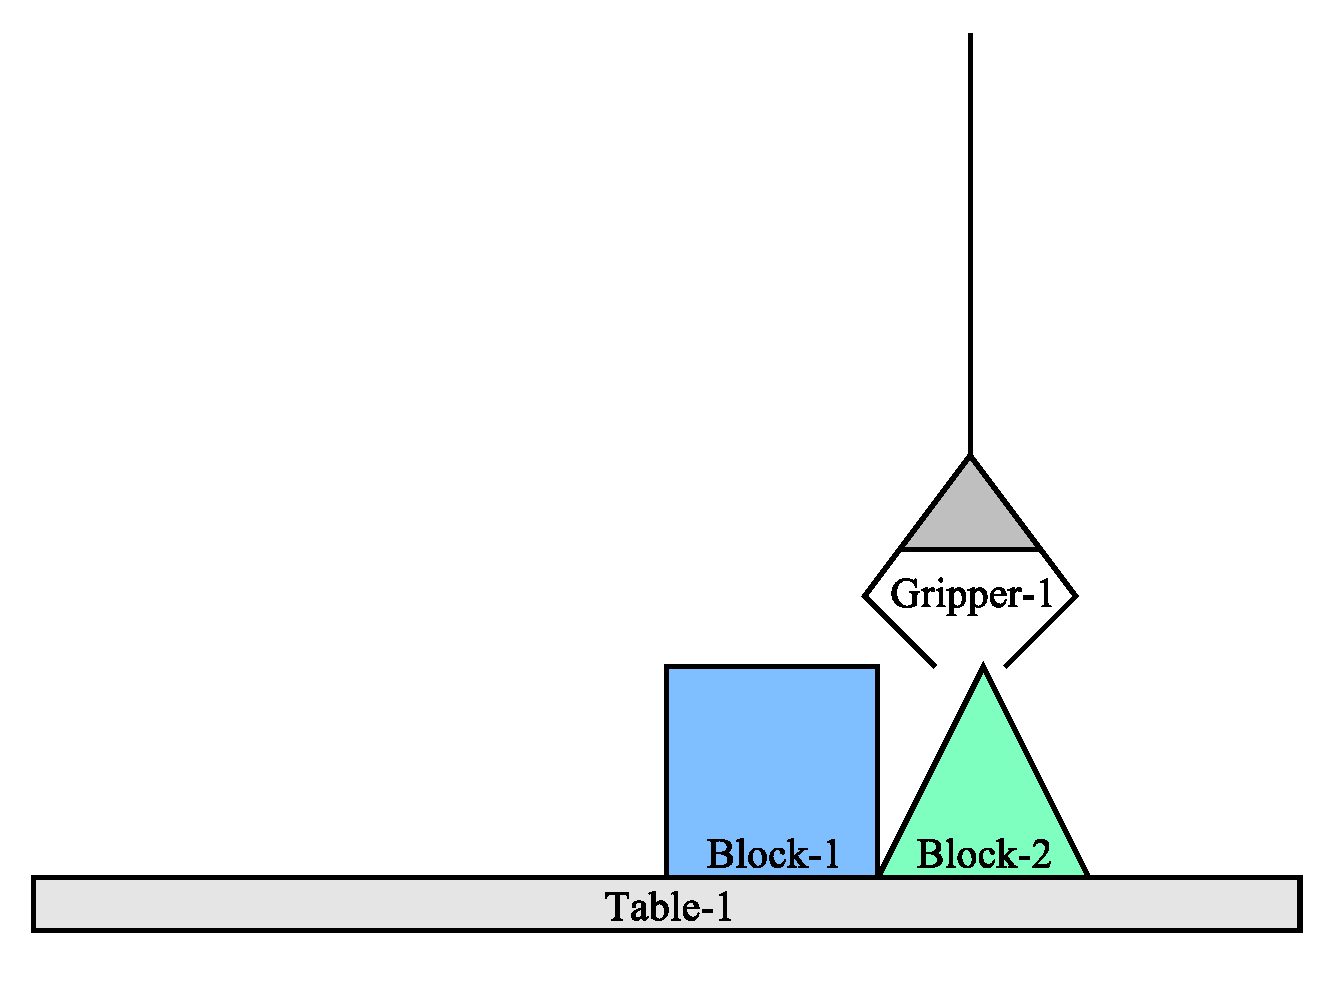
\includegraphics[width=5cm]{gfx/blocks_world_example-8}
%%   \end{tabular}
%%   \caption[An example of an expectation failure.]{An example of an
%%     expectation failure.  A plan is executed that asserts that a
%%     post-condition must be a stack of a cube sitting on a pyramid,
%%     but when the plan finishes executing this assertion fails.}
%%   \label{figure:failure_to_stack_cube_on_pyramid}
%% \end{figure}
%% as the deliberative planning machine, plans, hypotheses, and execution
%% failures.

%% The reflective layer learns models of how deliberative actions change
%% the types of knowledge relationships between objects in the
%% deliberative layer.  The reflective planning machine attempts to
%% accomplish deliberative type knowledge goals computed from this
%% deliberative knowledge.  Here is a list of deliberative type knowledge
%% that the reflective layer can know about the objects in the
%% deliberative layer:
%% \begin{itemize}
%% \item A plan that asserts that a cube is sitting on a pyramid is
%%   under the focus of the deliberative planning machine.
%% \item A plan that has had an expectation failure is being executed by
%%   the deliberative planning machine.
%% \item There is no plan currently executing in the deliberative
%%   planning machine.
%% \item There is a plan to drop a block that you are holding before
%%   reaching and grabbing.
%% \item The deliberative planning machine is focused on a plan to move
%%   to the left while concurrently moving to the right.
%% \end{itemize}
%% These types of states are learned in the reflective layer by
%% processing a procedurally reflective event stream generated by the
%% deliberative layer planning processes.  These types of states are
%% potential goals, preconditions, and effects in the reflective planning
%% machine that models how deliberative actions effect the types of
%% states in the deliberative planning-machine knowledge.  Reflective
%% hypotheses about the deliberative layer are learned in terms of these
%% types of states.  The reflective layer learns hypotheses for
%% predicting types of plan execution failure knowledge from other
%% deliberative types of knowledge preconditions.

%% In the example, executing the plan that the deliberative planner is
%% focused on is hypothesized to result in a plan having an expectation
%% failure event.  The reflectively planned execution of the deliberative
%% execution of the plan is processed concurrently with the deliberative
%% planning machine operations, slightly behind the times, not
%% necessarily slowing down the deliberative planning resources.  The
%% reflective layer induces deliberative types of knowledge from this
%% reflectively reconstructed deliberative planning machine knowledge
%% base.  The preconditions and effects of the deliberative execution
%% actions are learned from the types of this reflective reconstruction,
%% learning to predict, in terms of types of knowledge, the effects of
%% planning actions on plans in general.  In the example, these types of
%% knowledge include: ``The plan currently under focus contains an
%% assertion that a cube must be stacked on a pyramid.''  The AI refines
%% many of its hypotheses given this limited experience of failure,
%% retaining the hypothesis that executing the plan under focus might
%% result in failure due to the plan's assertion that a cube is sitting
%% on a pyramid.

%% {\mbox{\autoref{figure:implemented_example_learning_storyboard}}}
%% shows an example of how reflectively learning about the deliberative
%% planning machine can lead to the successful achievement of a physical
%% goal.  In this example, the reflective layer infers the results of
%% executing plans and tries to predict their failure based on the
%% structure of the plan and its relationship to other deliberative
%% knowledge, such as different types of failure events.
%% {\mbox{\autoref{table:a_metacognitive_plan_learned_from_being_told}}}
%% shows an example metacognitive plan that the reflective layer is
%% executing in order to control the deliberative planning machine.
%% Based on these planned resource executions from the reflective layer,
%% the deliberative layer recalls a plan from memory that it has ``been
%% told'' but does not have experience executing.
%% \begin{wraptable}{l}{8cm}
%% \centering
%% \begin{tabular}{|rl|}
%% \hline
%%  1. & While no plans for goal, repeat 2--7.\\
%%  2. & ~~Forget all imagined events.\\
%%  3. & ~~Set imagine time to be now.\\
%%  4. & ~~Imagine current situation.\\
%%  5. & ~~Recall plan from memory.\\
%%  6. & ~~Imagine executing plan in focus.\\
%%  7. & ~~Check goals in imagination.\\
%%  8. & Recall plan for goal.\\
%%  9. & Execute plan in focus.\\
%% \hline
%% \end{tabular}
%% \caption[A metacognitive plan in the reflective layer learned from
%%   ``being told''.]{A metacognitive plan in the reflective layer
%%   learned from ``being told''.}
%% \label{table:a_metacognitive_plan_learned_from_being_told}
%% \end{wraptable}
%% The reflective layer imagines executing the plan for deliberation in
%% terms of the planning machine of the deliberative layer.  The
%% reflective layer imagination does not include physical effects of
%% physical actions.  The reflective layer only learns from and predicts
%% the types of knowledge in the deliberative layer, such as the
%% properties and relationships between the planning machine, plans, and
%% failure events.  Because of the AI's lack of experience, the
%% reflective layer does not infer that this plan for physical action
%% will lead to a failure in the deliberative planning machine based on
%% its structure.  Further, because of the AI's inexperience with
%% physical actions, when it reflectively decides to execute this
%% deliberative plan, it deliberatively infers that this plan will
%% actually create a stack of two blocks.  Both of these forms of
%% ignorance are corrected when the AI attempts to execute the chosen
%% plan.  Not only is a new model of the physical world learned but also
%% a new model of the deliberative planning machine is learned by the
%% reflective layer.  In this way, the failure to predict the effects of
%% physical actions can also be considered a failure to predict the
%% effects of deliberative actions.  In other words, the reflective layer
%% made a mistake in controlling the planning machine by having it
%% execute a plan that ended up failing.  In general, the reflective goal
%% to control the deliberative machine to avoid execution failures is not
%% absolutely necessary.  In other situations it may be desirable for
%% physical failures to occur.  For example, if the AI is performing an
%% experiment or ``playing'' in a physical domain, it may be desirable to
%% fail in order to accomplish knowledge level goals.  In this example,
%% the reflective planner has a negative goal, which is: ``Avoid
%% Deliberative-Planner-1 just having had an execution failure.''
%% \begin{figure}
%% \centering
%% \begin{tabular}{p{3.5cm}p{3.5cm}p{3.5cm}}
%% 1. 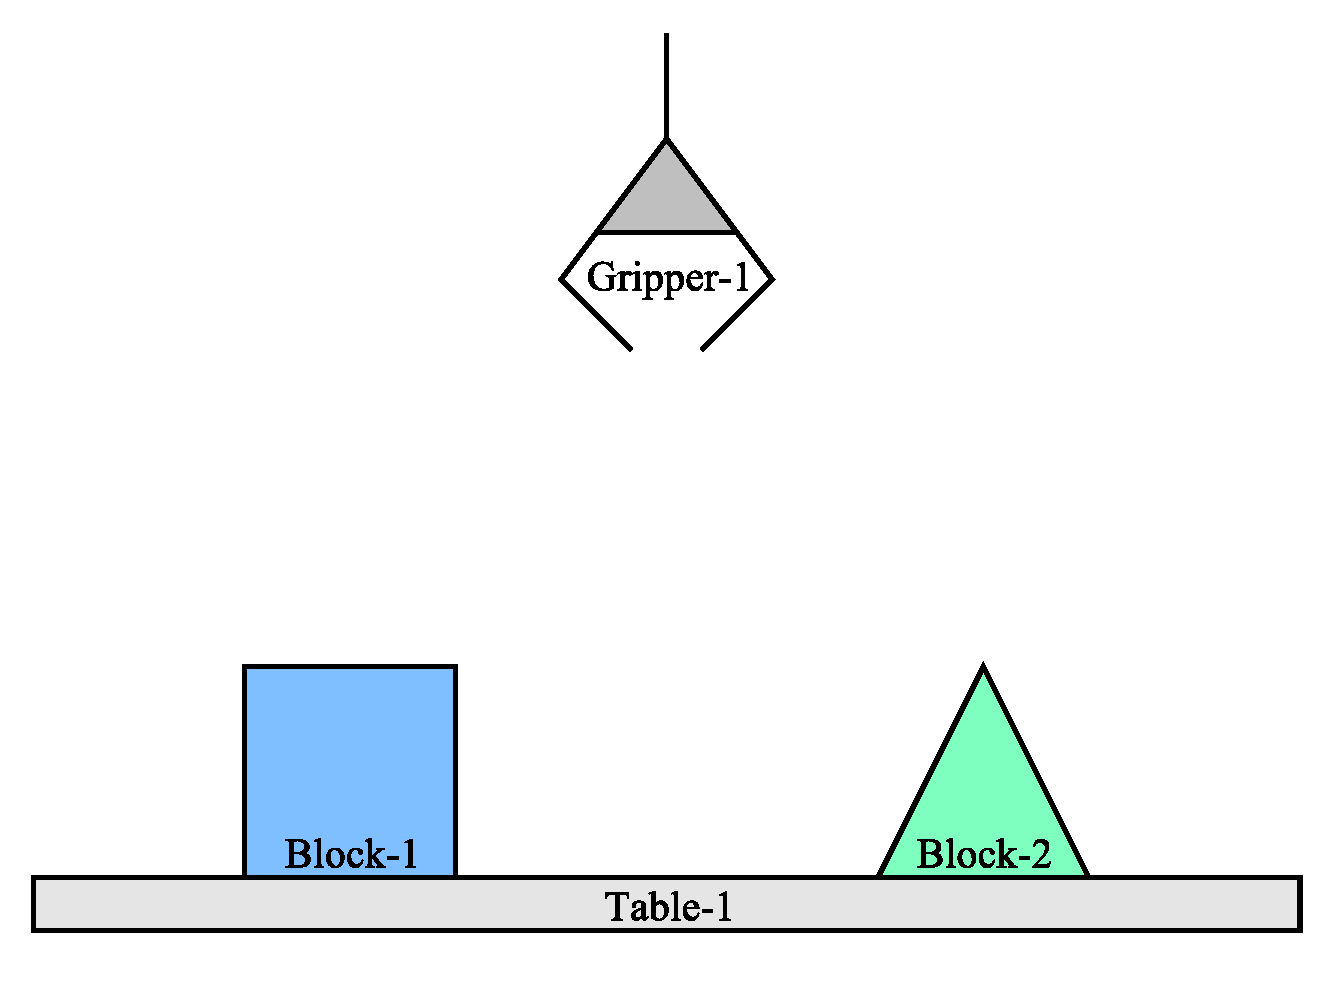
\includegraphics[width=3.5cm]{gfx/blocks_world_example-1}  & 2. 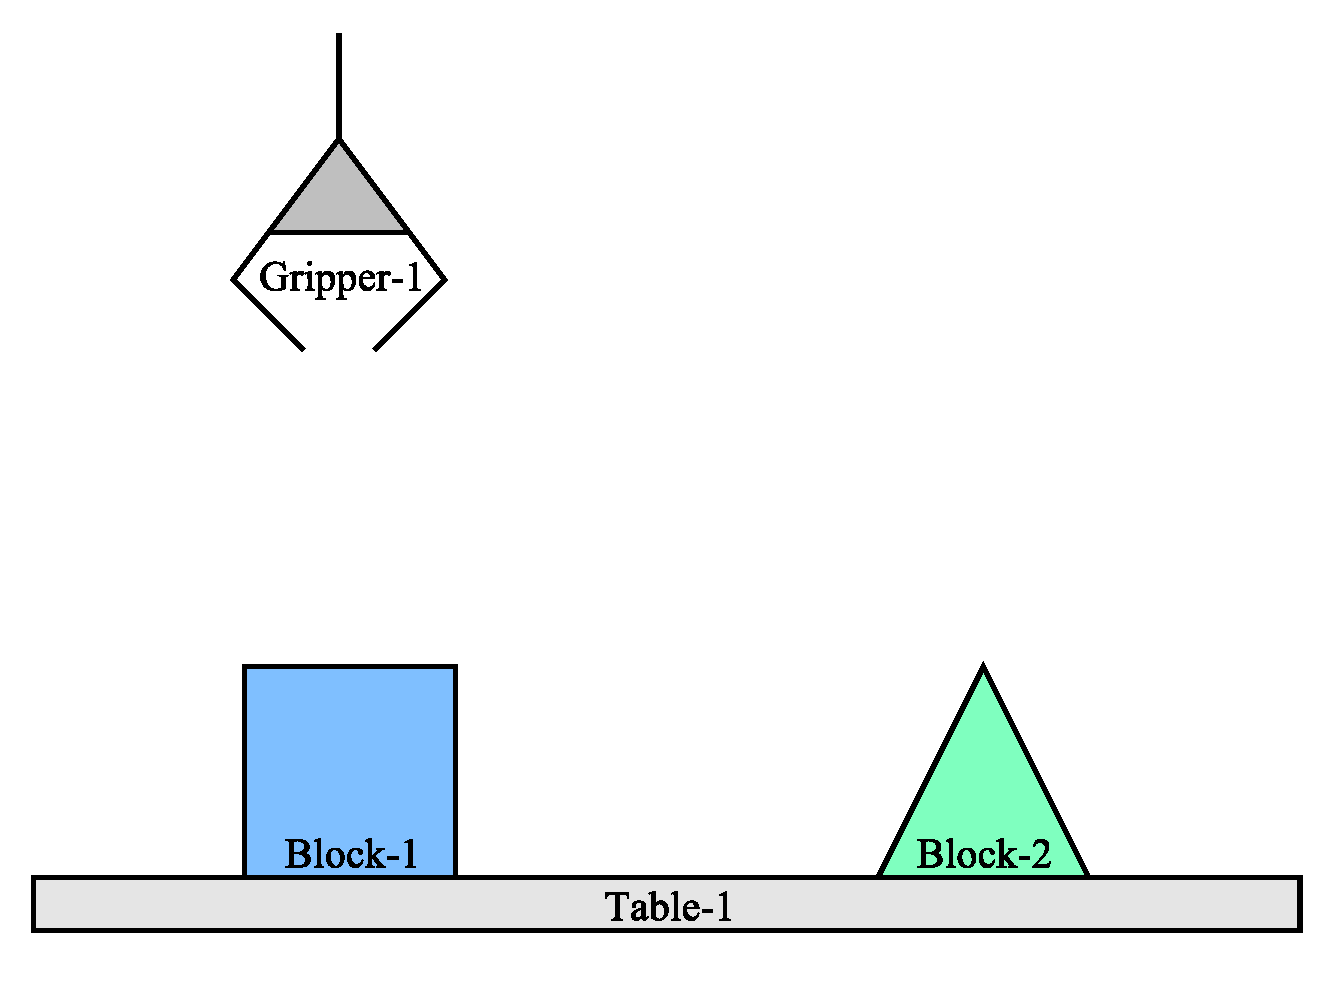
\includegraphics[width=3.5cm]{gfx/blocks_world_example-2}  & 3. 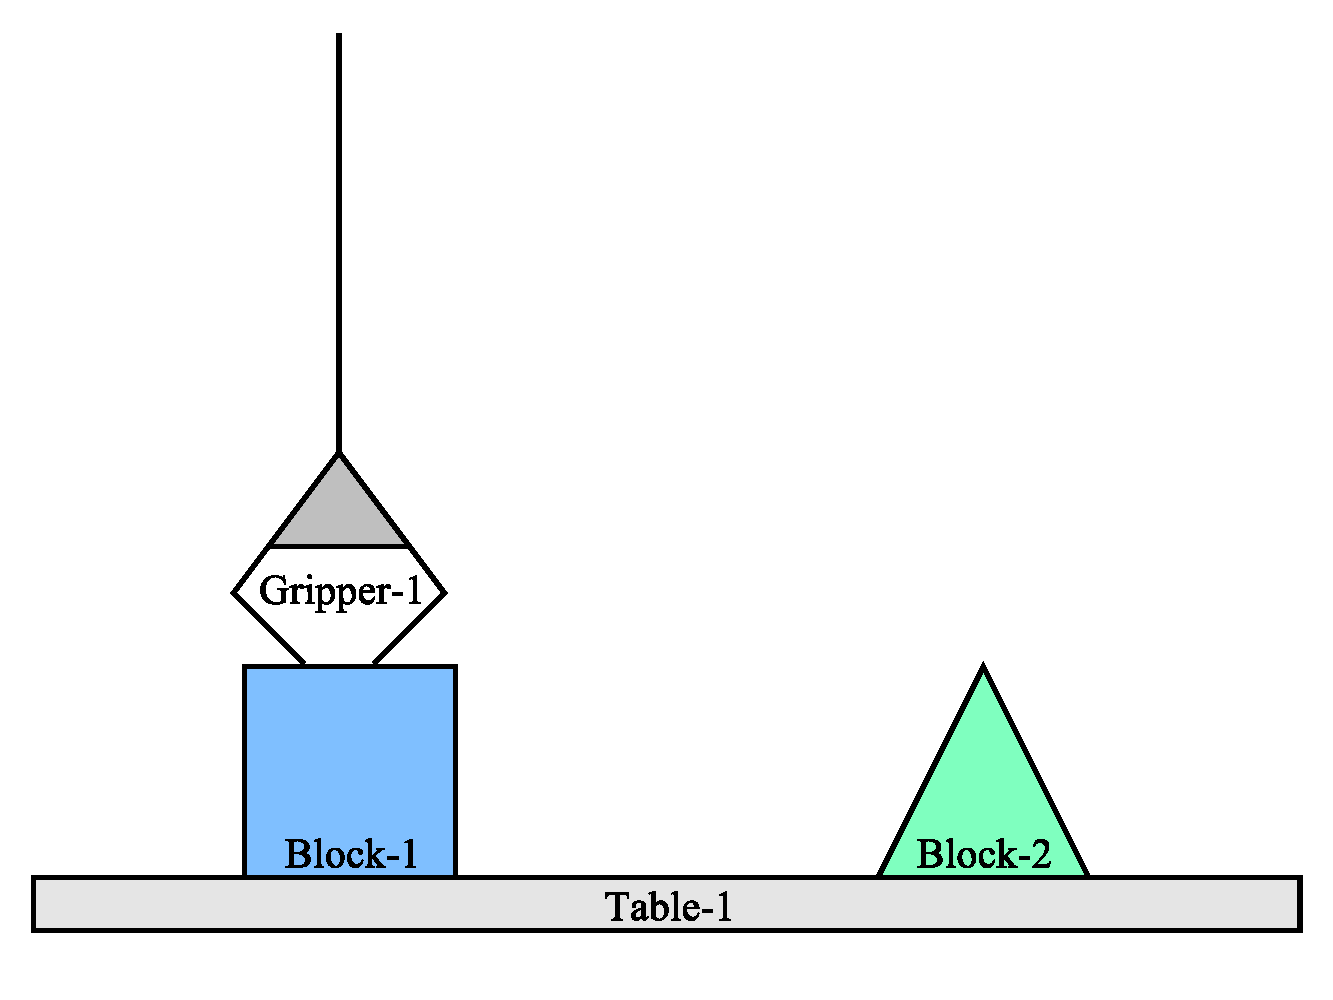
\includegraphics[width=3.5cm]{gfx/blocks_world_example-3} \\
%% 4. 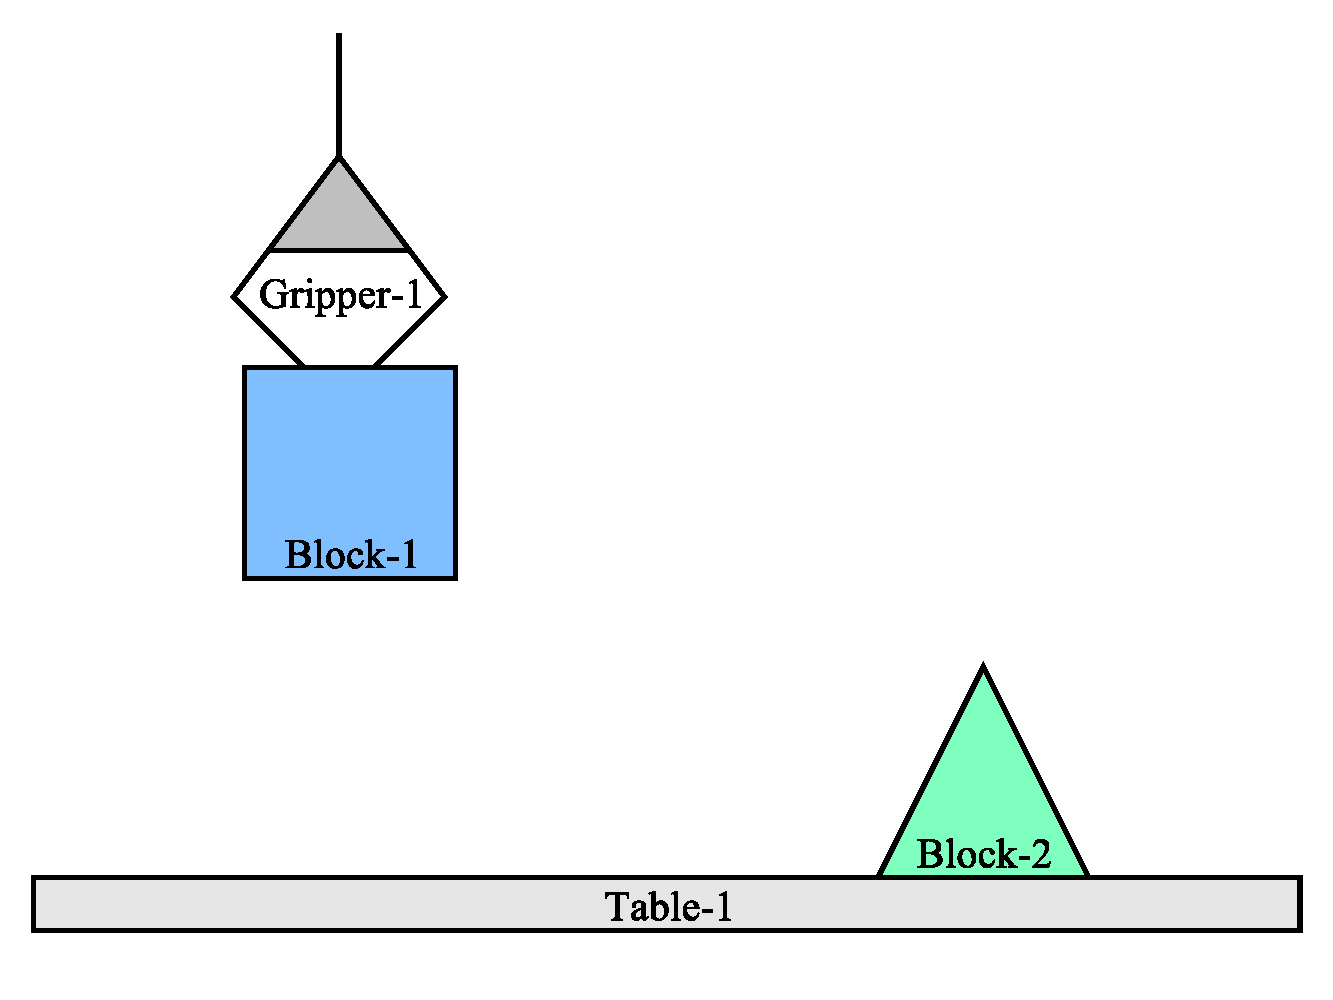
\includegraphics[width=3.5cm]{gfx/blocks_world_example-4}  & 5. 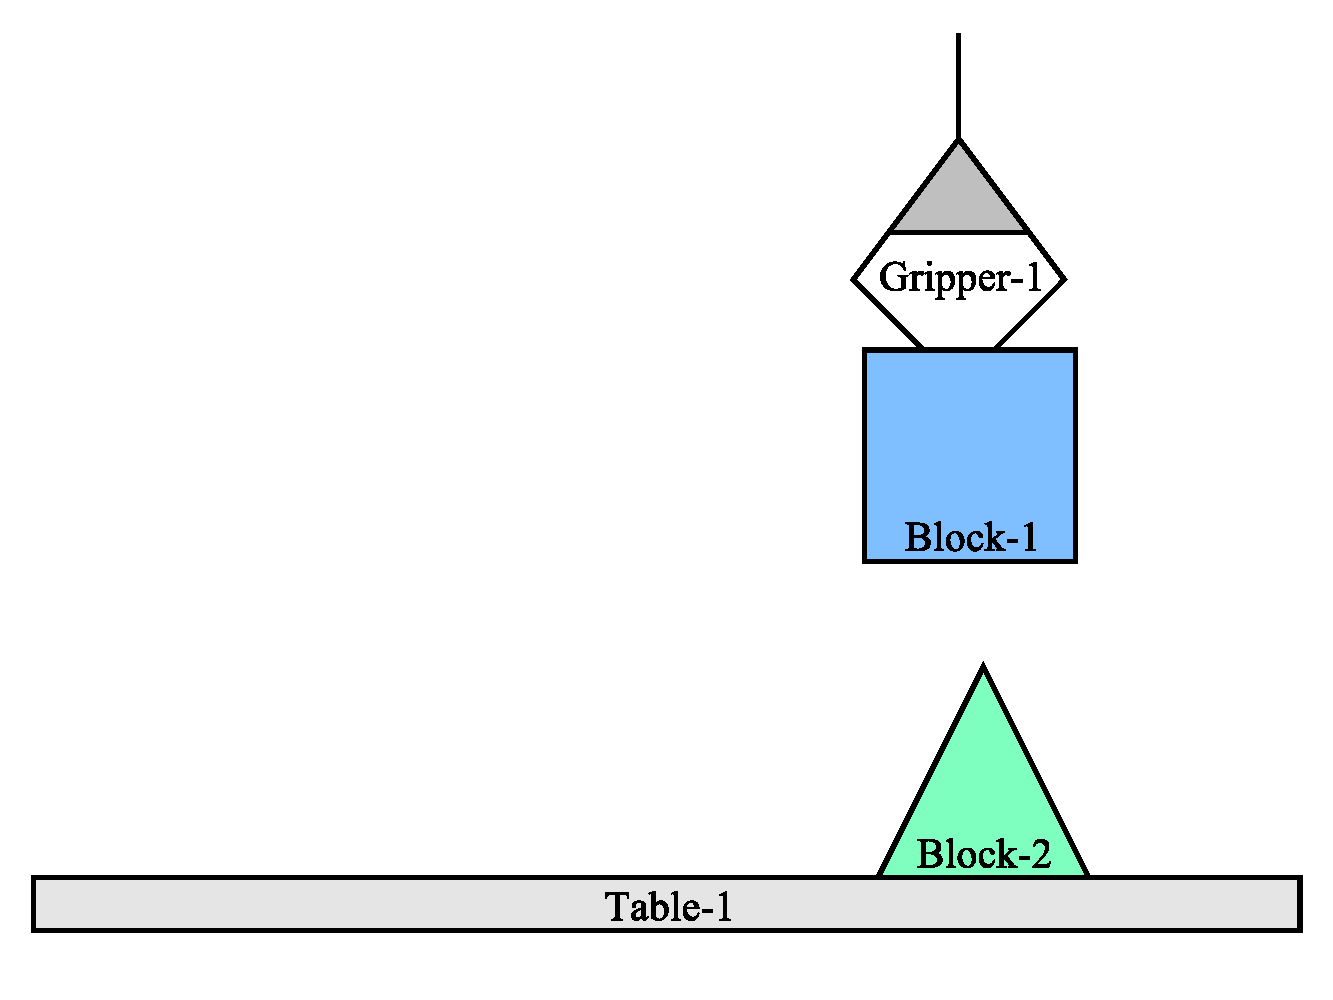
\includegraphics[width=3.5cm]{gfx/blocks_world_example-5}  & 6. 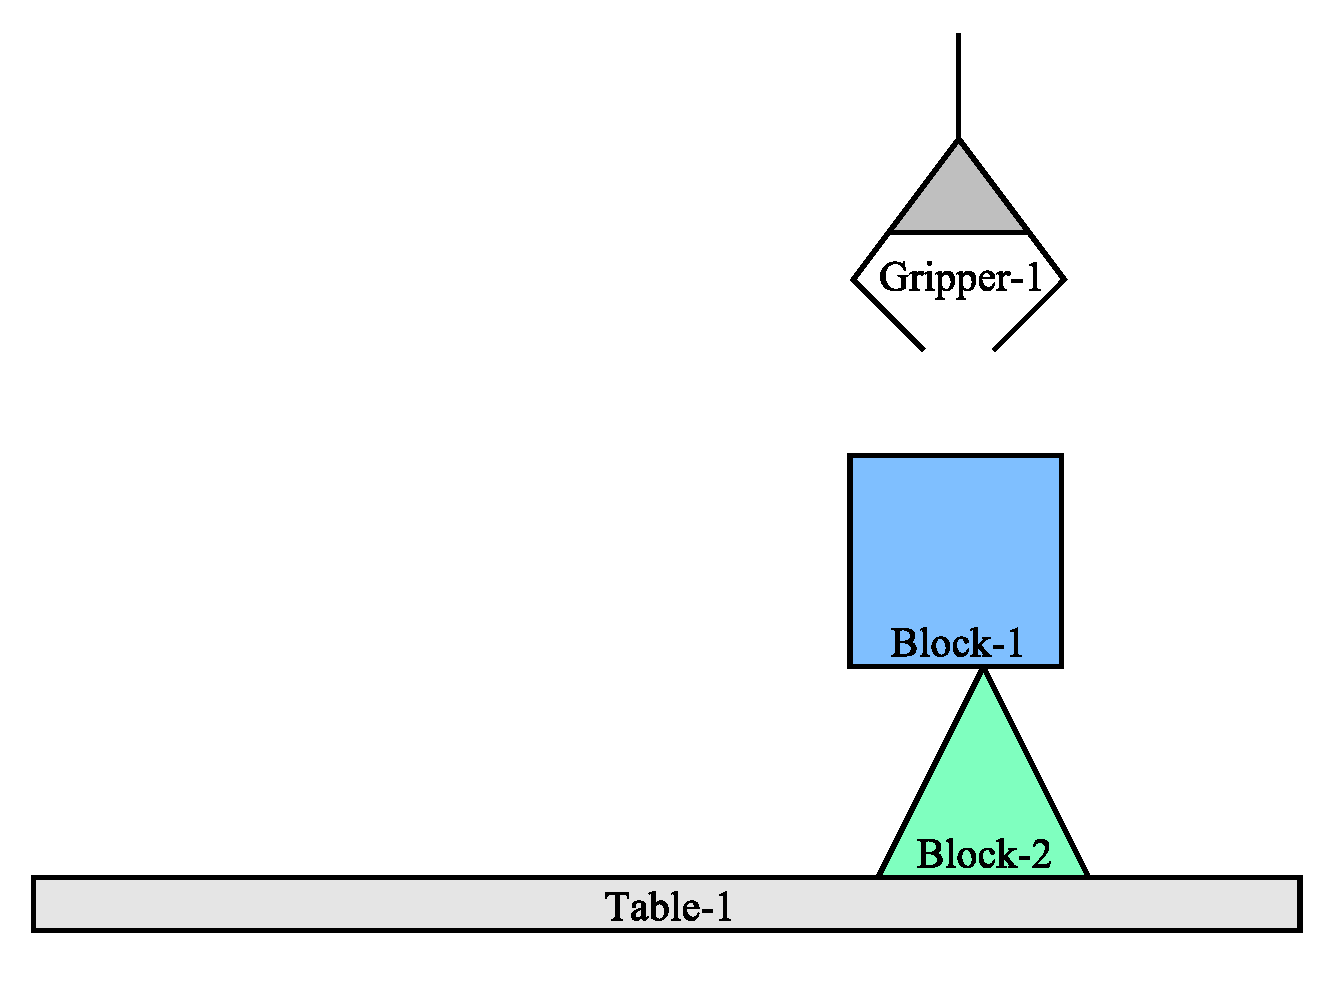
\includegraphics[width=3.5cm]{gfx/blocks_world_example-6} \\
%% 7. 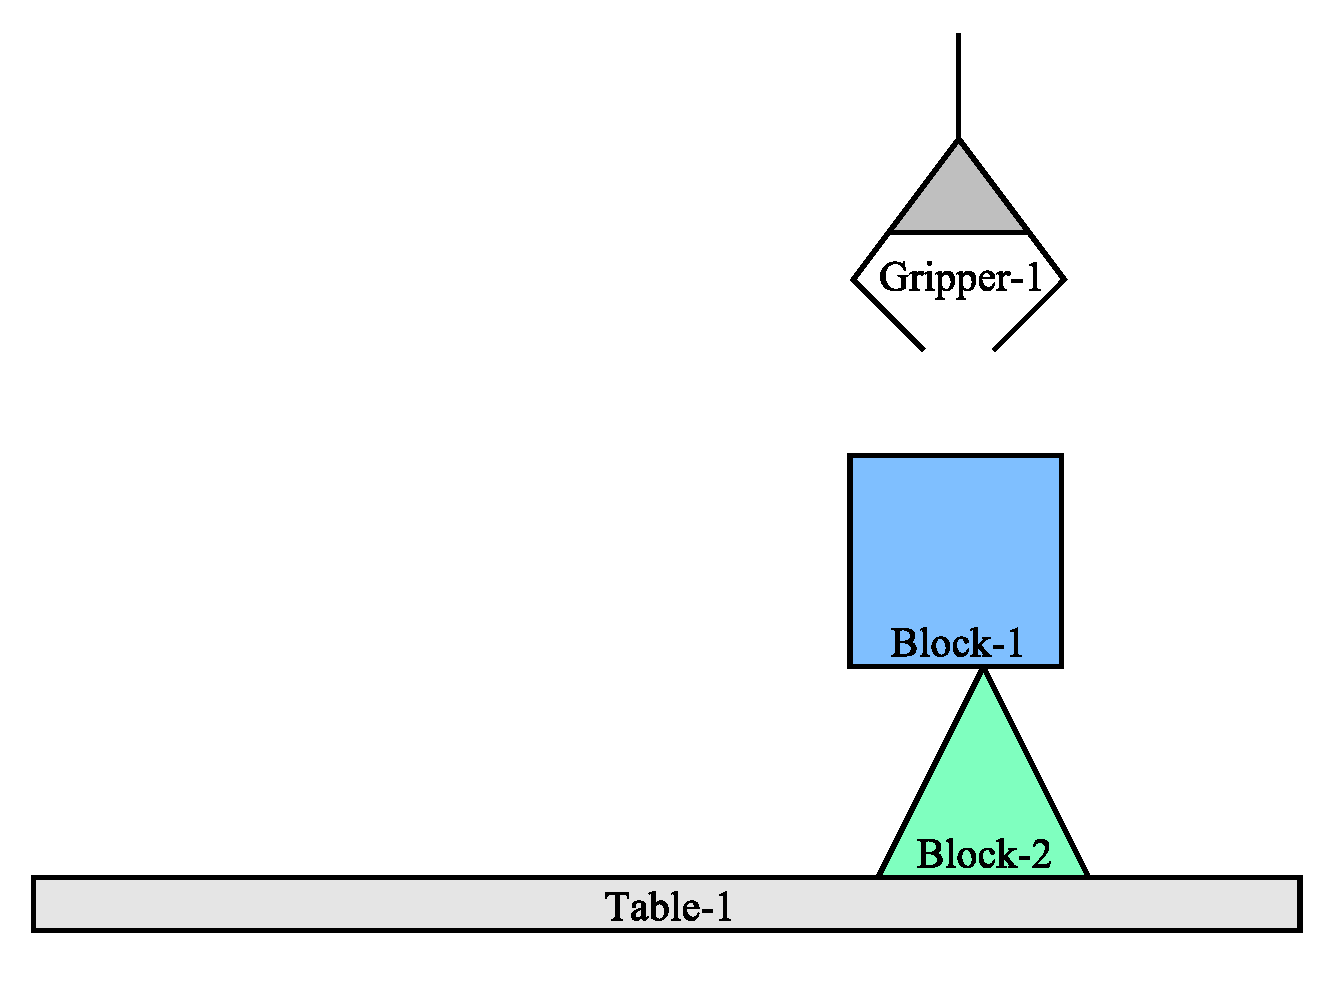
\includegraphics[width=3.5cm]{gfx/blocks_world_example-7}  & 8. 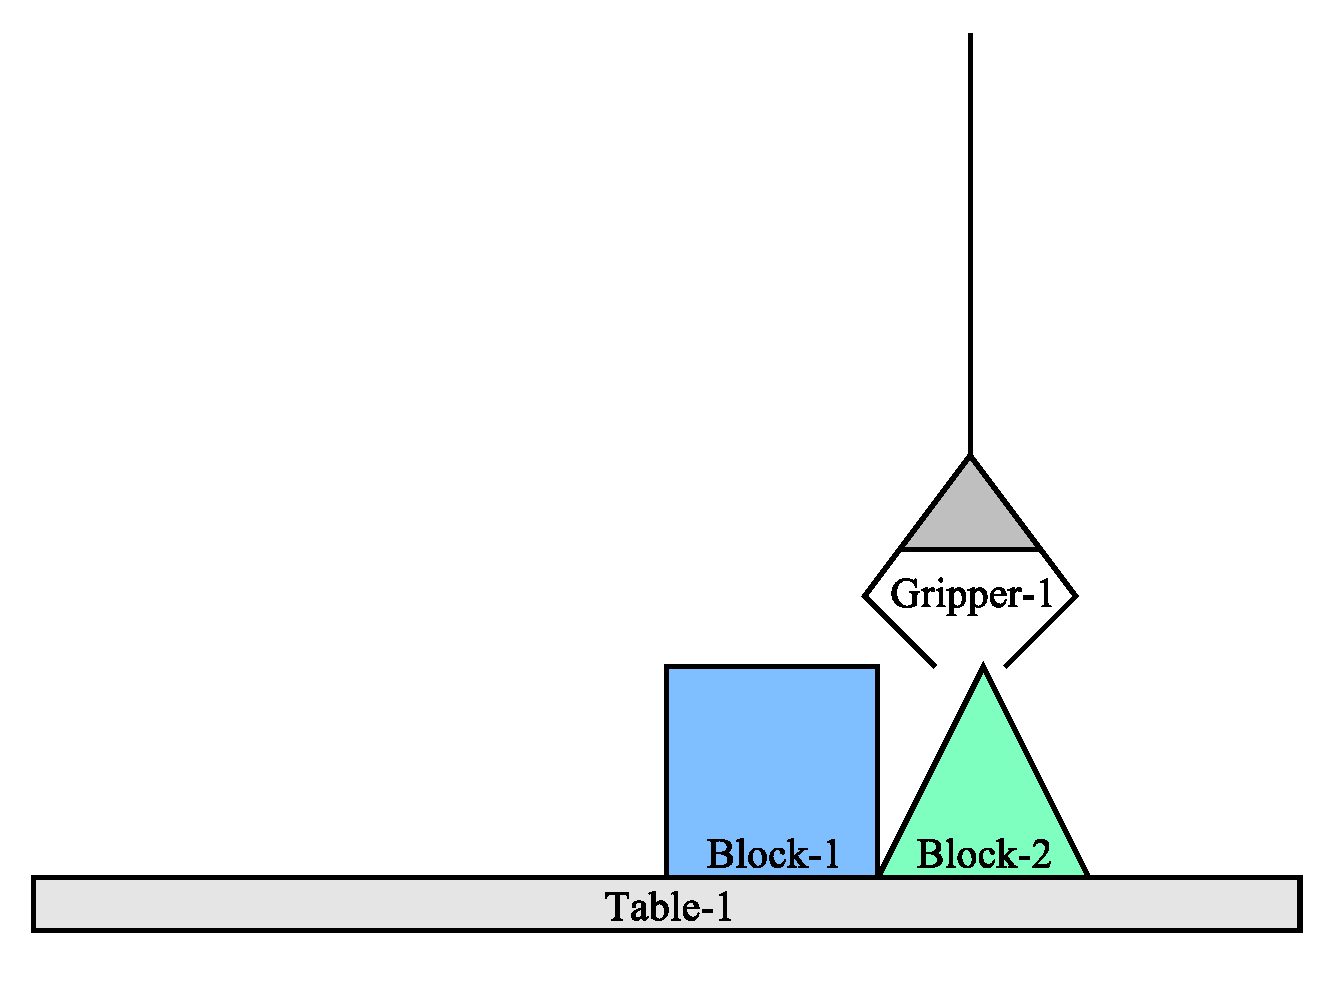
\includegraphics[width=3.5cm]{gfx/blocks_world_example-8}  & 9. 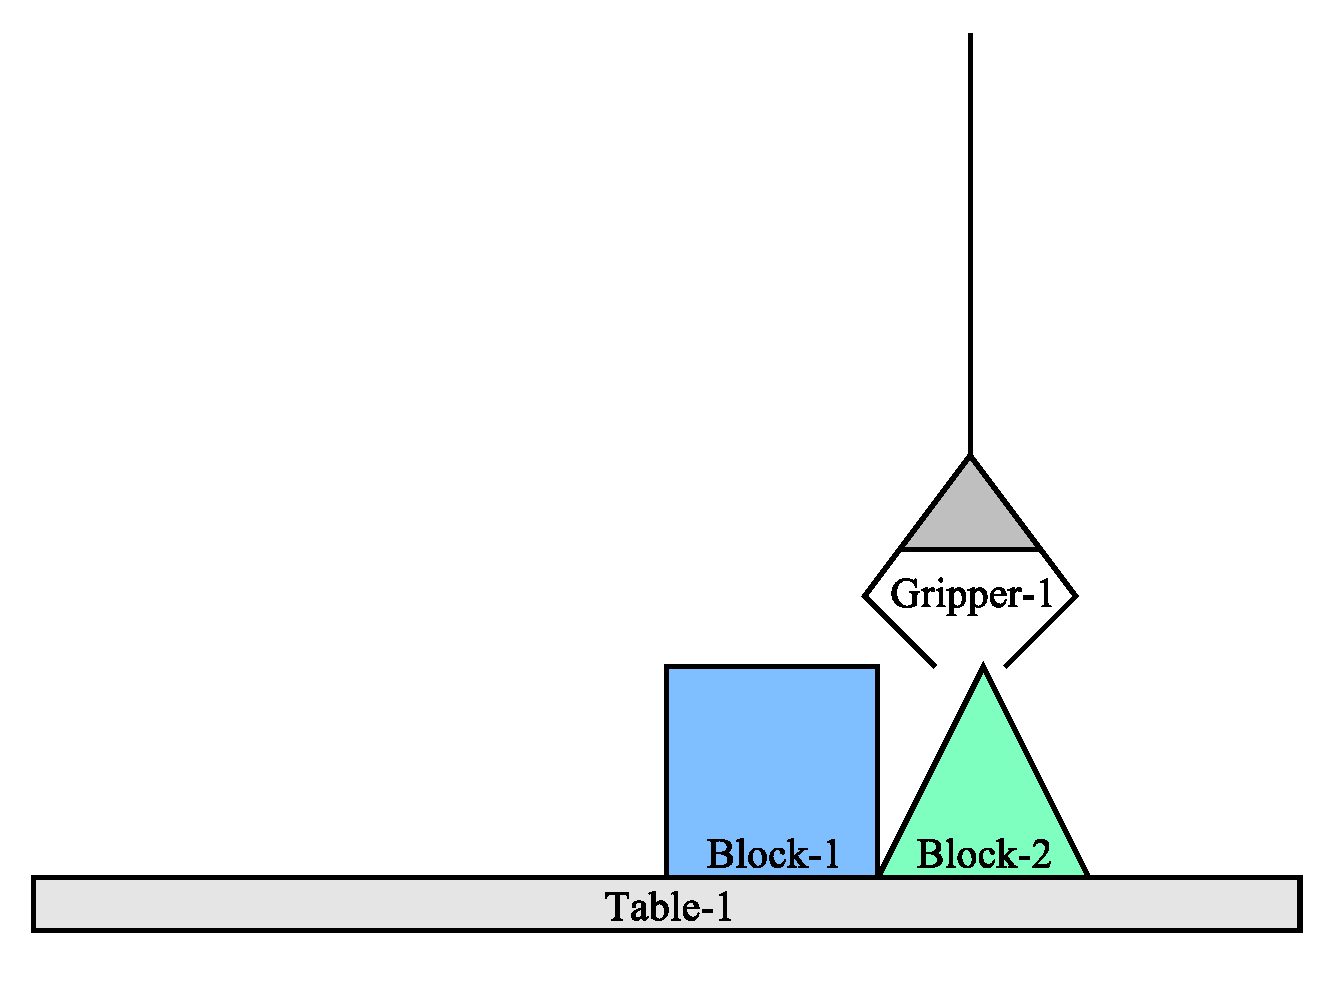
\includegraphics[width=3.5cm]{gfx/blocks_world_example-9} \\
%% 10. 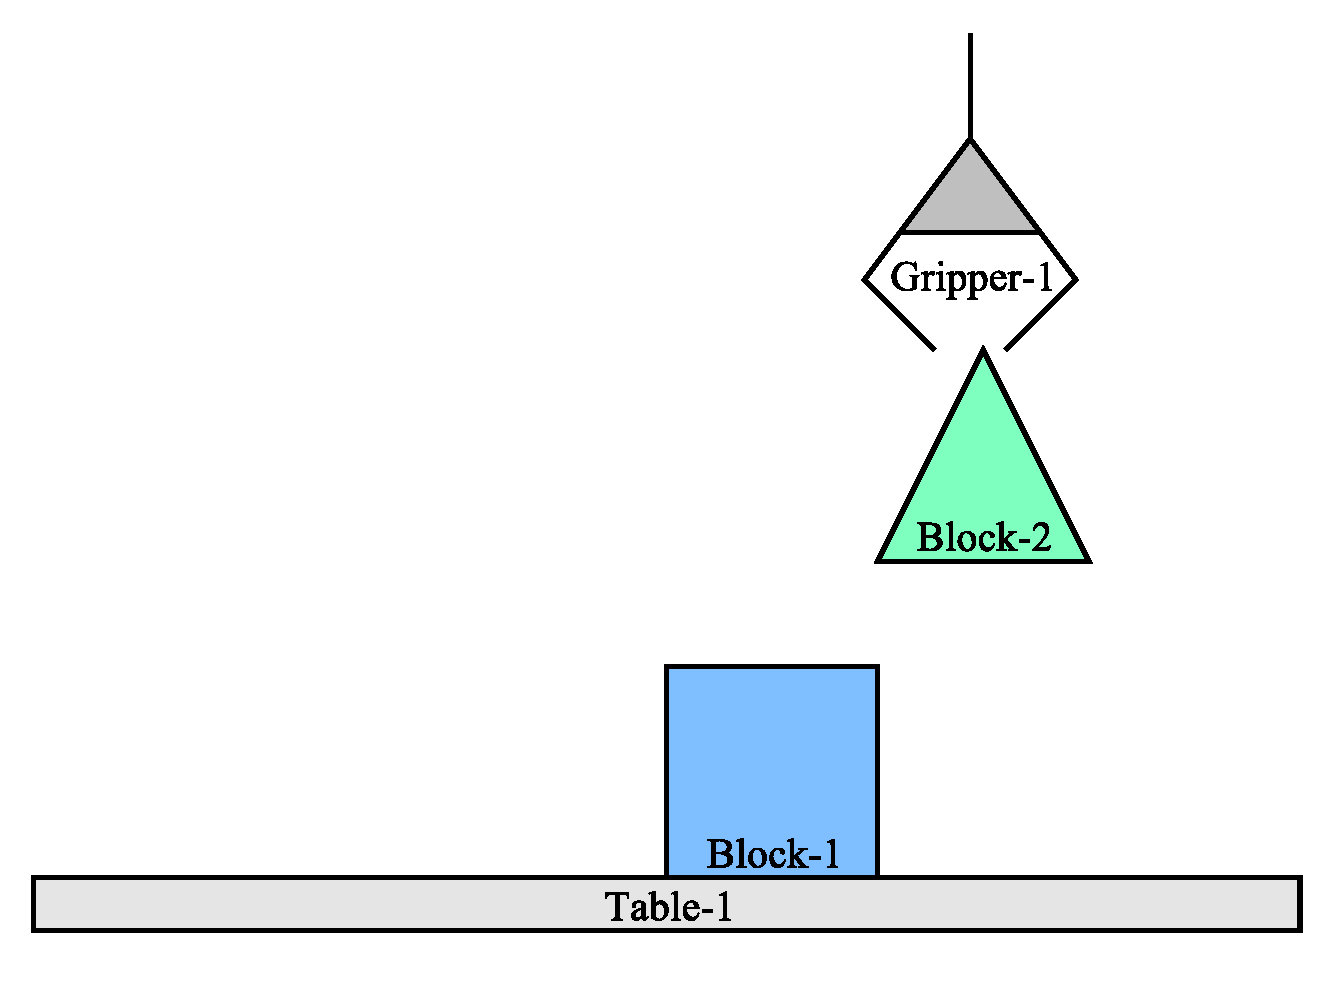
\includegraphics[width=3.5cm]{gfx/blocks_world_example-10} & 11. 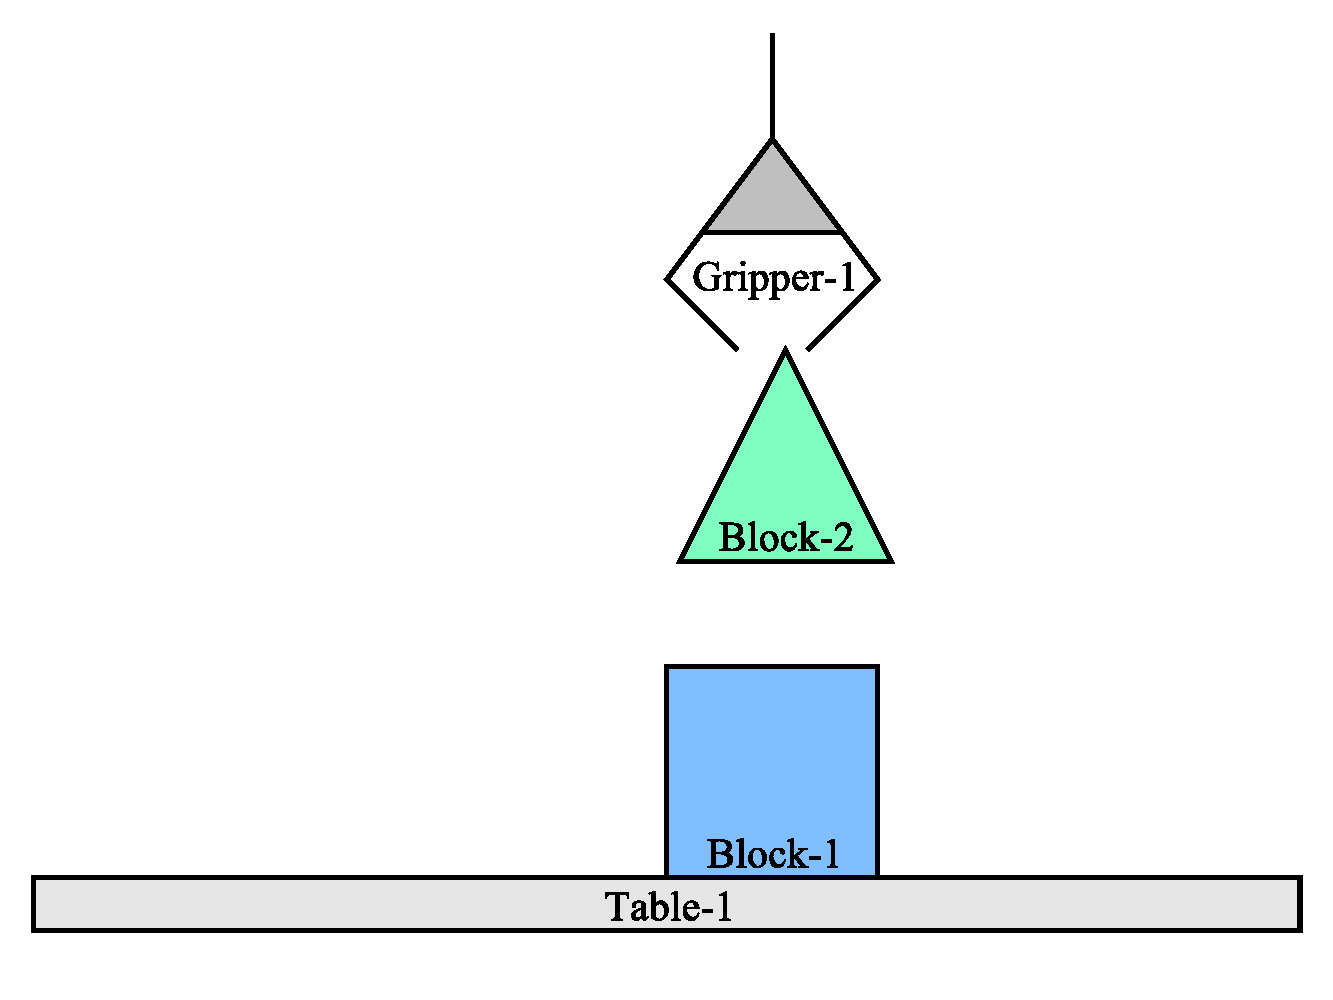
\includegraphics[width=3.5cm]{gfx/blocks_world_example-11} & 12. 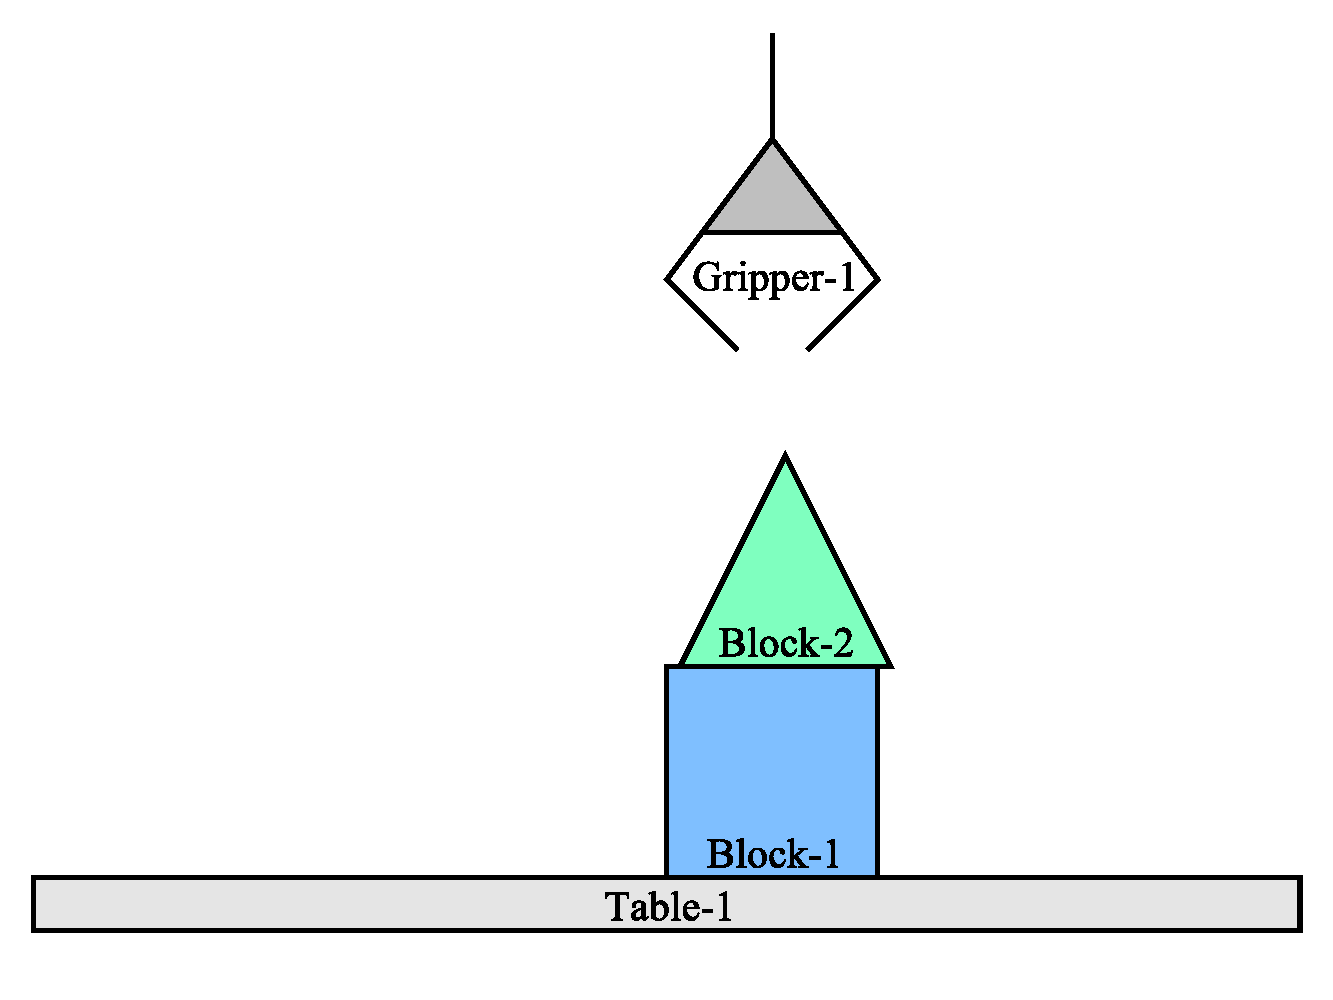
\includegraphics[width=3.5cm]{gfx/blocks_world_example-12}
%% \end{tabular}
%% \caption[Adaptation due to reflectively learning how to
%%   deliberate.]{Adaptation due to reflectively learning how to
%%   deliberate.  The AI has the goal of creating a stack of two blocks.
%%   (1) A plan is recalled from memory and executed because it asserts
%%   that a cube is sitting on a pyramid, which hypothetically
%%   accomplishes the goal.  (2--8) The deliberative layer executes the
%%   plan and because the cube falls off of the pyramid, the plan's
%%   assertion fails, an expectation failure that is reported to the
%%   reflective layer.  (8) The reflective layer hypothesizes that plans
%%   asserting a stack of a cube on a pyramid will lead to failure when
%%   executed.  The reflective layer selects a new planning strategy that
%%   it infers will not lead to failure: executing a plan from memory
%%   that is hypothesized to stack a pyramid on a cube.  (9-12) The
%%   second plan completes execution, successfully asserting that a
%%   pyramid is stacked on a cube.}
%% \label{figure:implemented_example_learning_storyboard}
%% \end{figure}

%% \section{The Four Layers of the AI}

%% The AI is a four-layered real-time reflective control system.  Each
%% layer is informed by receiving streams of events from the layers
%% below.  Also, each layer sends activation and suppression commands in
%% order to control the layers below.  This four-layered model is
%% inspired by the bottom four layers of the six-layered Emotion Machine
%% architecture for human commonsense thinking \cite[]{minsky:2006}.  The
%% four layers of the AI reflectively control a physical simulation.
%% {\mbox{\autoref{figure:four_layers_overview}}} shows an overview of
%% the four layers of the AI in relation to the physical simulation.
%% \begin{figure}
%% \begin{center}
%% 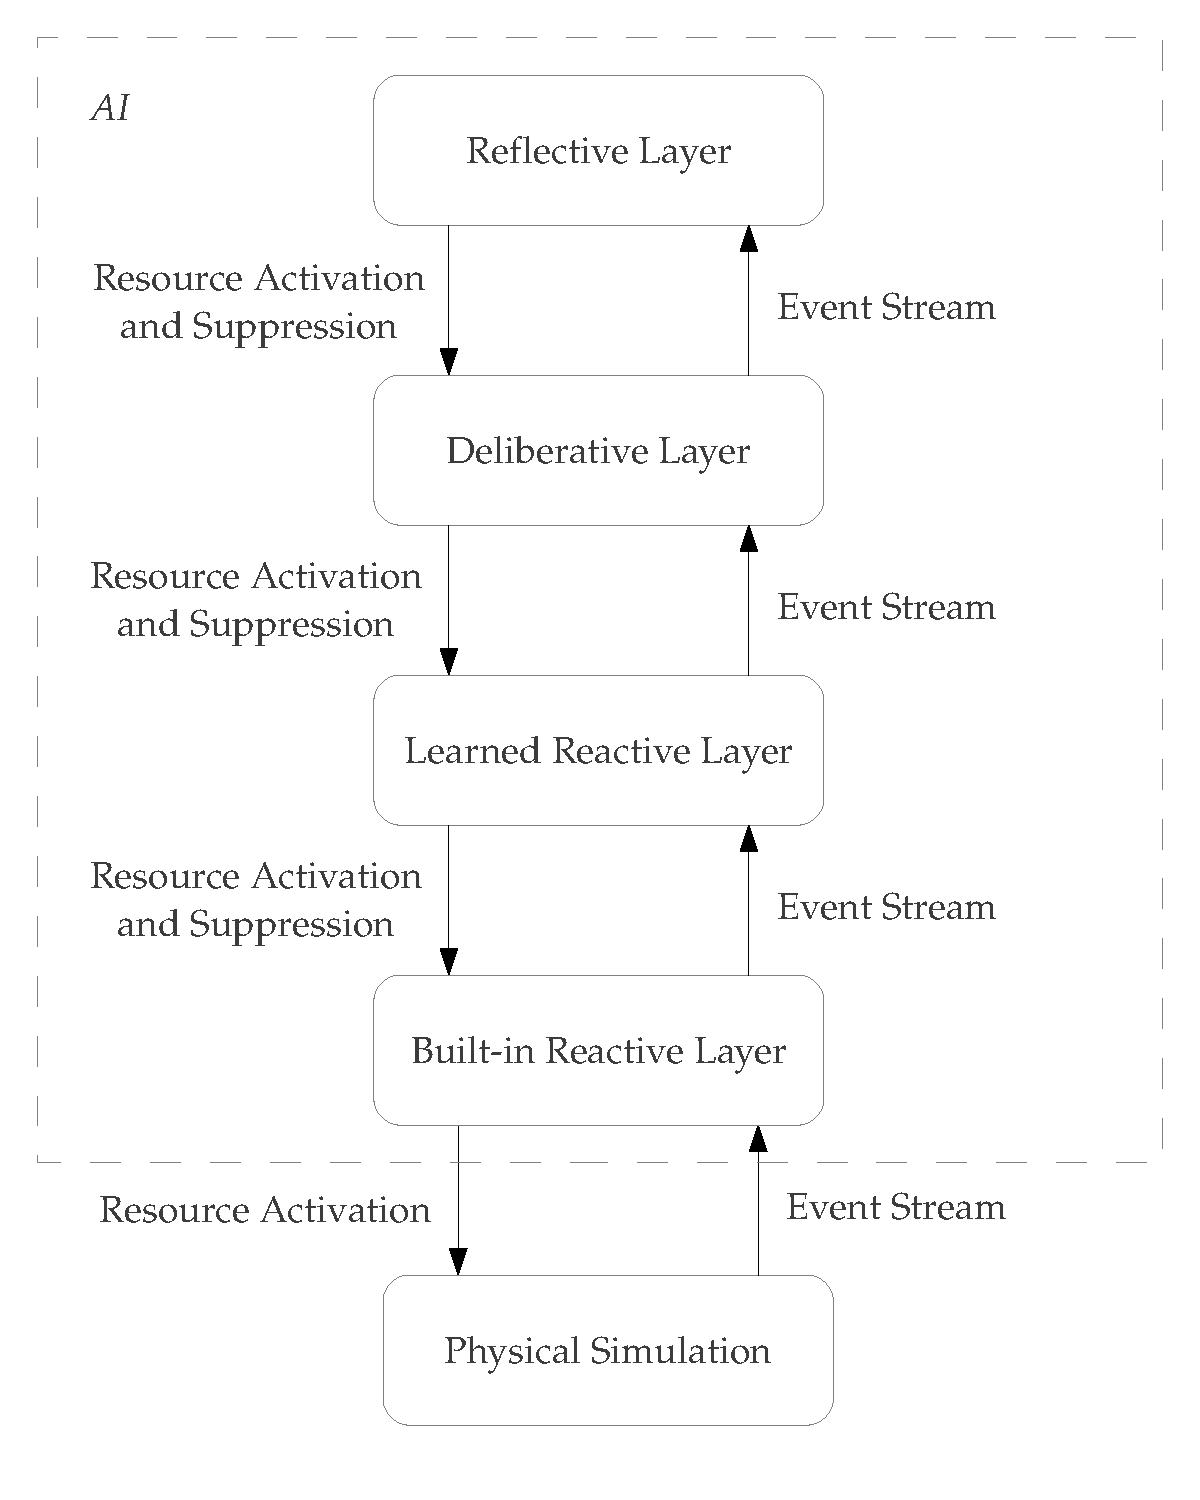
\includegraphics[width=10cm]{gfx/four_layers_overview}
%% \end{center}
%% \caption[The four layers of the AI in relation to the physical
%%   simulation.]{The layers of the AI in relation to the physical
%%   simulation.  The four layers of the AI form cascaded control loops,
%%   where each layer reflectively controls the layers below.}
%% \label{figure:four_layers_overview}
%% \end{figure}

%% In the following sections, I give an overview of the types of
%% knowledge and processes that comprise the physical simulation as well
%% as each of the four layers of reflective control in the AI that
%% simulate this example of reflectively learning not only to physically
%% act but also to deliberatively plan.  These following sections will
%% only be a cursory overview of the layers.  The AI is organized into
%% layers of reflection that are each themselves composed of
%% \emph{agencies} that are in turn composed of \emph{resources} that can
%% be controlled and executed concurrently by the layers above.

%% \section{The Physical Simulation}

%% The block building domain is implemented as a simulation based on
%% two-dimensional ridid-body physical laws, including floating point
%% numerical representations for object positions, velocities and
%% accelerations.  Changes in the semantic relationships between objects
%% in the physical simulation are sent in a stream of perceptual events
%% from the physical simulation to the AI.  The semantic relationships
%% that are computed by the physical simulation are basic visual
%% relationships, such as the prepositional relationships, ``$X$ is on
%% top of $Y$'' and ``$X$ is to the left of $Y$'', as well as visual
%% properties, such as ``$X$ is the color $Y$'' or ``$X$ has the shape
%% $Y$''.  This semantic visual knowledge is represented as frame-based
%% objects in the physical simulation, which reports any changes to this
%% knowledge to the AI as a stream of visual events.  For example, the
%% semantic knowledge can be thought of as a list of the following types
%% of subject-verb-object sentences:
%% \begin{itemize}
%% \item Block-1 is-a block.
%% \item Table-1 is-a table.
%% \item Gripper-1 is-a gripper.
%% \item Block-1 has-the-color blue.
%% \item Block-2 has-the-shape pyramid.
%% \item Block-1 is-on Table-1.
%% \item Block-2 is-on Table-1.
%% \item Gripper-1 is-holding Block-1.
%% \item Gripper-1 is-above Table-1.
%% \item Block-2 is-to-the-left-of Gripper-1.
%% \end{itemize}
%% The physical simulation generates a list of these simple
%% subject-verb-object sentences in its internal state.  The actual
%% internal lisp-like representation of the physical simulation is shown
%% in \autoref{table:internal_lisp_like_physical_representation}.
%% \begin{table}[h]
%% \begin{center}
%% {\fbox{
%% \begin{tabular}{l}
%%  {\tt{[Block-1 left-of Gripper-1]}} \\
%%  {\tt{[Block-1 on Table-1]}} \\
%%  {\tt{[Block-1 shape cube]}} \\
%%  {\tt{[Block-1 color blue]}} \\
%%  {\tt{[Block-1 is-a block]}} \\
%%  {\tt{[Block-2 right-of Gripper-1]}} \\
%%  {\tt{[Block-2 on Table-1]}} \\
%%  {\tt{[Block-2 shape pyramid]}} \\
%%  {\tt{[Block-2 color green]}} \\
%%  {\tt{[Block-2 is-a block]}} \\
%%  {\tt{[Table-1 left-of Gripper-1]}} \\
%%  {\tt{[Table-1 shape cube]}} \\
%%  {\tt{[Table-1 color white]}} \\
%%  {\tt{[Table-1 is-a table]}} \\
%%  {\tt{[Gripper-1 is-holding []]}} \\
%%  {\tt{[Gripper-1 color black]}} \\
%%  {\tt{[Gripper-1 is-a gripper]}} \\
%%  {\tt{[Gripper-1 movement\_command stop]}} \\
%%  {\tt{[Gripper-1 is me]}}
%% \end{tabular}
%% }}
%% \end{center}
%% \caption[Internal semantic visual representation generated by the body
%%   in the physical simulation.]{Internal semantic visual representation
%%   generated by the body in the physical simulation.  Changes to this
%%   representation are sent as a stream of visual change events to the
%%   built-in reactive layer of the AI.}
%% \label{table:internal_lisp_like_physical_representation}
%% \end{table}

%% \section{The Built-in Reactive Layer}

%% The physical simulation generates a stream of events that represent
%% changes in the perceptual state of the body of the AI.  The first
%% layer of the AI is \emph{the built-in reactive layer}, which monitors
%% this event stream of perceptual changes in object knowledge from the
%% physical simulation.  These changes in the perceptual state of the
%% AI's body in the physical simulation are reconstructed in the built-in
%% reactive layer.  In this way, the built-in reactive layer maintains a
%% representation of the visual knowledge that the body is currently
%% seeing.  The representation of the perceptual state of the body that
%% informs the AI about the physical world is referred to as \emph{the
%%   visual knowledge base}.  The built-in reactive layer also contains
%% predefined physical action resources that are available in the
%% physical body of the AI in the physical simulation.  Because the
%% built-in reactive layer is the primary interface to the physical body
%% that the AI controls, many of the resources of the built-in layer are
%% actually defined by the physical simulation during the initial boot-up
%% process of the entire AI-physical-simulation system.  Also, the
%% specific types of semantic visual objects and prepositional
%% relationships and properties are not known to the mind until they are
%% received from the physical simulation.  The AI simply expects to
%% receive a stream of visual objects, their relationships, and
%% properties.

%% \section{The Learned Reactive Layer}

%% Changes to the visual knowledge base in the built-in reactive layer
%% constitute the stream of events that \emph{the learned reactive layer}
%% receives and reconstructs into a more stable representation of the
%% physical world.  The AI's current representation of the physical world
%% is referred to as \emph{the physical knowledge base}.  I have found
%% the distinction between visual and physical knowledge to be useful in
%% domains where only partial information about the physical world is
%% available through the senses.  In this case, some reasoning must be
%% done in order to debug the physical knowledge when contradictory
%% visual input is detected.  For example, {\mbox{\cite{smith:2010}}}
%% describe a {\emph{kitchen cooking domain}}, shown in
%% {\mbox{\autoref{figure:isis_world_two_agents}}}.  In the kitchen
%% cooking domain, the AI sees a stick of butter in the refrigerator.
%% Subsequently, the AI sees the same stick of butter on a table.  The AI
%% must resolve the fact the either (1) the table is small enough to fit
%% into the refrigerator or (2) the stick of butter is no longer in the
%% refrigerator.  The reactive layers of the AI that are necessary for
%% navigating the kitchen domain are factors that complicate explaining
%% the deliberative and reflective thinking layers of the AI.  The
%% learning and planning agencies of the deliberative and reflective
%% thinking layers are exactly the same for the block building domain as
%% they are for the kitchen domain.  Thus, I will focus on explaining the
%% AI's reflective thinking processes in terms of the simpler block
%% building domain as the reflective thinking capabilities are the focus
%% of this thesis.  In the block building domain, the physical knowledge
%% base is a faithful reconstruction of the visual knowledge base,
%% slightly behind the times.
%% {\mbox{\autoref{figure:implemented_physical_knowledge}}} shows the
%% physical knowledge base that is reconstructed from the reflective
%% change events that the learned reactive layer receives from changes in
%% the visual knowledge base of the built-in reactive layer.
%% \begin{figure}
%% \begin{center}
%% 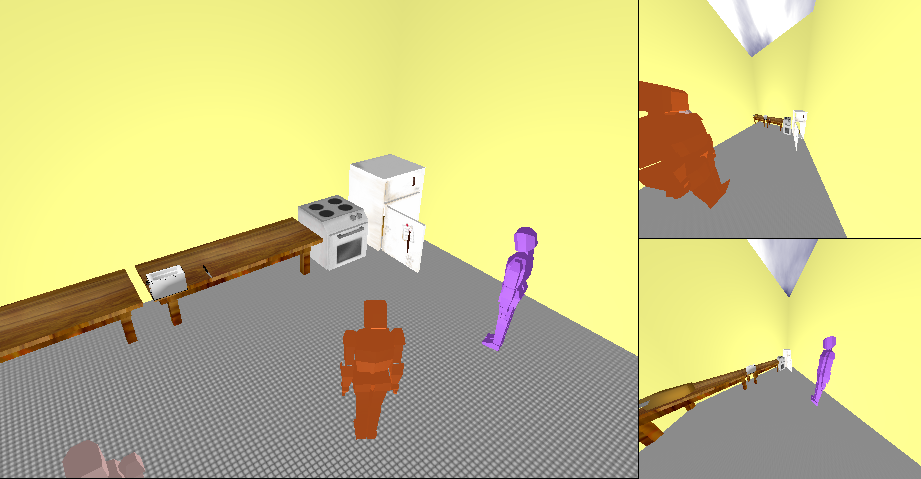
\includegraphics[width=12cm]{gfx/isis_world_two_agents}
%% \end{center}
%% \caption[Kitchen cooking domain with partial visual knowledge of the
%%   physical domain.]{Kitchen cooking domain with only partial visual
%%   knowledge of the physical domain available to the AI.  The image on
%%   the left is a bird's-eye-view of the situation, while the images on
%%   the right contain the objects that each AI can actually see.}
%% \label{figure:isis_world_two_agents}
%% \end{figure}
%% \begin{sidewaysfigure}
%% \begin{center}
%% 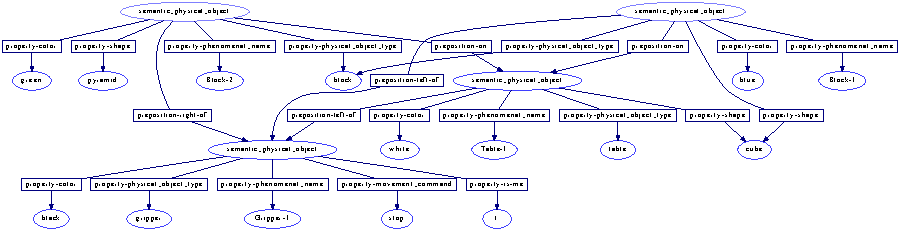
\includegraphics[width=8.5in]{gfx/implemented_physical_knowledge}
%% \end{center}
%% \hspace{4cm}\parbox{15cm}{\caption[The physical knowledge base.]{The
%%     physical
%%     knowledge base.}\label{figure:implemented_physical_knowledge}}
%% \end{sidewaysfigure}

%% \section{The Deliberative Layer}

%% \emph{The deliberative layer} receives a stream of events from the
%% learned reactive layer including changes to the physical knowledge
%% base as well as changes in the activation states of reactive
%% resources.  While the reactive layer may react to visual or physical
%% knowledge immediately, the deliberative layer learns models of this
%% reactive behavior at a more steady and often slower pace.  This allows
%% the reactive layer to operate at full speed, often in bursts of
%% activity, while a buffered stream of events is reasoned about more
%% carefully by the deliberative layer without slowing the primary
%% activity of physical reaction.  The deliberative layer first
%% reconstructs a copy of the physical knowledge base that it can use as
%% reference for the slower deliberative learning processes.  From this
%% reconstruction of the physical knowledge base, the deliberative layer
%% induces and counts common types of knowledge.  This type induction
%% process is focused only on the parts of the physical knowledge base
%% that have changed.  The deliberative layer stores counts of these
%% types of knowledge in a knowledge base in the deliberative layer
%% called \emph{the physical type knowledge base}.  The physical type
%% knowledge base counts the occurrences of types of knowledge in the
%% deliberative layer's reconstruction of the physical knowledge base.
%% {\mbox{\autoref{figure:physical_type_knowledge_induction}}} shows the
%% knowledge bases involved in the induction of physical type knowledge.
%% The following is a list of types of physical type knowledge that is
%% accounted for in the physical type knowledge base at any given point
%% in time:
%% \begin{itemize}
%% \item A block is sitting on another block.
%% \item A block with a pyramid shape is sitting on Block-1.
%% \item A green block is sitting on a blue block.
%% \item A block is to the left of a gripper.
%% \end{itemize}
%% \begin{figure}
%% \begin{center}
%% 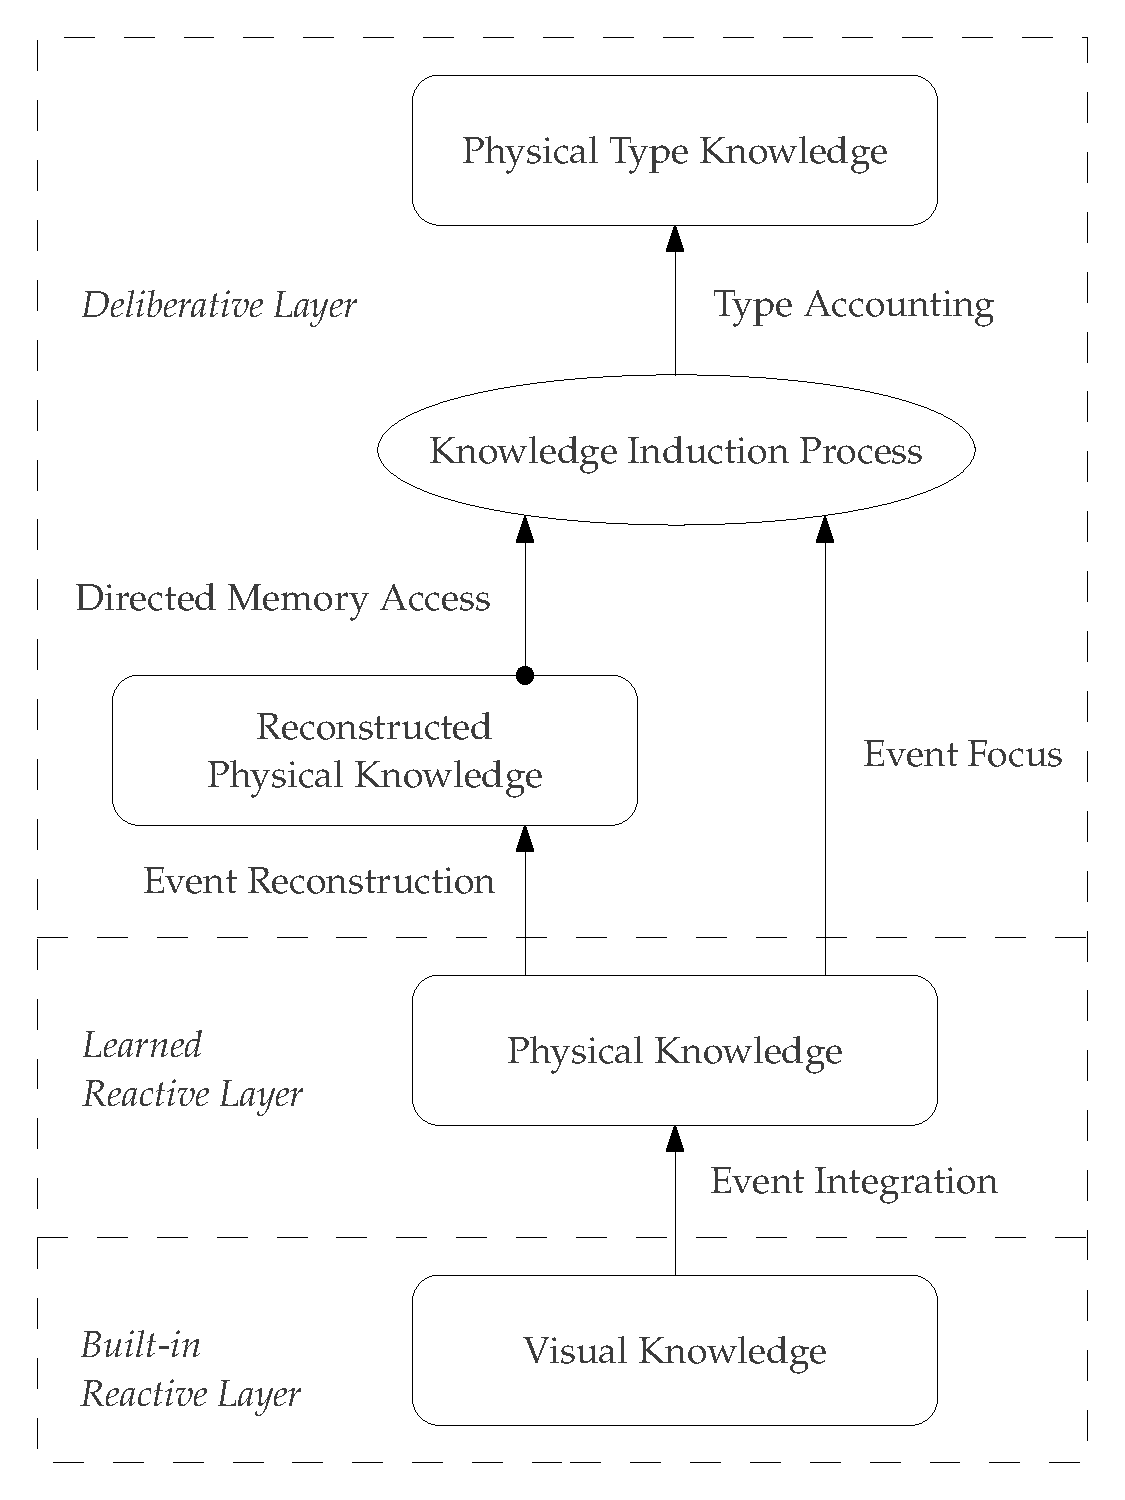
\includegraphics[width=10cm]{gfx/physical_type_knowledge_induction}
%% \end{center}
%% \caption[The knowledge bases involved in physical type knowledge
%%   induction.]{The knowledge bases involved in physical type knowledge
%%   induction.  The creation of a reconstruction of the physical
%%   knowledge base by the deliberative layer allows the full speed
%%   concurrent execution of the reactive layer, despite the slower speed
%%   of the more careful deliberative learning processes.}
%% \label{figure:physical_type_knowledge_induction}
%% \end{figure}

%% In addition to events about knowledge in the physical knowledge base
%% of the reactive layer, the deliberative layer also receives events
%% that specify the beginning and ending times of reactive layer resource
%% executions.  Resource execution events are causally traced, so that
%% execution call graphs are easily reconstructed asynchronously by the
%% deliberative layer.
%% {\mbox{\autoref{figure:implemented_reflective_event_knowledge_base}}}
%% shows a time-line visualization of the reflective event knowledge base
%% that is constructed from the execution events of the reactive
%% resources.  Once a beginning and an ending time for an execution event
%% in the reactive layer is received by the deliberative layer, a future
%% task is created to learn the physical type knowledge transframe for
%% this resource execution.  The learning of a physical type knowledge
%% transframe for the execution of a reactive resource must wait for the
%% physical type knowledge base to catch up with processing the current
%% information from the visual and physical knowledge bases in the
%% reactive layer.
%% \begin{figure}
%% \begin{center}
%% 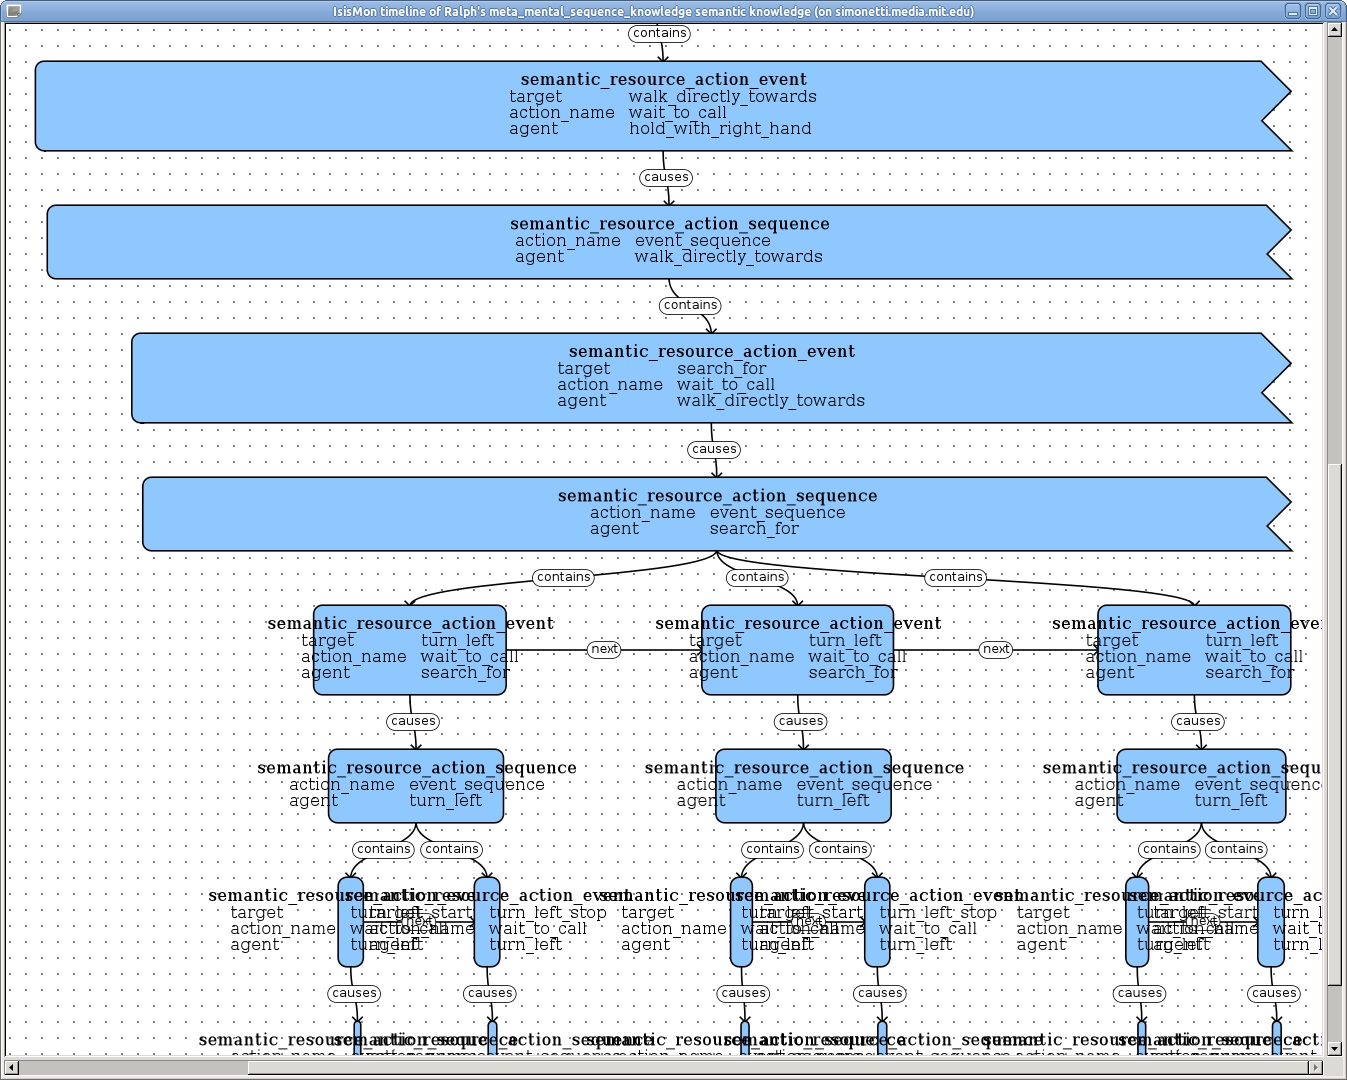
\includegraphics[width=10cm]{gfx/implemented_reflective_event_knowledge_base}
%% \end{center}
%% \caption[A time-line visualization of the reflective event knowledge
%%   base that is constructed from the execution events from the reactive
%%   resources.]{A time-line visualization of the reflective event
%%   knowledge base that is constructed from the execution events from
%%   the reactive resources has a hierarchical causal structure.  The
%%   horizontal axis represents time, while rounded rectangles represent
%%   execution events of different reactive resources.  Notice that some
%%   rectangles have a jagged right edge.  This represents that the event
%%   does not yet have an ending time.  Once an event has both a
%%   beginning and an ending time in this knowledge base, which a
%%   reflective process recognizes, the action transframe hypotheses are
%%   refined, given the new physical change correlations for the resource
%%   execution.  These physical change correlations are computed by an
%%   asynchronous process, so a new parallel learning task is created to
%%   wait for this event.}
%% \label{figure:implemented_reflective_event_knowledge_base}
%% \end{figure}

%% Once a physical type transframe is computed for a reactive event, a
%% version space concept learning algorithm \cite[]{mitchell:1997} is
%% created for each add or remove physical type knowledge change in the
%% transframe.  In the concept learning algorithm, a conjunctive
%% hypothesis space of predictive physical type preconditions is
%% represented in terms of a version space generalization lattice, so
%% that all possibly correct hypotheses that predict the transframe
%% change evidence are represented in a relatively compact way.  Once a
%% hypothesis space is created for a transframe change, this hypothesis
%% space is associated with the reactive action so that it may be used by
%% the deliberative layer to infer the counterfactual results of
%% executing the action in its planning machine.
%% {\mbox{\autoref{table:abstract_physical_transframe}}} shows an example
%% of a physical type knowledge transframe based on the changes in the
%% physical type knowledge base over time.
%% \begin{table}[h]
%% \centering
%% \begin{tabular}{c}
%%   Hypothesized Physical Type Knowledge Transframe for Action \\
%%   \begin{tabular}{|l|l|}
%%     \hline
%%     \emph{action:}        & Reach and grab. \\
%%     \hline
%%     \emph{preconditions:} & A block is below a gripper. \\
%%     ~                     & A gripper is holding nothing. \\
%%     \hline
%%     \emph{additions:}     & A gripper is holding a block. \\
%%     \hline
%%     \emph{removals:}      & A gripper is holding nothing. \\
%%     \hline
%%   \end{tabular}
%% \end{tabular}
%% \caption[Hypothesized physical type knowledge transframe for
%%   action.]{Hypothesized physical type knowledge transframe including
%%   action dependent sets of physical type knowledge \emph{add} and
%%   \emph{remove} changes with learned conjunctive hypothesis spaces
%%   based on a set of physical type knowledge preconditions.}
%% \label{table:abstract_physical_transframe}
%% \end{table}

%% In order to learn transframes from physical type knowledge, it is
%% useful to have the physical type knowledge base able to be indexed at
%% arbitrary points in the past.  This is achieved by representing
%% physical type knowledge in the form of events that have beginning and
%% ending times.  All events in the physical type knowledge base are
%% automatically organized into an interval tree, so that any temporal
%% indexing of the physical type knowledge base can be done with $O(\log
%% n)$ time complexity as $n$ increases linearly with the number of
%% physical type knowledge events in the knowledge base.  Thus, computing
%% the physical type knowledge transframe between any two points in the
%% past can be done relatively quickly.  A necessary feature that must
%% still be added to the architecture is a \emph{forgetful} physical type
%% knowledge base.  There are many forgetful event streams in the
%% language, and the ability to treat an entire event knowledge base as a
%% forgetful streaming object is a way to allow this knowledge base to
%% not grown indefinitely over the run-time of the algorithm.

%% Once the deliberative layer learns action dependent transframe
%% hypotheses in terms of the physical type knowledge, these hypotheses
%% can be used for imagining the hypothetical types of effects of
%% actions.  This hypothetically supported knowledge is stored by the
%% deliberative layer in \emph{the counterfactual physical type knowledge
%%   base}.  The counterfactual physical type knowledge is used for
%% imagining the execution of plans, a step in the planning process.
%% Plans sometimes assert conditions in the physical type knowledge base.
%% During the imagination of the plan execution, the counterfactual
%% physical type knowledge is used for determining whether assertions
%% will succeed or fail in the imagination of the plan's counterfactual
%% execution knowledge.  For example,
%% {\mbox{\autoref{table:a_plan_learned_from_being_told}}} on
%% {\mbox{page~\pageref{table:a_plan_learned_from_being_told}}} shows a
%% plan that contains the assertion that ``a cube is sitting on a
%% pyramid''.  The AI has no experience executing this plan because it
%% has only ``been told'' this plan.  The AI adds the types of knowledge
%% asserted within the plan to the possible hypothetical transframes for
%% the actions in the plan.  This causes the AI to have a concept learner
%% for predicting the change that would satisfy the assertion in the
%% plan.  Inferred counterfactual physical type knowledge can predict
%% both that an action in the plan will cause the knowledge necessary for
%% the assertion to succeed as well as that the knowledge for the
%% assertion will not be caused and the assertion will fail.  Notice that
%% even if a plan fails given certain preconditions, there is always the
%% potential that this plan will successfully complete under some
%% possible future preconditions.  The utility of the plan is learned
%% through experiences in different physical type preconditions.  In this
%% way, the inferred hypothetical effects of an action can be learned
%% from ``being told'' as well as eliminated through experience executing
%% the plan.

%% Finally, the deliberative layer goes through a list of the plans that
%% it knows and imagines executing them.  If the imagined plan succeeds
%% and accomplishes the physical type goals of the deliberative planning
%% machine, then the plan is executed.  The deliberative planning machine
%% has the following goal: ``A block is sitting on a block.''  When the
%% AI imagines executing the plan in
%% {\mbox{\autoref{table:a_plan_learned_from_being_told}}} on
%% {\mbox{page~\pageref{table:a_plan_learned_from_being_told}}}, there is
%% hypothetical support for the counterfactual knowledge: ``A cube is
%% sitting on a pyramid.''  The deliberative imagination agency infers
%% the hypothetical effects of the plan.  The counterfactual physical
%% type knowledge base contains the assertion of the plan, an instance of
%% the current physical type goal, ``A block is sitting on a block.''
%% Since the goal is hypothetically supported, the plan is executed by
%% the deliberative execution agency.  The experienced gained from
%% actually executing the plan results in the learning of a more refined
%% model of the physical world as well as a more refined model of the
%% deliberative planning machine.  The details of how the deliberative
%% infers hypothetically supported counterfactual knowledge so that it
%% can be corrected as hypotheses are refined in the learning process is
%% described in detail in the next chapter,
%% \autoref{chapter:grounded_learning_of_knowledge_utility},
%% ``\nameref{chapter:grounded_learning_of_knowledge_utility}.''

%% \section{The Reflective Layer}

%% While the deliberative layer learns hypothetical models of how
%% physical actions affect the types of physical knowledge, the
%% reflective layer learns hypothetical models of how deliberative
%% actions affect the types of deliberative knowledge.  The reflective
%% layer receives a stream of deliberative planning machine knowledge
%% events, which it uses to reconstruct a copy of the deliberative
%% planning machine knowledge base that it can use for inducing
%% deliberative type knowledge at a steadier pace than the shorter-lived
%% ``bursty'' executions of the deliberative planning machine resources.
%% The deliberative planning machine knowledge base does not contain
%% physical objects but instead contains deliberative objects, such as
%% the planning machine, goals, plans, and failure events.
%% {\mbox{\autoref{figure:deliberative_planning_machine_knowledge_base}}}
%% shows the deliberative planning machine knowledge base that the
%% reflective layer concurrently reconstructs from a procedural events
%% stream and learns hypotheses for how to control by imagining plans
%% involving the deliberative planning resources.
%% \begin{sidewaysfigure}
%%   \begin{tabular}{p{8in}}
%%     % define source coordinates
%%     \begin{itemize}
%%     \item Plan for Physical Action in Deliberative Planning Machine Focus Register \tikz[na] \coordinate (executing-plan-label);
%%     \item Plan for Physical Action in Deliberative Planning Machine Execute Register \tikz[na] \coordinate (focus-plan-label);
%%     \item Deliberative Planning Machine \tikz[na] \coordinate (deliberative-planning-machine-label);
%%     \end{itemize} \\
%%     % Use a background grid to make it easier to find coordinates
%%     % When the coordinates have been found, remove the 
%%     % 'show background grid' option. 
%%     %\tikzstyle{background grid}=[draw, black!50,step=.5cm]
%%     \begin{tikzpicture}%[show background grid]
%%       % Put the graphic inside a node. This makes it easy to place the
%%       % graphic and to draw on top of it. 
%%       % The above right option is used to place the lower left corner
%%       % of the image at the (0,0) coordinate. 
      
%%       \node [inner sep=0pt,above right] {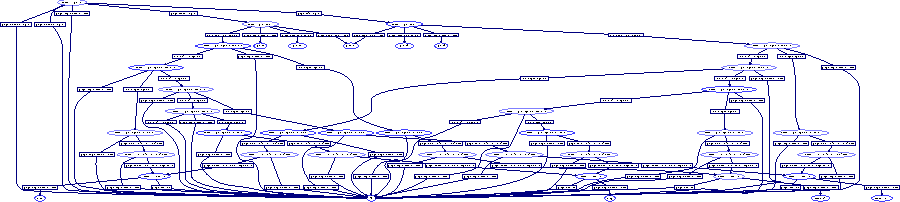
\includegraphics[width=8in]{gfx/deliberative_planning_machine_knowledge_base}};
      
%%       % show origin
%%       %\fill (0,0) circle (2pt);
%%       % define destination coordinates
%%       \path (17.5,2) coordinate (executing-plan)
%%       (6,2.25) coordinate (focus-plan)
%%       (1.75,4.5) coordinate (deliberative-planning-machine);
%%     \end{tikzpicture}
%%   \end{tabular}
  
%%   % define overlays
%%   % Note the use of the overlay option. This is required when 
%%   % you want to access nodes in different pictures.
%%   \begin{tikzpicture}[overlay]
%%     \draw (executing-plan) node[ellipse, dashed, dash pattern=on 10pt off 10pt, red, minimum height=4cm,minimum width=6cm, line width=1.5, draw] {};
%%     \path[->,red,thick, line width=1.5] (executing-plan-label) edge [out=0, in=120] (executing-plan);
    
%%     \draw (focus-plan) node[ellipse, dashed, dash pattern=on 10pt off 10pt, red, minimum height=4cm,minimum width=6cm, line width=1.5, draw] {};
%%     \path[->,red,thick, line width=1.5] (focus-plan-label) edge [out=0, in=60] (focus-plan);
    
%%     \draw (deliberative-planning-machine) node[ellipse, dashed, dash pattern=on 10pt off 10pt, red, minimum height=0.5cm,minimum width=1.5cm, line width=1.5, draw] {};
%%     \path[->,red,thick, line width=1.5] (deliberative-planning-machine-label) edge [out=0, in=-60] (deliberative-planning-machine);
%%   \end{tikzpicture}
%%   \hspace{4cm}\parbox{15cm}{\caption[The deliberative planning machine
%%       knowledge base with the deliberative planning machine and two
%%       plans.]{The deliberative planning machine knowledge base with
%%       the deliberative planning machine and two plans are circled.
%%       These plans are each on one of the planning machine's registers,
%%       the \emph{focus} register and the \emph{execution}
%%       register.}\label{figure:deliberative_planning_machine_knowledge_base}}
%% \end{sidewaysfigure}

%% The reflective layer learns to make plans for accomplishing and
%% avoiding types of deliberative knowledge states.  Analagously to how
%% physical type knowledge is induced from the specific physical states,
%% the reflective layer induces types of deliberative planning machine
%% knowledge from the specific deliberative planning machine states.  If
%% a specific planning machine state is ``Plan-1 is in
%% Planning-Machine-1's focus register and has had the failure
%% Expectation-Failure-1,'' the following type knowledge can be induced
%% from this specific state: ``A plan is in a planning machine's focus
%% register,'' and ``A plan has had a failure.''
%% {\mbox{\autoref{figure:deliberative_type_knowledge_induction}}} shows
%% an overview of the knowledge bases and processes involved in the
%% induction of the deliberative planning machine type knowledge base
%% from the deliberative planning machine knowledge base by the
%% reflective layer.  The reflective layer uses an analogous type
%% knowledge induction process as the deliberative layer, previously
%% shown in {\mbox{\autoref{figure:physical_type_knowledge_induction}}}
%% on {\mbox{page~\pageref{figure:physical_type_knowledge_induction}}}.
%% \begin{figure}[h]
%% \centering
%% 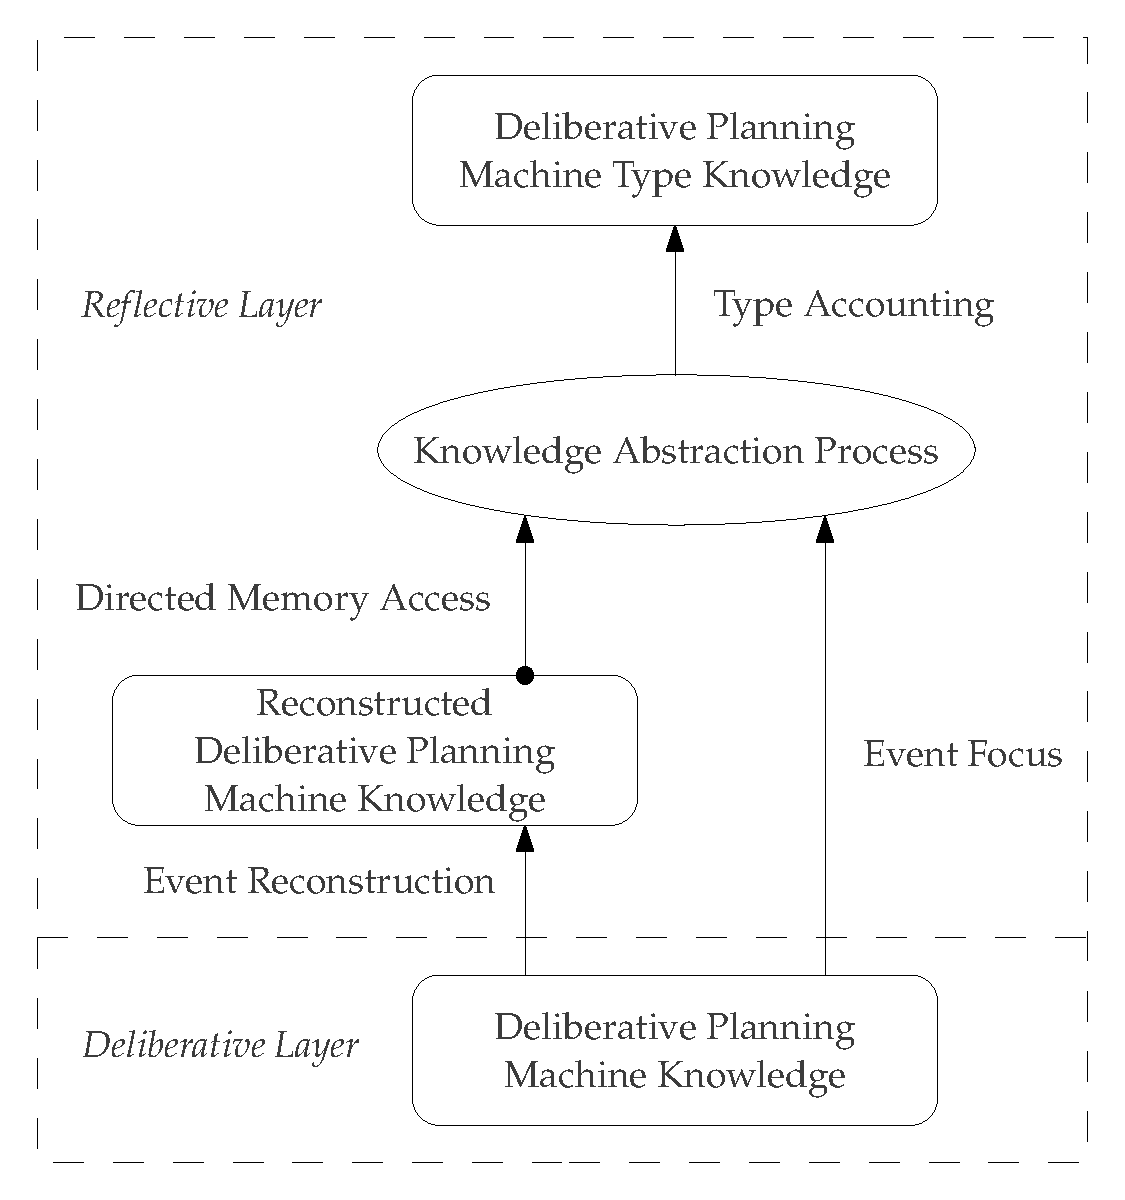
\includegraphics[width=10cm]{gfx/deliberative_type_knowledge_induction}
%% \caption[The knowledge bases and processes involved in deliberative
%%   planning machine type knowledge induction.]{The knowledge bases and
%%   processes involved in deliberative planning machine type knowledge
%%   induction.  The creation of a reconstruction of the deliberative
%%   planning machine knowledge base by the reflective layer allows the
%%   full speed concurrent execution of the deliberative planning
%%   machine, despite the slower speed of the more careful reflective
%%   learning processes.}
%% \label{figure:deliberative_type_knowledge_induction}
%% \end{figure}

%% Plans in the reflective planning machine knowledge base are imagined
%% in terms of the deliberative type knowledge.  This allows the
%% reflective layer planning machine to learn models of plan execution
%% that have no physical simulation component.  The ability to imagine
%% executing a plan and predicting its failure based on the structure of
%% the plan in relation to the planning machine and not in terms of the
%% physical world, is \emph{not} an advantage provided by physical
%% knowledge induction.  In this case, the ability to reason abstractly
%% about physical plans for action without any physical simulation
%% component necessary is provided by the reflective planning machine in
%% the reflective layer.  Hypotheses are learned by the reflective layer
%% that predict plan failure due to conjunctions of deliberative type
%% knowledge features.  One of the hypothetical deliberative type
%% knowledge transframes that the AI learns is the example expectation
%% failure is shown in
%% {\mbox{\autoref{table:hypothesized_deliberative_transframe}}}.
%% \begin{table}[h]
%% \centering
%% \begin{tabular}{c}
%%   Hypothesized Deliberative Type Knowledge Transframe for Action \\
%%   \begin{tabular}{|l|p{8cm}|}
%%     \hline
%%     \emph{action:}        & Execute and wait to complete. \\
%%     \hline
%%     \emph{preconditions:} & A plan is in focus that asserts a cube is sitting on a pyramid. \\
%%     ~                     & No plans have failed. \\
%%     \hline
%%     \emph{additions:}     & A plan has that just encountered a failure encountered an expectation failure. \\
%%     \hline
%%     \emph{removals:}      & No plans have failed. \\
%%     \hline
%%   \end{tabular}
%% \end{tabular}
%% \caption[Hypothesized deliberative type knowledge transframe for
%%   action.]{Hypothesized deliberative type knowledge transframe
%%   including action dependent sets of deliberative type knowledge
%%   \emph{add} and \emph{remove} changes with learned conjunctive
%%   hypothesis spaces based on a set of deliberative type knowledge
%%   preconditions.}
%% \label{table:hypothesized_deliberative_transframe}
%% \end{table}

%% The details of how the deliberative and reflective layers infer
%% hypothetically supported counterfactual knowledge so that it can be
%% corrected as hypotheses are refined in the learning process is
%% described in terms of detailed examples in the next chapter,
%% \autoref{chapter:grounded_learning_of_knowledge_utility},
%% ``\nameref{chapter:grounded_learning_of_knowledge_utility}.''



%% \newpage
%% \section{very old stuff from last chapter}

%% The Emotion Machine cognitive architecture that has been implemented
%% in this thesis exists as sets of concurrent problem solving
%% \emph{resources} that can activated or suppressed in order to
%% implement different \emph{ways of thinking}, configurations of
%% resources that are good for solving specific types of problems.  The
%% following are examples of physical action resources that could be
%% built into the physical simulation that the architecture is attempting
%% to control into being in specific goal configurations:
%% \begin{itemize}
%% \item \emph{Move left}
%% \item \emph{Move right}
%% \item \emph{Reach}
%% \item \emph{Grab}
%% \item \emph{Stop}
%% \item \emph{Drop}
%% \end{itemize}


%% Similar groups of resources that work together on a specific problem
%% domain are grouped into \emph{agencies}.

%% that can four reflective
%% layers that learn to control a physical simulation in order to
%% accomplish physical goals.  Also, because the algorithm is reflective
%% and can reason about its own reasoning processes, it is capable of
%% learning to accomplish reasoning goals, such as avoiding creating and
%% executing plans that fail.  These two layers of reasoners are
%% implemented in the top two reflective layers of the architecture.  The
%% cognitive architecture consists of four layers in total:
%% \begin{enumerate}
%% \item \emph{Built-in Reactive}: Contains basic representations for the
%%   primitive actions and perceptions provided by the physical
%%   simulation.
%% \item \emph{Learned Reactive}: Contains compiled plans that reference
%%   built-in reactive resources.
%% \item \emph{Deliberative}: Contains representations for the actions
%%   and reflective perceptions provided by the deliberative planning
%%   machine.
%% \item \emph{Reflective}: Contains representations for the actions of
%%   the reflective planning of new plans for deliberation.
%% \end{enumerate}


%% \section{SALS Controllable Object and Planning Layer Intro}

%% SALS includes the software implementation of two basic software
%% objects: (1) a controllable object, and (2) a planning layer object.
%% The controllable object includes a knowledge base, which can represent
%% a control domain, such as the physical knowledge signified by the
%% image in {\autoref{figure:introduction_example_problem_domain}}.
%% The planning layer object is a goal-oriented planning machine that
%% learns, creates, imagines, and executes plans in order to attempt to
%% control a given controllable object.  SALS becomes reflective because
%% the SALS planning layer object is also a controllable object, which
%% allows creating a linked list of planning layer objects all deriving
%% from a single original controllable object.  The form of this
%% reflective linked list structure implies a lot about the resulting
%% SALS cognitive architecture, and I will return to this idea often
%% throughout the dissertation.



%% \newpage
%% \section{Old Beginning of this chapter}

%% Hypothetical type knowledge transframes are used by the deliberative
%% and reflective planning machines in order to infer the effects of
%% executing plans.  There is a distinction here made between the
%% \emph{factual} knowledge that is directly an abstraction of knowledge
%% grounded in the physical or deliberative planning machine knowledge
%% bases, which are not based on any learned action hypotheses, and the
%% \emph{counterfactual} knowledge that is inferred and supported by
%% hypotheses of the effects of resource executions that the AI has
%% either ``been told'' or has learned in the course of actually
%% executing those resources in different contexts.  In order to maintain
%% this distinction in the AI, different knowledge bases are used to
%% separate the factual knowledge from counterfactual knowledge.  Factual
%% knowledge is induced into factual type knowledge abstractions.  The
%% factually grounded knowledge bases include the visual, physical,
%% physical type, deliberative planning machine, and deliberative
%% planning machine type knowledge bases.  However, the addition of
%% factually grounded knowledge causes a loss of hypotheses from the
%% resource execution type knowledge transframe hypothesis spaces in both
%% the deliberative and reflective layers.  Each counterfactual event in
%% the counterfactual knowledge bases has a list of dependencies that
%% must maintain their support in order for the counterfactual knowledge
%% to continue to exist.  Dependencies in the AI have three types of
%% support that can be rearranged in order to maintain the support of
%% counterfactual knowledge events:
%% \begin{enumerate}
%% \item Resource execution transframe preconditions.
%% \item Resource execution.
%% \item Resource execution transframe change hypotheses.
%% \end{enumerate}
%% If any of these three types of supports loses its hypothetical factual
%% grounding, this loss of hypothetical factual grounding causes the
%% dependency to become \emph{invalidated}.  Once a dependency has become
%% invalidated, it has a chance to find new hypothetical grounding before
%% it becomes \emph{unsupported}.  Counterfactual event knowledge is
%% notified when a dependency has become unsupported, causing the
%% counterfactual events to be removed from the counterfactual event
%% knowledge bases.  Also, as some counterfactual knowledge may form
%% hypothetical grounding for further dependencies of further
%% counterfactual event knowledge, the loss of support for a dependency
%% can cause a chain reaction through events and the dependencies that
%% rely on these events for grounding.  In this way, additional factual
%% knowledge refines and reduces the hypothetical support of transframe
%% changes, invalidating hypothetical dependencies, and potentially
%% causing the loss of support for counterfactual knowledge that has been
%% inferred in the counterfactual event knowledge bases of the
%% deliberative and reflective layers of the AI.

%% \section{Learning from Being Told Deliberative Plans}

%% In {\mbox{\autoref{table:a_plan_learned_from_being_told}}} on page
%% {\mbox{\pageref{table:a_plan_learned_from_being_told}}}, there is an
%% assertion at the end of the plan for reactive resource execution that
%% the AI has been told: ``Assert a cube is sitting on a pyramid.''  When
%% the AI initially learns a plan from being told, it does not yet have
%% any factual knowledge to eliminate any hypotheses about the effects of
%% the resource executions.  When the AI learns plan knowledge from being
%% told, the asserted type knowledge in the plan are added to the
%% resource execution hypothesis spaces before the assertion.  In this
%% case, the resource execution immediately before the assertion is:
%% ``Drop and wait for block to fall.''  Therefore, the AI does not
%% eliminate any hypotheses from the resource execution hypothesis spaces
%% but instead augments the potential \emph{change features} of this
%% resource's hypothesis spaces with this new \emph{add} change.  In
%% other words, the hypothesis space for the resource execution is
%% augmented to include all consistent hypotheses that both predict this
%% change and that do not predict this change.  Since the AI has no
%% previous factual knowledge about this change, it is capable of
%% predicting both possibilities, each with different sets of supporting
%% hypotheses: (1) that this feature is added when the resource is
%% executed in the given preconditions or (2) that this feature is not
%% added in the given preconditions.
%% {\mbox{\autoref{figure:inference_of_physical_knowledge}}} shows how
%% the augmented hypothesis space of this resource execution causes the
%% imaginative inference that will result in the future counterfactual
%% knowledge: ``A cube is sitting on a pyramid.''  Also, notice how the
%% three different types of dependencies relate the factual physical type
%% knowledge to this counterfactual physical type knowledge through the
%% potential reactive resource execution in order to predict the
%% hypothetically supported stack of blocks in the future.
%% \begin{figure}[h]
%% \centering
%% 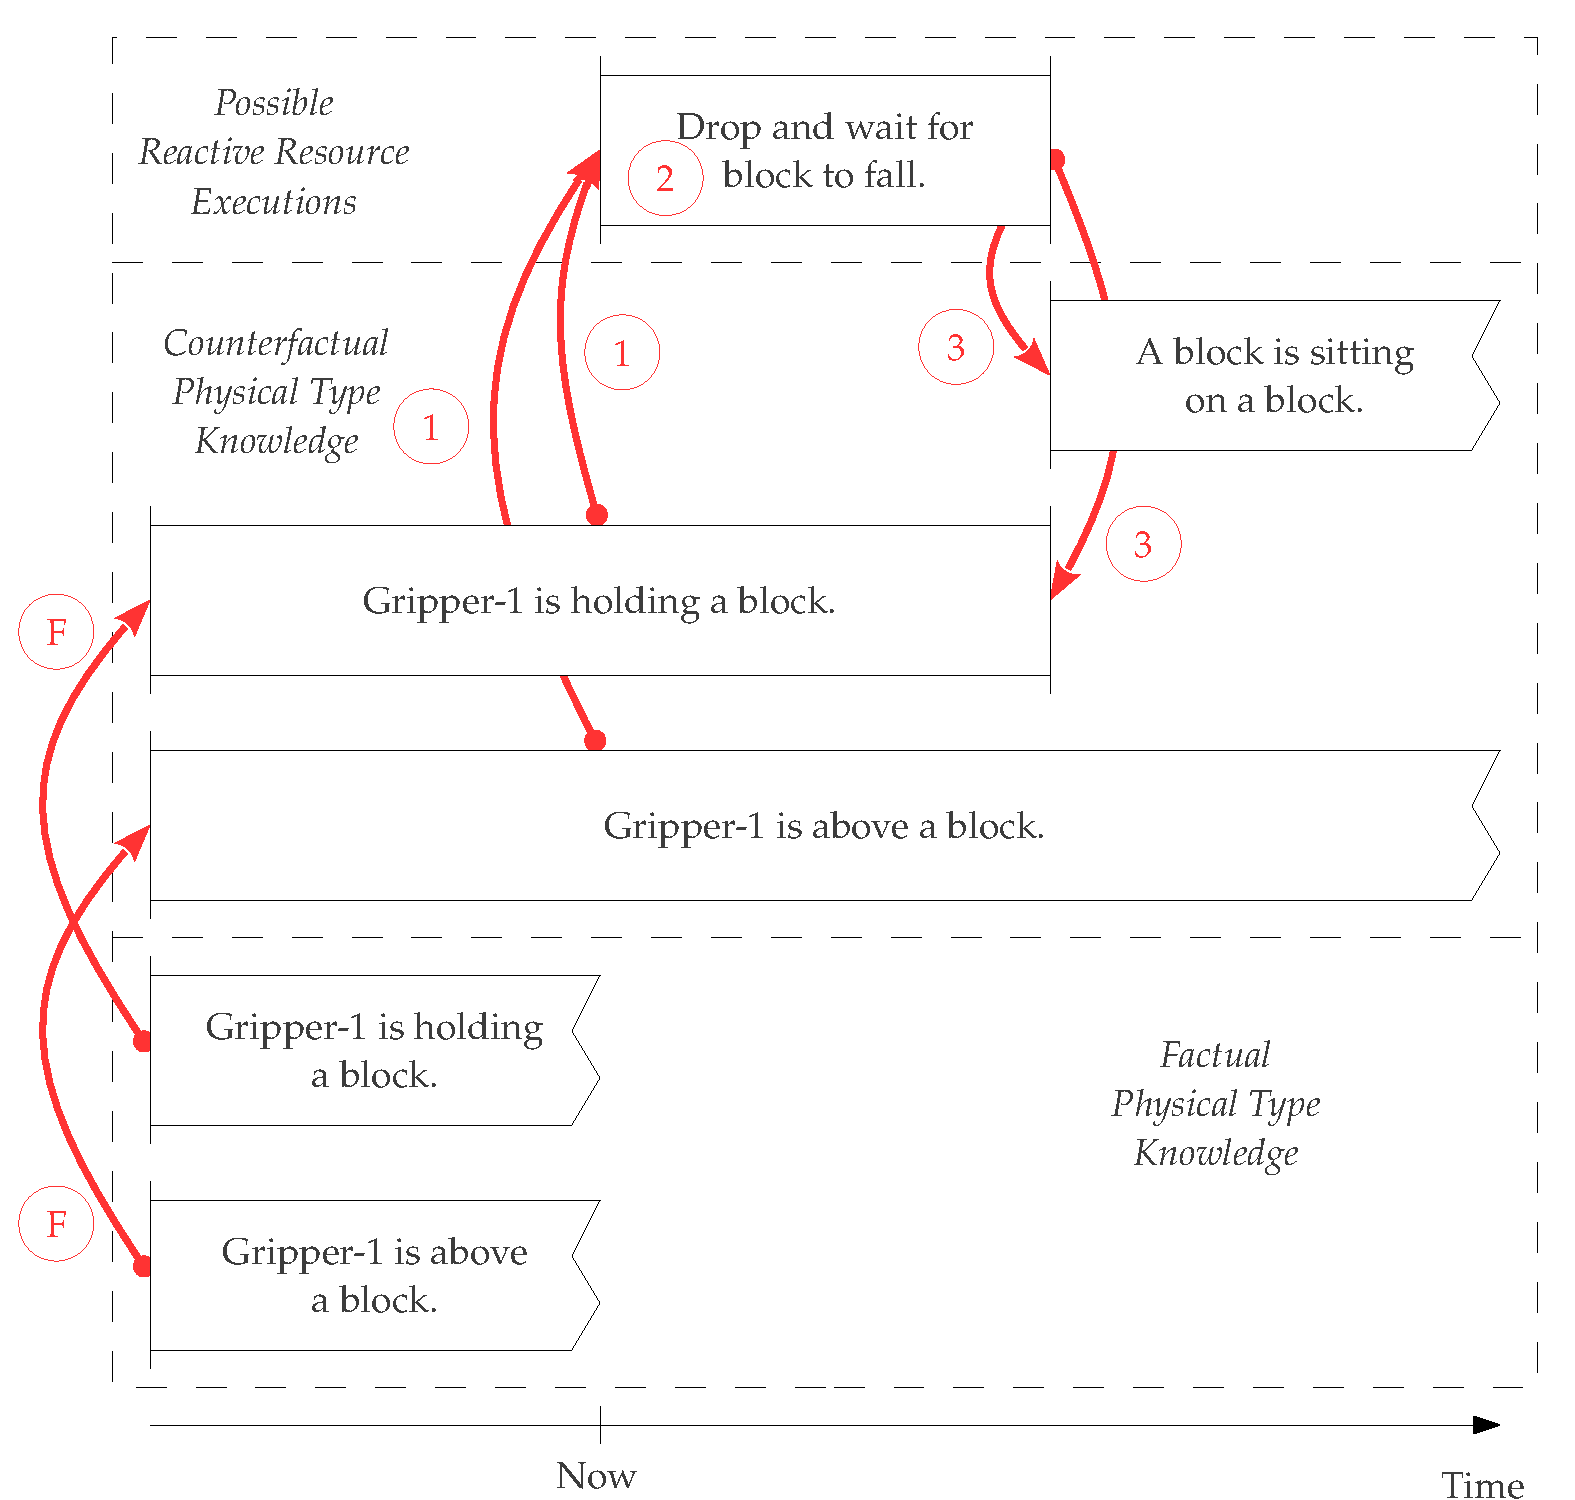
\includegraphics[width=12cm]{gfx/inference_of_physical_knowledge}
%% \caption[Inference of counterfactual physical type knowledge from
%%   factual physical type knowledge.]{Inference of counterfactual
%%   physical type knowledge from factual physical type knowledge.
%%   Rectangular boxes represent events over time.  Some events have a
%%   jagged right edge to indicate that this event has no ending time.
%%   Curved arrows represent different dependency relationships: (F)
%%   factual, (1) precondition, (2) potential resource execution, and (3)
%%   hypothetical change.  Preconditions, potential resource executions,
%%   and hypothetical changes form the three possibly unsupported parts
%%   of a dependency.  Factual dependencies cannot lose support because
%%   they are derived directly from factual events.}
%% \label{figure:inference_of_physical_knowledge}
%% \end{figure}
%% {\mbox{\autoref{figure:inference_of_deliberative_planning_machine_knowledge}}}
%% shows how the three different types of dependencies analogously relate
%% factual deliberative planning machine type knowledge to counterfactual
%% deliberative planning machine type knowledge through potential
%% deliberative planning resource executions in order to predict
%% hypothetical plan failure in the future.
%% \begin{figure}[h]
%% \centering
%% 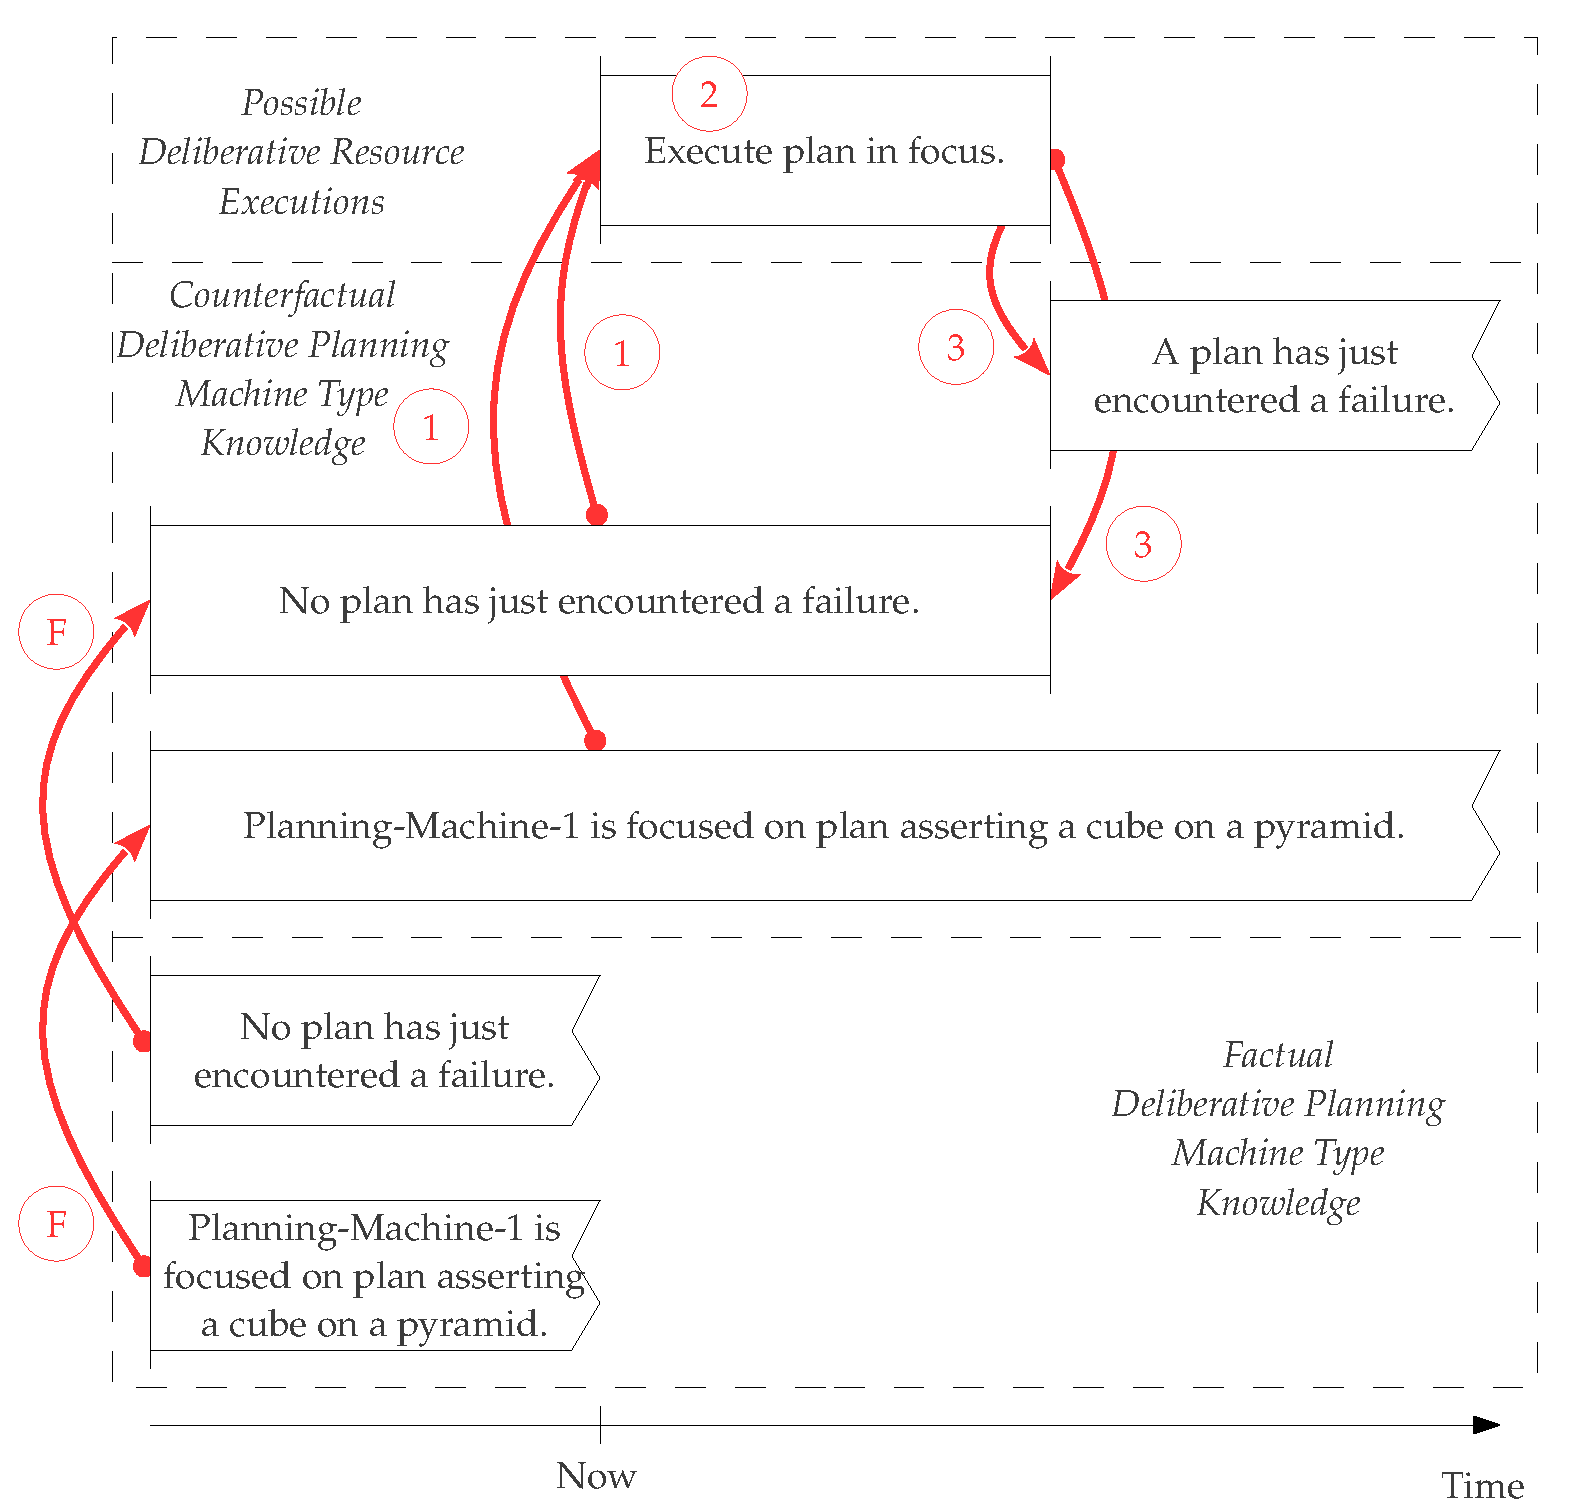
\includegraphics[width=12cm]{gfx/inference_of_deliberative_planning_machine_knowledge}
%% \caption[Inference of counterfactual deliberative planning machine
%%   type knowledge from factual deliberative planning machine type
%%   knowledge.]{Inference of counterfactual deliberative planning
%%   machine type knowledge from factual deliberative planning machine
%%   type knowledge.  Rectangular boxes represent events over time.  Some
%%   events have a jagged right edge to indicate that this event has no
%%   ending time.  Curved arrows represent different dependency
%%   relationships: (F) factual, (1) precondition, (2) potential resource
%%   execution, and (3) hypothetical change.  Preconditions, potential
%%   resource executions, and hypothetical changes form the three
%%   possibly unsupported parts of a dependency.  Factual dependencies
%%   cannot lose support because they are derived directly from factual
%%   events.}
%% \label{figure:inference_of_deliberative_planning_machine_knowledge}
%% \end{figure}


%% \section{Propagating Loss of Hypotheses to Counterfactual Inferences}

%% Plan knowledge that the AI has been told can inform its hypothesis
%% spaces for the potential changes that resource executions will cause,
%% allowing the AI to imagine both successful and unsuccessful
%% accomplishment of the goal condition of ``A block is sitting on a
%% block'' with different hypothetical supports.  When the AI executes
%% the resource, it refines these hypothesis spaces that predict these
%% changes given the factual preconditions and effects of the actual
%% resource execution.  The refinement of hypothesis spaces has the
%% potential to eliminate the hypotheses that have supported previous
%% counterfactual inferences.  In order to correct counterfactual
%% inferences when hypotheses are removed from hypothesis spaces, every
%% individual hypothesis in each resource execution transframe change
%% hypothesis space has a list of \emph{removal callbacks} that are
%% called if the hypothesis is ever removed from the hypothesis space.
%% So, when the hypothesis space is refined in light of new factual
%% evidence, dependencies that are supported by these hypotheses are
%% notified that they have become \emph{invalidated}.  When a dependency
%% has become invalidated, it has a chance to reconfigure its
%% hypothetical support, so that it can still predict the same
%% hypothetical change, and thus, still support the counterfactual
%% knowledge that depends upon it.  Here are the basic steps of the
%% grounded hypothesis refinement process that corrects and removes
%% unsupported counterfactual knowledge in light of new evidence and
%% refined hypothesis spaces:
%% \begin{enumerate}
%% \item When a resource execution transframe change hypothesis space is
%%   refined, removing hypotheses, registered callbacks for each of these
%%   hypotheses are called, invalidating the dependencies that are
%%   supported by these hypotheses.
%% \item Invalidated dependencies check to see if the resource execution
%%   transframe change hypothesis space still contains hypotheses that
%%   will support the change given the preconditions for the possible
%%   resource execution.
%% \item If the invalidated dependency can find new hypothetical support
%%   for the resource execution transframe change, it marks itself as
%%   valid and no counterfactual events are modified as the dependency
%%   has found new supporting hypotheses.
%% \item If the invalidated dependency cannot find new hypothetical
%%   support for the resource execution transframe change, it becomes
%%   unsupported and marks dependent counterfactual knowledge to be
%%   unsupported and removed from the counterfactual knowledge base.
%% \item If a counterfactual event loses the support of a dependency and
%%   is removed from the counterfactual knowledge base, those
%%   dependencies that are supported by these counterfactual events as
%%   preconditions are invalidated, causing the propagation of the
%%   refined hypothesis spaces to correct further counterfactual event knowledge.
%% \end{enumerate}

%% In this way, as hypothesis spaces are refined and hypotheses are
%% eliminated due to new factual evidence, the effects on the
%% counterfactual knowledge is minimized by first invalidating the
%% dependencies, allowing them to rearrange their supports where
%% possible, before dependencies give up and declare themselves as
%% unsupported to their dependent counterfactual events.

%% \section{Losing and Searching for New Hypothetical Support}

%% When the AI first imagines that executing its plan will result in ``A
%% cube is sitting on a pyramid,'' this counterfactual event is
%% associated with the newly created dependency shown in
%% {\mbox{\autoref{table:physical_dependency}}}.
%% \begin{table}[h]
%% \centering
%% \begin{tabular}{c}
%%   A Supported Dependency for Counterfactual \\
%%   Physical Type Knowledge Event \\
%%   ``A cube is sitting on a pyramid.'' \\
%%   \begin{tabular}{|p{3cm}|p{6cm}|}
%%     \hline
%%     \emph{possible resource execution:} & Drop and wait for block to fall. \\
%%     \hline
%%     \emph{preconditions:}               & \\
%%     \hline
%%     \emph{add hypotheses:}              & \emph{True} \\
%%     \hline
%%   \end{tabular}
%% \end{tabular}
%% \caption[A dependency for a counterfactual physical type knowledge
%%   event given no factual evidence.]{A dependency for a counterfactual
%%   physical type knowledge event given no factual evidence.  Notice
%%   that since this knowledge has ``been told'' to the AI without any
%%   experience executing this action, the hypothesis space has not been
%%   refined and the most general hypothesis, which predicts \emph{True}
%%   in all preconditions, is the only supporting hypothesis for this
%%   counterfactual event.}
%% \label{table:physical_dependency}
%% \end{table}
%% When the AI actually executes the ``Drop and wait for block to fall
%% resource'', the hypothesis space for the addition of ``A cube is
%% sitting on a pyramid'' is refined by removing those hypotheses that
%% are no longer consistent with the factual event knowledge.  The
%% hypothesis space reflects that in the specific preconditions of the
%% execution, the change did not occur.  However, the AI is not sure
%% about other possible preconditions.  In this case, the most general
%% hypothesis, which is \emph{True} in all preconditions, has been
%% removed from the hypothesis space.  This causes the dependency shown
%% in {\mbox{\autoref{table:physical_dependency}}} to become invalidated.
%% The dependency then attempts to find new hypothetical support for its
%% predicted change.  In this case, the dependency is not able to
%% reconfigure its support in order to mark itself as once again valid,
%% so the dependency becomes unsupported and removes the unsupported
%% counterfactual event that depends upon it.  The unsupported dependency
%% due to the loss of the most general hypothetical support is shown in
%% {\mbox{\autoref{table:physical_reconfigured_dependency}}}.
%% \begin{table}[h]
%% \centering
%% \begin{tabular}{c}
%%   An Unsupported Dependency for Counterfactual \\
%%   Physical Type Knowledge Event \\
%%   ``A cube is sitting on a pyramid.'' \\
%%   \begin{tabular}{|p{3cm}|p{6cm}|}
%%     \hline
%%     \emph{possible resource execution:} & Drop and wait for block to fall. \\
%%     \hline
%%     \emph{preconditions:}               & $A$: Gripper-1 is holding a block. \\
%%                                         & $B$: Gripper-1 is above a cube. \\
%%     \hline
%%     \emph{add hypotheses:}              & ${\neg}A \wedge B$ \\
%%                                         & $A \wedge {\neg}B$ \\
%%                                         & ${\neg}A \wedge {\neg}B$ \\
%%     \hline
%%   \end{tabular}
%% \end{tabular}
%% \caption[An unsupported dependency for a counterfactual physical type
%%   knowledge event after losing its original hypothetical support and
%%   attempting to reconfigure new support.]{An unsupported dependency
%%   for a counterfactual event after losing its original hypothetical
%%   support due to experience executing the reactive resource.  Note
%%   that this dependency has found a number of hypotheses that would
%%   provide support under different preconditions.}
%% \label{table:physical_reconfigured_dependency}
%% \end{table}

%% Initially the reflective layer of the AI has not been told any plans
%% that assert conditions of the deliberative planning machine type
%% knowledge.  This means that when the reflective layer imagines
%% executing the plan in focus, it does not predict a failure will occur.
%% However, when the AI has executed the plan to stack the cube on the
%% pyramid, this actually does result in a factual failure.  The AI
%% reflectively responds to the failure by imagining executing a new plan
%% for deliberative action.  The reflective layer infers the
%% counterfactual deliberative planning machine type knowledge shown in
%% {\mbox{\autoref{figure:inference_of_deliberative_planning_machine_knowledge}}}.
%% During this imaginative inference process, the reflective layer
%% creates the counterfactual event, ``A plan has just encountered a
%% failure'', which has the newly created dependency shown in
%% {\mbox{\autoref{table:deliberative_dependency}}}.
%% \begin{table}[h]
%% \centering
%% \begin{tabular}{c}
%%   A Supported Dependency for Counterfactual \\
%%   Deliberative Planning Machine Type Knowledge Event \\
%%   ``A plan has just encountered a failure.'' \\
%%   \begin{tabular}{|p{3cm}|p{6cm}|}
%%     \hline
%%     \emph{possible resource execution:} & Execute plan in focus. \\
%%     \hline
%%     \emph{preconditions:}               & $A$: No plan has just encountered a failure. \\
%%                                         & $B$: Planning-Machine-1 is focused on plan asserting a cube on a pyramid. \\
%%     \hline
%%     \emph{add hypotheses:}              & $A \wedge B$ \\
%%     \hline
%%   \end{tabular}
%% \end{tabular}
%% \caption[A dependency for a counterfactual deliberative planning
%%   machine type knowledge event given no factual evidence.]{A
%%   dependency for a counterfactual deliberative planning machine type
%%   knowledge event given the factual evidence of previously executing
%%   this deliberative resource once in the given deliberative planning
%%   machine type knowledge preconditions.}
%% \label{table:deliberative_dependency}
%% \end{table}
%% With the AI's new experience, it imagines executing another plan,
%% which asserts ``A pyramid is sitting on a cube.''  The execution of
%% the first plan is avoided due to the prediction of failure in the
%% reflective imaginative inference of counterfactual failure for this
%% plan.  When the new plan is selected, it finally succeeds in
%% accomplishing the physical goal condition: ``A block is sitting on a
%% block,'' demonstrating the abstract reflective imagination of plan
%% execution, in this case, helps to accomplish the primary physical goal
%% at hand.

